\documentclass[11pt,a4paper,english]{article}

%%%% PACKAGES WITH OPTIONS
\usepackage[english]{babel}
\usepackage[T1]{fontenc}
\usepackage[margin=2.5cm]{geometry}
\usepackage{lmodern}
\usepackage[utf8]{inputenc}
\usepackage[version=4]{mhchem} % Chemistry and isotopes with \ce{} (other option: 'chemformula' \ch{})
\usepackage[numbers]{natbib} % numbers: needed argument, otherwise error
\usepackage[section]{placeins} % Place floats in their own section
\usepackage[onehalfspacing]{setspace} % Space vertically between lines
\usepackage[raggedright,noindentafter]{titlesec} % Change section/title layout
\usepackage[nottoc,notlot,notlof]{tocbibind} % Include bibliography in table of contents

%%%% PACKAGES WITHOUT OPTIONS
\usepackage{adjustbox} % Use \begin{adjustbox}{center} environment for too wide floats
\usepackage{amsmath, amsfonts, amssymb}
\usepackage{booktabs} % Lines in tables (\<top,mid,bottom>rule)
\usepackage{ctable} % Usage: \ctable[options]{column def like c|c|r|l}{\tnote commands for footnotes}{normal table content}, with \tnote[symbol]{text} footnote definitions, and \tmark[symbol] used to reference the footnote in the normal table content
\usepackage{enumitem} % Lists
\usepackage{flafter} % Place floats after their first appearance in text
\usepackage{float} % [H] modifier for floats etc.
\usepackage{graphicx}
\usepackage{hyperref, cleveref} % Creates links (boxes in various colors around words)
%\usepackage{indentfirst} % Always indent the first line of a section
\usepackage{listings} % Typesetting source code
\usepackage{longtable}
\usepackage{multirow} % For multirow cells in tables
\usepackage{pdfpages} % Include other pdf
\usepackage{physics} % Vector calculus etc.
\usepackage{siunitx} % Fancy display of SI units
\usepackage{subcaption} % Enables subfigures
\usepackage{titling}
\usepackage{xcolor} % Anything with color e.g. \fcolorbox{black}{red}{}
\usepackage{xurl} % Loads package 'url' and breaks urls nicely

%%%% PACKAGES SETUP COMMANDS
\hypersetup{colorlinks=true,
    urlcolor=blue,
    citecolor=gray}
\captionsetup{width=.8\columnwidth,
    %format=hang, % 'Figure n' in front of whole caption
    labelsep=endash,
    justification=centerlast,
    labelfont={bf}}
\titleformat{\paragraph}[hang]{\normalfont\normalsize\bfseries}{\theparagraph}{1em}{}
\titlespacing*{\paragraph}{0pt}{3.25ex plus 1ex minus .2ex}{0.5em}

%%%% (RE)NEWCOMMAND
% Bold and italic vector symbols (preferably use \vb{} instead)
\renewcommand{\vec}[1]{\boldsymbol{#1}}
% Mono-spaced inline code (for multiline code, use package 'listings')
\newcommand{\code}[1]{\texttt{#1}}
% Equals sign, with number above referencing some equation
\newcommand{\numeq}[1]{\stackrel{\scriptscriptstyle(\mkern-1.5mu#1\mkern-1.5mu)}{=}}
% If-and-only-if sign, with number above referencing some equation
\newcommand{\numiff}[1]{\stackrel{\scriptscriptstyle(\mkern-1.5mu#1\mkern-1.5mu)}{\Leftrightarrow}}
% Numbers a single line in a no-numbering multiline equation* or align*
\newcommand{\numberthis}{\addtocounter{equation}{1}\tag{\theequation}}
% MuMax3
\newcommand{\mumax}{$\mathsf{mumax}^3$}
% Vertical line between subplots
\newcommand{\rulesep}{\unskip\ \vrule\ }

%%%% EXTRA SYMBOLS
\DeclareSymbolFont{extraitalic}      {U}{zavm}{m}{it}
\DeclareMathSymbol{\Qoppa}{\mathord}{extraitalic}{161}
\DeclareMathSymbol{\qoppa}{\mathord}{extraitalic}{162}
\DeclareMathSymbol{\Sampi}{\mathord}{extraitalic}{165}
\DeclareMathSymbol{\sampi}{\mathord}{extraitalic}{166}
\DeclareMathSymbol{\Stigma}{\mathord}{extraitalic}{167}
\DeclareMathSymbol{\stigma}{\mathord}{extraitalic}{168}

%%%% DOCUMENT
\begin{document}

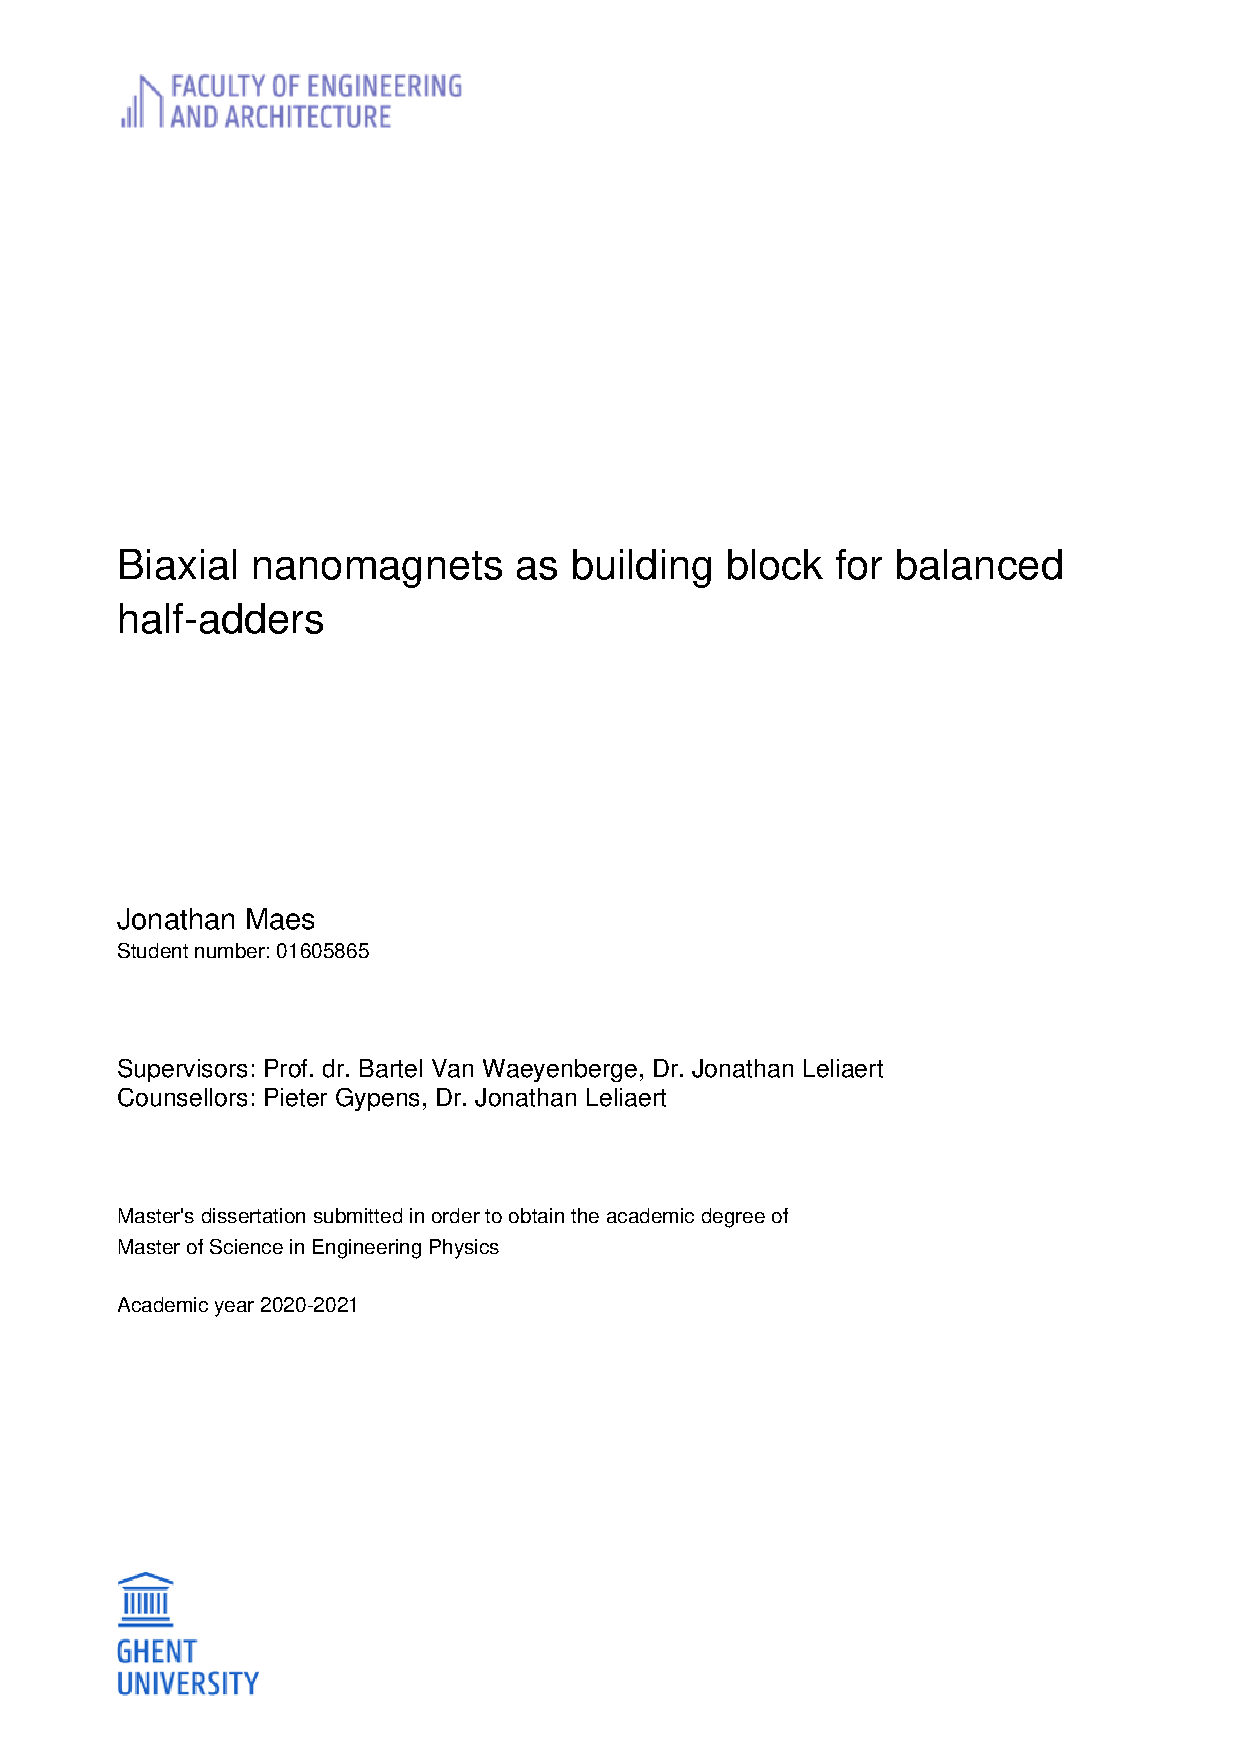
\includepdf[pages={1}]{Frontpage.pdf} % (download from plato.ea.ugent.be)
\shipout\null % Blank page
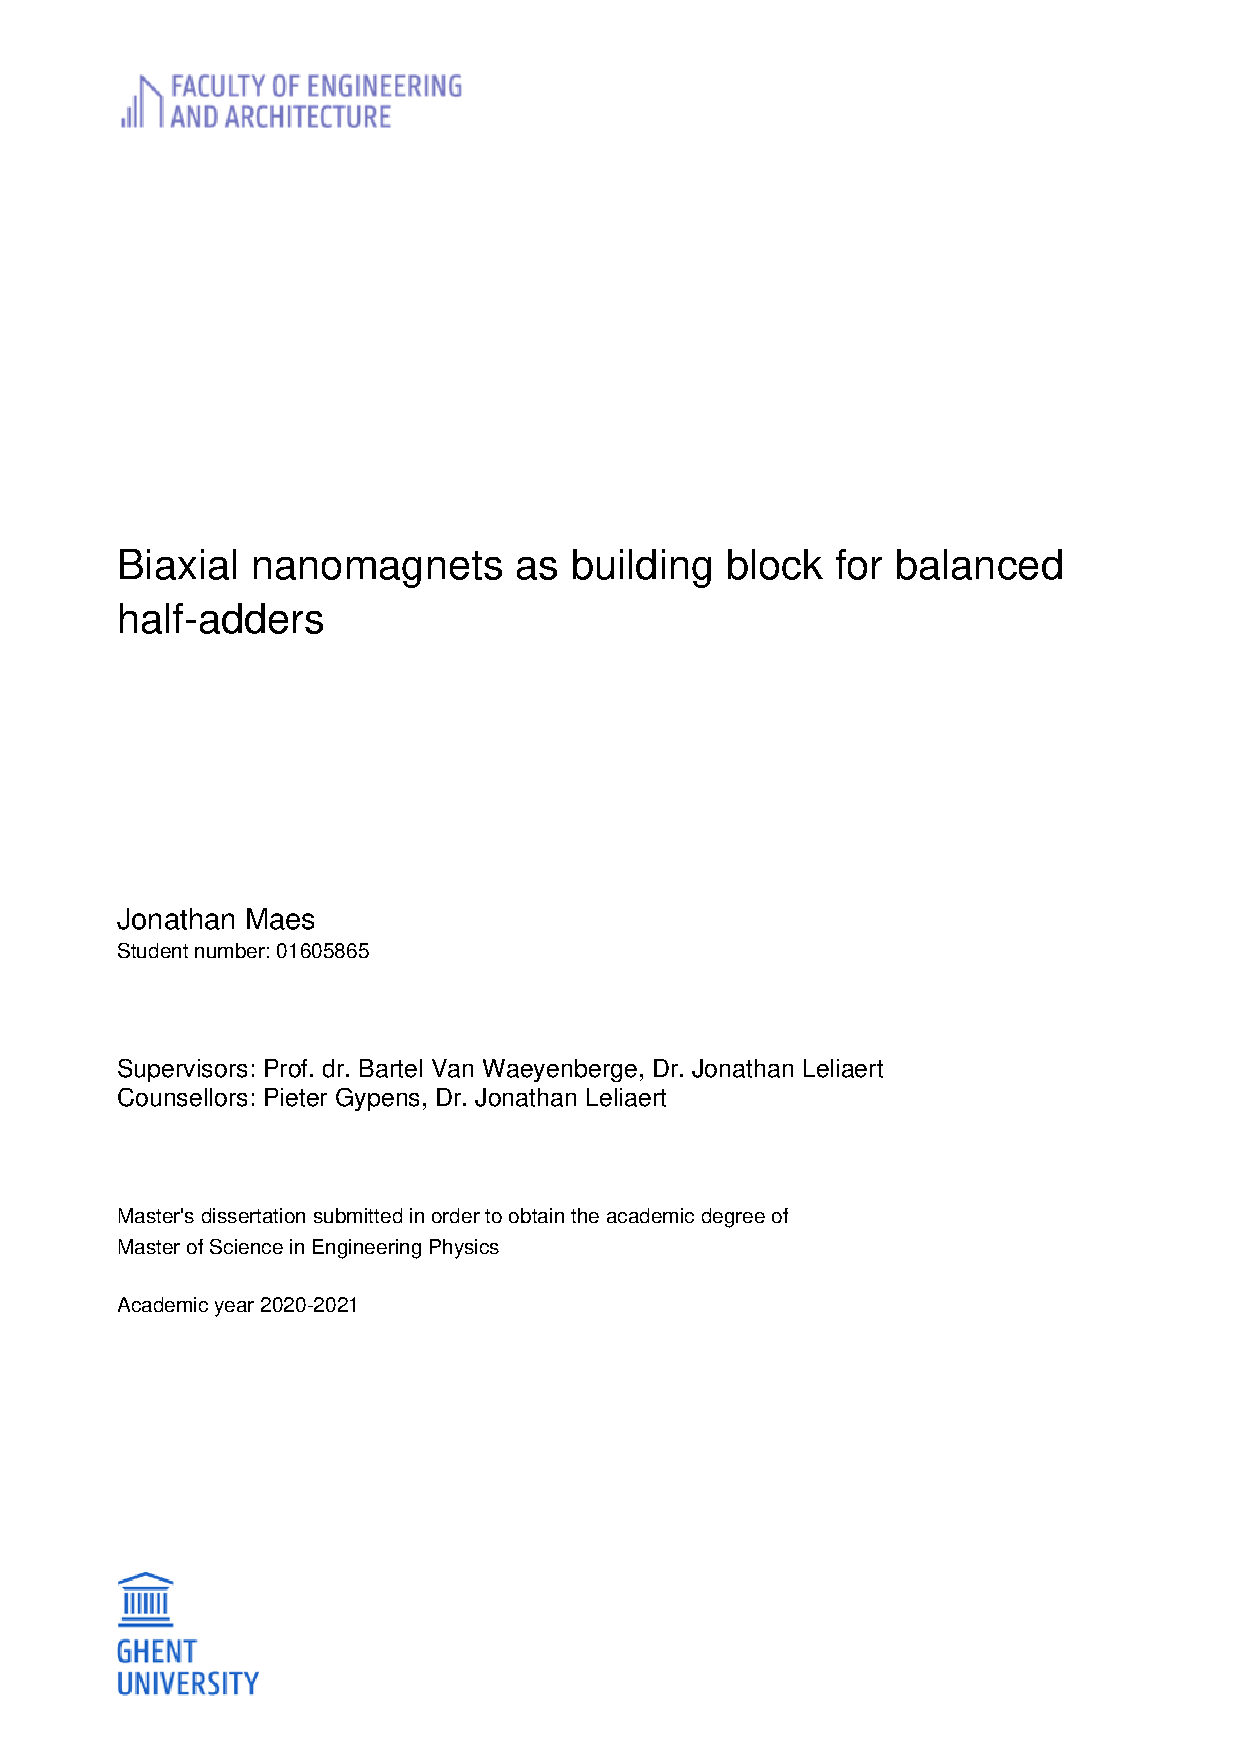
\includepdf[pages={1}]{Frontpage.pdf} % (download from plato.ea.ugent.be)

% TODO op het einde: spellingcheck
% <te gebruiken> ipv <wat er staat>:
% - ization ipv isation
% - centre ipv center
% - island ipv droplet
% - chain ipv wire
% TODO op het einde: bibliografie check
% - Volgorde in tekst zelf: bv. niet [36,34] maar wel [34,36]
% - Kijken of er geen vreemde tekst in de bibliografie staat
\newpage
\pagenumbering{roman}

\begin{center}
    The author(s) gives (give) permission to make this master dissertation available for consultation and to copy parts of this master dissertation for personal use. In all cases of other use, the copyright terms have to be respected, in particular with regard to the obligation to state explicitly the source when quoting results from this master dissertation.
\end{center}
\subsection*{Acknowledgements} % TODO: Acknowledgements
I would like to thank Jonathan Leliaert and Pieter Gypens for their regular suggestions and supervision, which was indispensible to achieving a sufficient understanding of nanomagnetic logic.

\clearpage
\begin{center}
    \Large
    \textbf{Biaxial nanomagnets as building block for balanced half-adders}

    \large
    \vspace{0.4cm}
    Jonathan Maes
       
    \vspace{0.9cm}
    \textbf{Abstract}
\end{center}
Nanomagnetic logic makes use of magnetostatic interactions to implement logic gates. These logic gates are constructed by placing several nanomagnetic islands in close vicinity. Their dipolar interaction then implements the logical functionality. The magnetization direction of a single island can be identified with a bit. Nanomagnetic islands with biaxial anisotropy have four stable directions, such that each island can represent exactly two bits. This should allow for a higher integration density as compared to uniaxial anisotropy. Since every nanomagnet influences every other nanomagnet, and vice versa, there exists a two-way flow of information between the input and output. This allows for reverse calculations, but only if the ground states of all four possible inputs have equal energy. If this is the case, the gate is termed `balanced'.
Now talk about what was noted in this thesis. Like for example the things in the conclusion, but condensed to fit on this one page. % TODO: Abstract + keywords (max. 1 page)
\vspace*{\fill}
{\small Keywords: biaxial, nanomagnetic logic, half adder}

% TODO: Extended abstract (2-6 pages)

\clearpage
{\hypersetup{linkcolor=black}
\tableofcontents
}
\newpage
% TODO: op het einde een symbool vervangen door \sampi voor de lol
\subsection*{List of constants}
\begin{longtable}{llll}
\toprule
\bfseries Symbol & \bfseries Name &
\bfseries Value \\\midrule\endhead
$k_B$ & Boltzmann constant & \SI{1.380649e-23}{\joule\per\kelvin} \\
\midrule
$\gamma$ & Gyromagnetic ratio & \SI{1.7595e11}{\radian\per\tesla\per\second} \\
$\gamma_0$ & $\mu_0 \gamma$ & \SI{2.2111e5}{\metre\per\ampere\per\second} \\
$\mu_0$ & Vacuum permeability & $4\pi\SI{e-7}{\henry\per\metre}$ \\
\bottomrule
\end{longtable}

\subsection*{List of abbreviations}
\begin{longtable}{llll}
\toprule
\bfseries Abbreviation & \bfseries Full name \\\midrule\endhead
AFM & Anti-ferromagnetic \\
BCC & Body-centered cubic \\
CMOS & Complementary metal-oxide-semiconductor \\
EQCA & Electronic quantum cellular automata \\
FCC & Face-centered cubic \\
FD & Finite difference \\
FM & Ferromagnetic \\
FSAL & First-same-as-last \\
GPU & Graphics processing unit \\
LL & Landau-Lifshitz \\
LLG & Landau-Lifshitz-Gilbert \\
MFM & Magnetic force microscopy \\
MOKE & Magneto-optical Kerr effect \\
MQCA & Magnetic quantum cellular automata \\
MTXM & Magnetic transmission X-ray microscopy \\
NML & Nanomagnetic logic \\
PEEM & Photoelectron emission microscopy \\
QCA & Quantum cellular automata \\
XMCD & X-ray magnetic circular dichroism \\
\bottomrule
\end{longtable}

\subsection*{List of symbols}
A bold symbol indicates a vector.
\begin{longtable}{llll}
\toprule
\bfseries Symbol & \bfseries Name &
\bfseries Unit \\\midrule\endhead
$\vb{a}$ & Unit vector & \\
$A_{ex}$ & Exchange stiffness constant & \si{\joule\per\metre} \\
$B_1$ & First balancedness metric: $\min_\alpha(E_{\alpha,1}) - \max_\alpha(E_{\alpha,0})$ & \si{\joule} \\
$B_2$ & Second balancedness metric: $\max_\alpha(E_{\alpha,0}) - \min_\alpha(E_{\alpha,0})$ & \si{\joule} \\
$\vb{B}$ & Magnetic flux density & \si{\tesla} \\
$\vb{B_{ext}}$ & External field flux density & \si{\tesla} \\
$\vb{B_{ext,v}}$ & Virtual external field flux density & \si{\tesla} \\
$d$ & Distance between centers of two islands & \si{\metre} \\
$\vb{e_i}$ & Unit vectors along the axes of cubic anisotropy &  \\
$E$ & Energy & \si{\joule} \\
$E_{\alpha,i}$ & $i$-th energy level for which the input magnetization angle is near $\alpha$ & \si{\joule} \\ 
$E_{anis}$ & Anisotropy energy & \si{\joule} \\
$E_{barrier}$ & Energy barrier between stable states & \si{\joule} \\
$E_{demag}$ & Demagnetization energy & \si{\joule} \\
$E_{exch}$ & Exchange energy & \si{\joule} \\
$E_{me}$ & Magneto-elastic energy & \si{\joule} \\
$E_{Zeeman}$ & Zeeman energy & \si{\joule} \\
$f_0$ & Attempt frequency & \si{\hertz} \\
$\vb{H}$ & Magnetic field strength & \si{\ampere\per\metre} \\
$\vb{H_{demag}}$ & Demagnetizing field & \si{\ampere\per\metre} \\
$\vb{H_{eff}}$ & Effective field & \si{\ampere\per\metre} \\
$\vb{H_{ex}}$ & Exchange field & \si{\ampere\per\metre} \\
$\vb{H_{ext}}$ & External field & \si{\ampere\per\metre} \\
$\vb{H_{therm}}$ & Stochastic thermal field & \si{\ampere\per\metre} \\
$I_{XMCD}$ & Intensity of XMCD signal & \si{\watt\per\metre\squared} \\
$J_{ij}$ & Exchange integral for spins $i$ and $j$ & \si{\joule} \\
$K_{c1}$ & First order cubic anisotropy constant & \si{\joule\per\metre\cubed} \\
$K_{c2}$ & Second order cubic anisotropy constant & \si{\joule\per\metre\cubed} \\
$K_{u1}$ & First order uniaxial anisotropy constant & \si{\joule\per\metre\cubed} \\
$K_{u2}$ & Second order uniaxial anisotropy constant & \si{\joule\per\metre\cubed} \\
$L$ & Ellipse major axis & \si{\metre} \\
$\vb{m}$ & Reduced magnetization $\vb{M}/M_{sat}$ &  \\
$\vb{m_i}$ & Magnetic moment of atom $i$ & \si{\ampere\metre\squared} \\
$\vb{M}$ & Magnetization & \si{\ampere\per\metre} \\
$M_{sat}$ & Saturation magnetization & \si{\ampere\per\metre} \\
$\vb{n_i}$ & Unit vector in the direction of $\vb{S_i}$ &  \\
$N$ & Number of switches during a time interval $\tau$ &  \\
$P_i$ & Uniformly random number between 0 and 1 &  \\
$\vb{r}$ & Position vector & \si{\metre} \\
$\vb{s}$ & Lattice displacement field & \si{\metre} \\
$\vb{S_i}$ & Spin of atom $i$ &  \\
$t$ & Time & \si{\second} \\
$t_i$ & Time between thermal switch $i$ and $i+1$ & \si{\second} \\
$T$ & Temperature & \si{\kelvin} \\
$T_C$ & Curie temperature & \si{\kelvin} \\
$T_N$ & N\'{e}el temperature & \si{\kelvin} \\
$\vb{u}$ & Unit vector along the axis of uniaxial anisotropy &  \\
$V$ & Volume of single-domain particle & \si{\metre\cubed} \\
\midrule
$\alpha$ & Gilbert damping constant &  \\
$\alpha'$ & $\frac{\alpha \gamma_0}{1+\alpha^2}$ &  \\
$\alpha_i$ & Orientation of geometry of island $i$ & \si{\radian} \\
$\gamma_0'$ & $\frac{\gamma_0}{1+\alpha^2}$ & \si{\radian\metre\per\coulomb} \\
$\Delta t$ & Time step of numerical update scheme & \si{\second} \\
$\vec{\eta}$ & Random vector from standard normal distribution &  \\
$\theta$ & Inclination in spherical coordinates & \si{\radian} \\
$\Theta_i$ & Instantaneous magnetization angle in the horizontal plane of island $i$ & \si{\radian} \\
$\widetilde{\Theta}_i$ & Relaxed magnetization angle in the horizontal plane of island $i$ & \si{\radian} \\
$\lambda$ & Exchange length & \si{\metre} \\
$\rho$ & Ellipse roundness: ratio between major and minor axes &  \\
$\sigma$ & Photon spin & \si{} \\
$\tau$ & Total simulation time & \si{\second} \\
$\phi$ & Azimuth in spherical coordinates & \si{\radian} \\
$\Phi_i$ & Rotation of island $i$ geometry & \si{\radian} \\
$\chi$ & Angle of real external field in the horizontal plane & \si{\radian} \\
$\widetilde{\chi}_i$ & Angle of virtual external field in the horizontal plane for island $i$ & \si{\radian} \\
$\psi$ & Vector potential & \\
$\Omega_i$ & Geometry of ferromagnetic region $i$ in the finite-difference grid & \\
\bottomrule
\end{longtable}



\cleardoublepage
\pagenumbering{arabic}
\section{Introduction}
%\noindent \textit{Note: This section exists to explain nanomagnetic logic to the unfamiliar reader. \textbf{Biaxial island} begins the investigation of the dynamics of a single biaxial island, and is a suitable starting point for those already familiar with nanomagnetic logic.} \bigskip

\noindent The goal of this thesis is to design a nanomagnetic logic gate that can function as a half adder. This gate will be built from biaxial nanomagnets, whose dipolar interaction will ensure that the gate self-organizes into the logically correct states. Ideally, this gate should also be balanced, meaning that all its ground state energies are equal, such that a reverse calculation is possible. Let us first break down the different concepts underlying nanomagnetic logic from the ground up. \par % TODO: this ultra-first paragraph a bit more clear
An atom may display what is called a \textbf{magnetic dipole moment}, on one hand due to the angular momentum of electrons around the nucleus, and on the other hand due to the intrinsic spin of the elementary particles which make up the atom. The magnetic moment can be defined using the torque the atom experiences in a magnetic field.~\cite{IntroMagneticMaterials} In a material, many atoms are together, and the macroscopic sum of all their magnetic moments is called the magnetization of the material. In a crystalline material, the periodicity of the lattice can give rise to specific orderings of the magnetic moments, like for example ferromagnetism where all individual magnetic moments of neighboring atoms try to align themselves in the same direction. \par 
Such a ferromagnetic material, like iron, nickel or cobalt, consists of many \textbf{magnetic domains}. Each domain, on the order of several tens of micrometers, has a nearly uniform magnetization pointing in a random direction. Because the direction of each domain is random, a ferromagnetic material does not display a macroscopic net magnetization. However, when one fabricates a very small island of several hundred nanometers made of such a ferromagnetic material, it will not be made up of several domains, but rather only one, and will thus have a nearly uniform magnetization. \par
If this island has one or another form of anisotropy, be it due to the crystal structure or the shape of the island, the magnetization will have minimal energy if it lies along a certain axis, called the `easy axis'. \textbf{Shape anisotropy} originates from the observation that the magnetization of a domain preferably orients itself along the long axis of a microscopic structure. An example that is often used is a 2D ellipse, for which the easy axis is equal to the long axis of the ellipse. In general, if a structure has one easy axis (and thus two stable directions), we speak of uniaxial anisotropy. In the case of two easy axes (and thus four stable directions), as will be the main topic of this thesis, this is called biaxial anisotropy. Biaxial shape anisotropy can be achieved with a geometry that is invariant under rotation over \SI{90}{\degree}. \par
In the uniaxial case, there are two stable directions, which can be related to a `0' or `1' bit. Hence, these nanomagnetic islands can be used to create a \textbf{digital logic circuit}. Nanomagnetic logic (NML) computing architectures propagate binary information by relying on dipolar field coupling to reorient closely spaced nanoscale magnets.~\cite{SubnanosecondPropagation_AnisotropyChains} This architecture is promising for its extremely low energy dissipation per operation.~\cite{SubnanosecondPropagation_AnisotropyChains,FourStateLogic,MQCA_RoomTemp} One can use nanomagnetic logic to perform normal logic operations, which propagate information from an input to an output. However, this does not give NML an edge over CMOS-based technologies, as one still needs clocking to perform such logic operations. \par 
A fundamentally different way of thinking about logic, which can give NML an edge over CMOS, is provided by `terminal-agnostic' logic.~\cite{FactorizationMemcomputing} A terminal-agnostic gate should be able to self-organize into its logically correct states, such that it does not matter whether the information is fed at what would traditionally be considered the input or output. A way of achieving this using NML, is by making use of `\textbf{balanced}' gates. These are gates for which the ground states corresponding to all possible inputs have the same energy.~\cite{GYP-18} As such, at nonzero temperatures there is an equal chance that the gate is in any of the correct logical states, irrespective of whether the information was fed at the traditional input or output.~\cite{gypens2020nanomagnetic} As such, one can perform reversible logic operations, as by applying the desired output one can recover the corresponding input. \par % TODO: maybe look at this explanation one more time
There have been examples in literature where majority logic gates and balanced NAND gates have been created using nanomagnets.~\cite{GYP-18} Biaxial nanomagnets can be used to encode two bits in one island, because those have 4 stable magnetization directions. This should allow for smaller logic gates due to the increased integration density as compared to uniaxial islands. The main goal of this thesis is to realize a half adder using biaxial nanomagnets. A half adder takes two bits as input and yields two bits as output, so it feels almost natural to design it using biaxial nanomagnets instead of uniaxial ones.


In the following sections, the nature of magnetism and magnetic domains, the concept of quantum cellular automata, signal propagation and techniques for imaging the magnetization will be explained in more detail.

\subsection{Domains}
In 1907, Weiss proposed the idea that a ferromagnetic material contains several uniformly magnetized domains, but that the magnetization of each domain individually is random, thus resulting in a macroscopic zero net magnetization of a large amount of material.~\cite{MuMax3_advances} These domains should not be confused with grains, which are only related to the crystallography. The uniform alignment inside a single domain is due to the quantum mechanical Heisenberg-Dirac exchange interaction.~\cite{MuMax3_advances, heisenberg1928theorie} The magnetostatic energy makes it unfavorable for neighboring moments to align themselves parallel to one another, which competes with the exchange energy which tends to align neighboring moments in the same direction. Since the exchange energy only acts on small length scales, domains are formed under the influence of the exchange energy, while different domains tend to cancel out each other's fields due to the magnetostatic energy. \par
The typical size of these domains is on the order of several tens of micrometers. When the size of the material becomes on the order of micrometers, the domains form very symmetric patterns in order to minimize their energy, and on even smaller length scales only one single domain remains.~\cite{NML_Carlton} So, if one makes a droplet of ferromagnetic material smaller than this typical size, the droplet will have a nearly uniform magnetization, with a magnitude equal to the saturation magnetization of the material.~\cite{NML_Carlton} Such a small droplet can for example be produced using electron beam lithography.~\cite{MQCA_RoomTemp, NML_Carlton} \par
By introducing anisotropy in the droplet, one or more axes can be made energetically favorable for the magnetization. This anisotropy can have two origins: magnetocrystalline anisotropy favors the crystallographic axes, while shape anisotropy can be realized by giving the droplet an elongated shape, for example an ellipse instead of a perfect circle. In the uniaxial case, there is one stable magnetization axis, so the two directions `up' and `down' along this axis can be related to bits `0' and `1'.~\cite{MQCA_RoomTemp} This is not to be confused with unidirectional anisotropy, which only has one stable magnetization direction, and can be achieved using the exchange bias effect.~\cite{ExchangeBias_Mechanisms,ExchangeBias_nanostructures,ExchangeBias} A lot of research has been conducted to use uniaxial anisotropy for computation, and logic gates and wires have been proposed, which use classical magnetostatic interactions to propagate the information.~\cite{GYP-18,MQCA_MajorityGate,SwitchingForced_EnergyEfficient} The use of two favorable axes, i.e. biaxial anisotropy, allows for a higher logic density, as the four stable directions `up', `down', `right' and `left' can be related to `00', `01', `10' and `11'.~\cite{MQCA_ImageRecognition} This can occur for cubic crystals, and can also be realized by giving the shape of the droplet more symmetry, for example by making the shape the union of two ellipses.


\subsection{Quantum Cellular Automata}
Traditional digital logic technologies like CMOS use field-effect transistors to control the flow of electrons. This kind of architecture fundamentally only allows information to flow in one direction. Other architectures allowing communication between the output and input in both ways could allow certain types of computations to be executed faster. One approach to realizing such an architecture are the Quantum Cellular Automata (QCA), which use quantum effects, in a broad sense, to make logic gates. A cellular automaton is a mathematical concept, proposed by Von Neumann~\cite{Sideinfo_SelfRepAutomata}, in which the universe is divided into a regular grid of cells, where each cell is influenced by its direct neighbors. The most famous example of such a mathematical cellular automaton is Conway's Game of life, which has been shown to be universal for computation, as any Turing machine can be encoded in it.~\cite{QCA_GameOfLife} Apart from the universality in the Turing sense, cellular automata provide an additional benefit because they are able to process algorithms in a distributed manner due to the spatial parallelism inherent to them.~\cite{QCA_GameOfLife} From a practical point of view, QCA can be orders of magnitude smaller and more energy efficient than traditional CMOS technology.~\cite{MQCA_RoomTemp} \par
There are several possibilities to realize QCA, which can generally be classified as either electronic or magnetic QCA. Electronic QCA (EQCA) make use of the forces between electrons, while magnetic QCA (MQCA) leverage the magnetic moments of atoms. EQCA are ``quantum'' because they use quantum mechanical tunneling of charge between quantum dots, while MQCA are ``quantum'' because of the exchange interaction between individual atomic magnetic moments.~\cite{MQCA_RoomTemp} Apart from this quantum mechanical nature of the building blocks, QCA are essentially classical devices switching through either coulombic or magnetic interactions.~\cite{QCA_Algorithms} What all these QCA have in common, is that every fundamental building block (electrons, magnetic moments...) of these automata influences every other building block in the automaton, thus allowing the aforementioned two-way flow of information between what would traditionally be referred to as input and output. The MQCA are the main subject of this paper, but it is interesting to take a short look at EQCA as well, for both share some ideas and problems. \par
% Small segue to quantum dot cellular automata
One specific implementation of EQCA makes use of square cells, each with four quantum dots at the vertices of a square. These quantum dots can accomodate an electron, and each cell is made such that there are always two excess electrons present. It is then energetically favorable for these electrons to occupy two diagonally opposite quantum dots.~\cite{QCA_DigitalLogicGate} The two possible diagonal configurations are then the `0' and `1' states. An extensively studied logic gate using this architecture is the three-input majority logic gate. It consists of five cells arranged in a plus-shape, with three inputs and one output. Just like the familiar NAND gate, the majority gate is universal for computation.~\cite{NML_Carlton} By fixing one of the inputs to 0 or 1, an AND or an OR operation can be realized, respectively. A drawback of these EQCA is that they require low electron temperatures in order to work reliably, as otherwise thermal smearing of the charge states of the dots becomes an issue.~\cite{QCA_DigitalLogicGate} \par
QCA compute by relaxing to a configuration of minimal energy.~\cite{QCA_Algorithms} It is important that all these relaxed configurations are equal in energy level. This is what is meant by `balanced' QCA. A necessary condition for an automaton to be balanced is that the number of distinguished configurations with minimum energy should be equal to the number of input combinations the automaton handles.~\cite{QCA_Algorithms}



\subsection{Nanomagnetic islands}
\label{par:Intro_nanomagnetic-islands}
As was mentioned before, the magnetization of a nanomagnetic island tends to align itself along the longest axis of a given geometry. This can be understood as follows. Consider a theoretically ideal island so small that it only consists of two atoms, and thus only two magnetic moments. Four different situations are then shown in~\cref{fig:Intro_IslandEllipticPreferredDirection}.
The first configuration has both magnetic moments vertical and in the same direction, making their magnetic fields line up nicely, forming is a low energy state. In the second configuration, the magnetic moments have opposite direction, such that their fields oppose each other, forming an unfavorable high energy configuration. The third configuration has both moments horizontal in opposite directions, which once again has the magnetic fields nicely lined up in a low energy state. Finally, in the fourth configuration they are pointed horizontal and in the same direction, so the fields once again oppose each other and we have a high energy state. Thus, only two of these four configurations are energetically favorable. \par
Now note that we are only dealing with ferromagnetic materials, which have the property that neighboring moments point in approximately the same direction, due to the exchange energy (\cref{par:Energy_Exchange}). This only leaves the first situation as a stable one, hence explaining the tendency for ferromagnetic materials to be magnetized along the \textbf{long axis of a microscopic geometry}. In larger geometries, however, the third situation is a perfectly acceptable configuration for two separate domains instead of two elementary magnetic moments, but in this thesis we only consider small single-domain islands. In case of higher symmetry, for example with biaxial shape anisotropy, it is no longer clear which symmetry axes will be the easy axes, and which the hard ones, as will be examined in more detail in \cref{par:Biaxial_island}. \par
\begin{figure}[t]
    \centering
    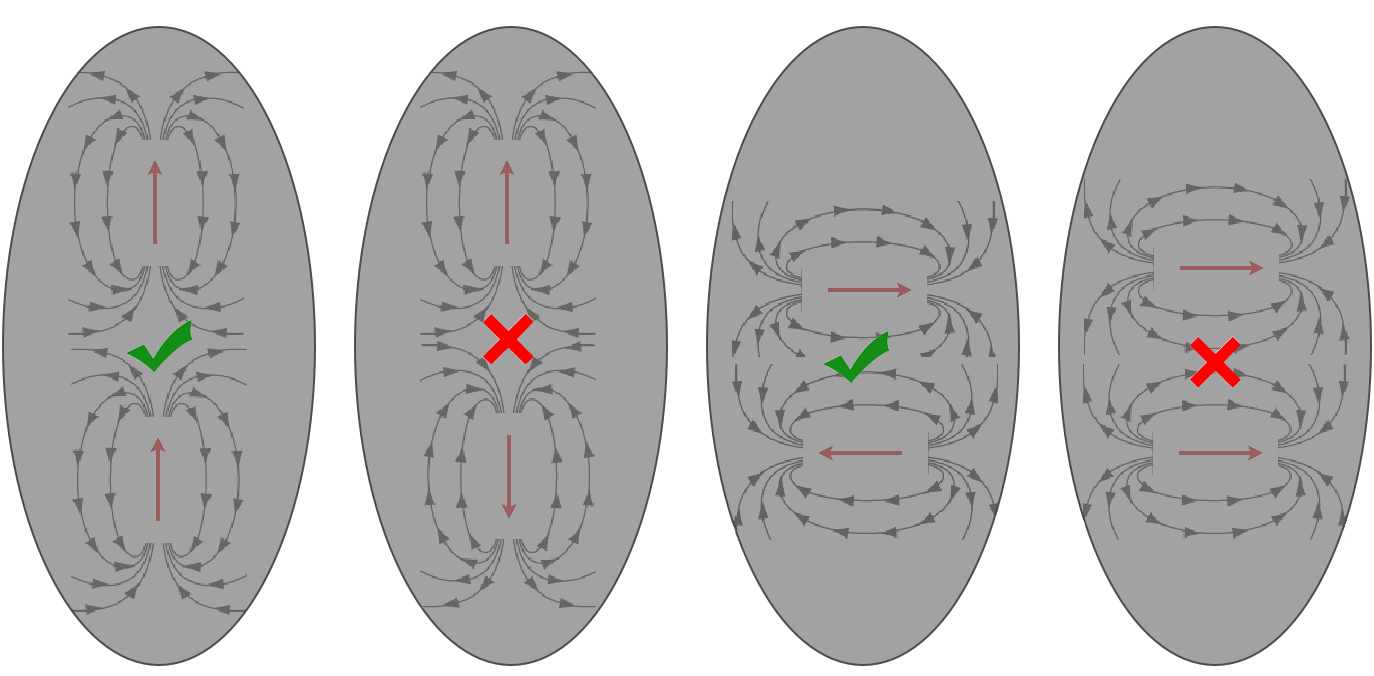
\includegraphics[width=0.8\columnwidth]{Figures/Introduction/NML_Carlton - Figure 1.9 adapted.png}
    \caption{Theoretical situation where an island is made up of two magnetic moments, for four different configurations, explaining the tendency for ferromagnetic materials to be magnetized along the long axis of a microscopic geometric structure. Figure adapted from fig. 1.9 in \cite{NML_Carlton}.}
    \label{fig:Intro_IslandEllipticPreferredDirection}
\end{figure}
When constructing a logic gate, it can be useful to include islands whose magnetization direction is permanently fixed, as opposed to the freely switching islands discussed before. One way to realize such a fixed island is through a phenomenon called `exchange bias'.~\cite{ExchangeBias_Mechanisms,ExchangeBias_nanostructures,ExchangeBias,syllabus_PoAEaPD} This phenomenon arises at the interface between an anti-ferromagnetic (AFM) and a ferromagnetic (FM) material as illustrated in \cref{fig:Intro_ExchangeBias}.
\begin{figure}[t]
    \centering
    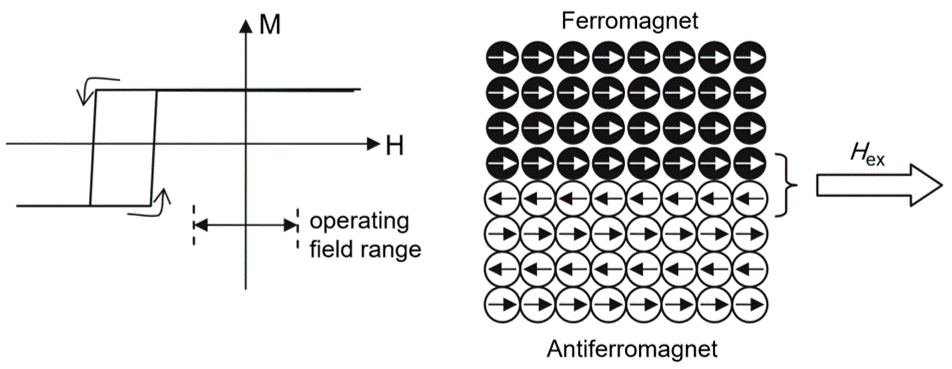
\includegraphics[width=0.8\columnwidth]{Figures/Introduction/Syallabus_PoAEaPD - Figure 2.7.png}
    \caption{The exchange bias effect in ferromagnet/antiferromagnet bilayers with exchange field on the ferromagnetic layer, $\vb{H_{ex}}$, originating from the interface. Figure taken from \cite{syllabus_PoAEaPD}.}
    \label{fig:Intro_ExchangeBias}
\end{figure}
An AFM material consists of magnetic moments which alternate direction in each atomic plane, while in a FM material all these moments point in the same direction. In the situation as illustrated in the figure, the top layer of the AFM material thus also wants the bottom layer of the FM to align anti-parallel, while the FM layer on the contrary prefers a parallel alignment. One of these two competing effects will be stronger than the other, which oftentimes results in an anti-parallel alignment of the magnetic moments at the FM/AFM interface. The AFM material is not affected by external fields, since it consists of alternating magnetic moments leading to a zero net magnetization. The AFM layer will thus remain fixed at temperatures below its N\'{e}el temperature $T_N$. One can define the fixation direction by choosing the materials such that this $T_N$ is lower than the Curie temperature $T_C$ of the FM layer, and first operating at a temperature $T$ for which $T_N < T < T_C$. In this regime, the FM layer will follow an applied magnetic field, while the AFM layer is paramagnetic due to the high temperature. When the temperature is then lowered below $T_N$, the AFM material will settle in such a way that its top layer is correctly aligned as to fix the FM layer.~\cite{ExchangeBias_Mechanisms} \par
At strong enough fields, however, the FM layer will follow the external field anyway, though this will occur at significantly higher fields than for the case where there would be no AFM material. Thus, by manufacturing a FM island on top of an AFM material, the island can be made to have a single preferential direction, instead of a preferential axis. \par
In general, it will be required to fix different islands in different directions. This can not be achieved by heating the whole substrate and applying an external field, so one has to use a local heating process, for example a focused laser beam. By separately heating each island above $T_N$ and allowing it to cool below $T_N$ before heating the next island, one can still make use of an external field, synchronized with the heat source, to control the orientation of each fixed island separately. \par
One can think of exchange bias in terms of a hysteresis loop, as in \cref{fig:Intro_ExchangeBias}. First consider the case in absence of exchange bias, corresponding to a hysteresis loop around the origin. Applying an external magnetic field $\vb{H}$ along the direction of the magnetization will cause the magnetization to point in the same direction as this magnetic field. When removing this magnetic field, the magnetization will remain as it is due to the anisotropy of the island. Assuming perfect symmetry without thermal fluctuations, when increasing the magnetic field in the opposite direction, the magnetization will still remain as it is, as due to the symmetry it can not choose in which direction to rotate. That is, until the magnetic field reaches a critical value, when the magnetization will reverse as a whole. Hence, there exists a hysteresis loop in the $(\vb{H}, \vb{M})$-plane. Now one can also easily understand the case including exchange bias. The magnetization of the FM layer will have a strong preference to orient itself in the direction dictated by the AFM layer. Hence, the exchange bias effect simply shifts the hysteresis loop along the $\vb{H}$-axis, as shown in \cref{fig:Intro_ExchangeBias}.

\subsection{Signal Propagation}
Nanomagnetic logic gates need to be able to communicate with each other in order to form a larger and more useful circuit. For this, nanomagnets are placed next to each other, such that they form a sort of chain. Signal propagation through chains of nanomagnets does however come with some large complications. One of the advantages of nanomagnetic logic is that different islands influence each other, but this bidirectional interaction causes problems when trying to propagate signals. Let us start with examining the uniaxial case, as this has been studied most intensively, and then extend our knowledge to biaxial signal propagation.
\subsubsection{Uniaxial}
For islands with uniaxial anisotropy, a chain can be formed by placing elliptic islands next to each other, either along their hard axes (\cref{fig:Intro_IslandEllipticChainGeometries}, left) or along their easy axes (\cref{fig:Intro_IslandEllipticChainGeometries}, right). In the first case, nearest-neighbour dipolar field coupling imparts a preference for these islands to align antiparallel, while in the second case the preferential orientation is parallel. Let us consider the first case now, as the second case is similar but less optimal, the reason for which will be addressed at the end of this section.
\begin{figure}
    \centering
    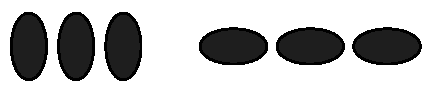
\includegraphics[width=0.6\columnwidth]{Figures/Introduction/Uniaxial_chains.pdf}
    \caption{Two possible chain geometries for uniaxial islands. \textbf{Left:} chain along the islands' hard axis. \textbf{Right:} chain along the islands' easy axis.}
    \label{fig:Intro_IslandEllipticChainGeometries}
\end{figure} \par
Suppose an initial situation as shown at the top of \cref{fig:Intro_SolitonRandomWalk}, where the wire has been initialized in a `1' state. Then all subsequent islands will prefer to be magnetized in alternating directions. Now the input bit is forcibly switched, so its magnetization points down, and we wish to propagate this signal through the wire, as shown on the second row of \cref{fig:Intro_SolitonRandomWalk}. The second magnetic moment then wants to align itself up due to its left neighbor (the input bit), but also wants to align itself down due to its right neighbor. As such, no net force acts on the second bit and it will randomly switch. Such a `defect' in the wire is called a magnetic soliton.~\cite{MQCA_RoomTemp} As soon as this second bit randomly changes to the `up' direction, the third bit is now in a similar situation, as shown at the bottom of \cref{fig:Intro_SolitonRandomWalk}, and the soliton has moved one island to the right. Now both the second and third bit have an equal chance of switching, and thus the signal has an equal chance of propagating forward to the output (third bit switches) or backward to the input (second bit switches). Thus, the signal (or, equivalently, the soliton) will perform a random walk along the wire. If the input bit is forced to remain `0', the signal will thus reach the output after a time proportional to the square of the number of nanomagnets in the chain, which is clearly not ideal.~\cite{Wolfram_RandomWalk} Several techniques have been proposed to force the signal to propagate along the wire in one direction.
\begin{figure}
    \centering
    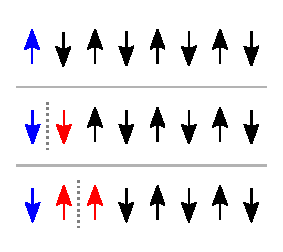
\includegraphics[width=0.5\columnwidth]{Figures/Introduction/Soliton_random_walk_2steps.pdf}
    \caption{Blue arrows are the input bits. Red arrows have no preferred direction due to competing interactions of their neighbors. A dotted line indicates the location of a magnetic soliton. \textbf{Top:} initial ordering of the wire for a `1' (up) input. \textbf{Middle:} input bit changes to `0' (down), causing no net force to act on the second island. \textbf{Bottom:} second island randomly switches, causing no net force to act on the third island anymore either.}
    \label{fig:Intro_SolitonRandomWalk}
\end{figure}
One technique makes use of additional biaxial anisotropy and an external magnetic field. The anisotropy is used to create a shallow energy minimum along the uniaxial anisotropy's hard axis. The biaxial anisotropy can be realized either by choosing a material with intrinsic magnetocrystalline biaxial anisotropy, or by modifying the shape of the island such that it exhibits biaxial anisotropy. The latter gives great control over the relative strength of the biaxial versus uniaxial anisotropy~\cite{SubnanosecondPropagation_AnisotropyChains}. The external field is used to initialize each island in this new shallow energy minimum, along what was previously known as the hard axis, whenever a new bit needs to be propagated, which can be seen as a form of clocking. Due to the shallow energy minimum, the magnetization will first stay along this hard axis until it is disturbed by any of its neighbors. The first island is initialized in either the `0' or `1' state and functions as the input bit. When the external field is removed, the second island will feel the input bit's dipole field, which will cause it to leave the shallow energy minimum and fall onto the easy axis. The third island then feels the second island falling in place, and so on. Thus, the signal successfully propagates in one direction.~\cite{NML_Carlton}
%When the external field is removed, each subsequent island chooses a direction to fall onto its easy axis. If this happens adiabatically, each island will fall in the correct antiparallel configuration and no solitons appear.~\cite{NML_Carlton}
\par
The use of an external magnetic field to reset the wire is not very `clean', because a global external field will affect all the wires in a given circuit. One possible solution is to manufacture the nanomagnetic islands such that each has a piezoelectric layer underneath, which can induce strain in the island, thus exerting a force on the magnetization (see \cref{par:Energy_MagnetoElastic}). Each nanomagnet can then be controlled electronically. Another possibility is to place the nanomagnetic islands between electrodes which produce a spin-polarized current. Through the spin transfer torque, these electrons can then exert a torque on the magnetization.~\cite{SwitchingForced_EnergyEfficient,syllabus_PoAEaPD} \par
By now it is clear why a chain along the hard axes (\cref{fig:Intro_IslandEllipticChainGeometries}, left) is preferred over a chain along the easy axes (\cref{fig:Intro_IslandEllipticChainGeometries}, right). In the latter case, when initializing the islands along their hard axes using an external field, they are being forced in a parallel configuration, while for such adjacent dipoles the minimal energy configuration is antiparallel. Without additional stabilizers as proposed in~\cite{NML_Carlton}, the signal propagation will thus be much more prone to random thermal errors.

\subsubsection{Biaxial}
\begin{figure}
    \centering
    
\includegraphics[width=0.5\columnwidth]{Figures/Introduction/Biaxial_chain.pdf}
    \caption{Minimal energy configuration of a balanced chain of biaxial nanomagnets. Blue arrow indicates the input island.}
    \label{fig:Intro_IslandBiaxialChainGeometry}
\end{figure}
The most straightforward way to transmit biaxial information is to use a nanowire in a similar manner as in the uniaxial case, where the biaxial islands are placed with their easy axes in an `XX' configuration. The lowest energy configuration of such an `XX' wire is shown in \cref{fig:Intro_IslandBiaxialChainGeometry}, where the blue island is once again the input. Because of the biaxial anisotropy, there are four possible directions for the magnetization of this input island. Due to the high degree of symmetry of this wire geometry, all four possible inputs have equal ground state energy, so the wire is perfectly balanced. This balancedness is also clear from the energy landscape in \cref{fig:two-islands_interaction_(r0.66_L100)_aPi4andPi4}, as explained in \cref{par:TwoIslands_InteractionAngle}. \par
This type of wire does, however, also hit the same problems with random walks. Unlike the uniaxial case, this can now no longer be resolved by initializing the islands in between the stable states such that they fall adiabatically to the energy minimum, because there are now four perpendicular stable states and it is hence impossible to force the magnetization in an initial direction that does not favor any of these four directions. \par
Note that, if one connects a wire to a logic gate, the logic gate will influence the wire as much as the wire will influence the logic gate. If the input or output nanomagnets of a logic gate are close to the nanomagnets responsible for the logic operation, adding a wire can cause the logic gate to stop functioning correctly. Hence, it can be advantageous to design logic gates in such a way that their inputs and outputs are already at the end of a short chain, such that increasing the wire length to connect it to another logic gate does not significantly influence their functioning.

\FloatBarrier
\subsection{Imaging the magnetization}
If one wishes to not only perform theoretical, but also practical studies on nanomagnetic islands, it can be useful to employ specialized microscopy techniques to image the magnetization direction. A small selection of often encountered techniques are presented in this section, each with certain advantages and disadvantages. Many other techniques besides those discussed below exist, like scanning electron microscopy with polarization analysis (SEMPA)~\cite{Imaging_SEMPA}, Lorentz microscopy~\cite{Imaging_Lorentz}, spin polarized scanning tunneling microscopies (SP-STM), superconducting quantum interference devices (SQUID) \dots Note that it is also possible to determine the average magnetization of a single island by adding electrodes and using effects from spintronics, though this can hardly be called an imaging technique, but rather a form of sensing.

\subsubsection{Magnetic Force Microscopy}
Magnetic Force Microscopy (MFM) is a form of scanning probe microscopy that can measure out-of-plane magnetic fields. For this, a cantilever with a magnetic tip is used which is scanned across the sample at a very low height. If this tip were to simply scan over the surface without keeping a small distance to the sample, both the magnetic forces as well as the atomic forces would be measured. To remedy this, the topography of the sample is first determined using conventional atomic force microscopy.~\cite{NML_Carlton, PEEM} Once the topography is known, the magnetic tip can scan the sample while maintaining a constant distance above it at any point using the now known topography. This decouples the measurement of magnetic forces from the atomic forces and allows one to determine only the magnetic field. Important to note is that the force measured is only the out-of-plane component of the magnetic field, because the cantilever can only move vertically and is thus only sensitive to the vertical component of the magnetic field.~\cite{NML_Carlton} One must also take care that the magnetic tip does not significantly influence the magnetization of the sample itself.~\cite{Probing_MagnetoOptics} \par
When imaging a nanomagnet, it will manifest itself in the output as the combination of a region with positive and a region with negative out-of-plane magnetic field, because the stray magnetic field of a dipole curls back on itself.~\cite{NML_Carlton} An example of an MFM image of a chain of nanomagnets is shown at the top of~\cref{fig:Intro_Imaging}. \par
The main disadvantage of MFM is that it does not image the magnetization directly, but rather the stray out-of-plane magnetic fields, which can make the results more difficult to interpret. It can however achieve a very high resolution due to its close resemblance to atomic force microscopy. Furthermore, it is a relatively cheap and commonly available technique compared to X-ray based techniques, which are discussed in the next section.

\subsubsection{X-ray Magnetic Circular Dichroism: PEEM and MTXM}
Both Photoelectron Emission Microscopy (PEEM) and Magnetic Transmission X-ray Microscopy (MTXM) are techniques which rely on a physical phenomenon called X-ray Magnetic Circular Dichroism (XMCD). This effect states that the number of electrons emitted from the sample upon irradiation with circularly polarized X-rays depends on the magnetization direction of the surface of the sample.~\cite{NML_Carlton} More specifically, the measured quantity is the angle $\theta$ between the magnetization direction $\vb{M(\vb{r})}$ of the sample and the photon spin $\vec{\sigma}$, which is aligned with the photon propagation direction and changes sign when the photon helicity is reversed.~\cite{PEEM} The intensity of emitted electrons is given by
\begin{equation}
    I_{\mathrm{XMCD}} \propto M_{sat} \cos(\theta) \mathrm{.}
    \label{eq:XMCD}
\end{equation} 
This way, the in-plane magnetization can be measured directly, which can make the results easier to interpret than an MFM image. To achieve high contrast, one can use X-rays with a frequency near an absorption edge.~\cite{SubnanosecondPropagation_AnisotropyChains} \par

Photoelectron Emission Microscopy (PEEM) images these secondary electrons emitted from the sample upon irradiation with X-rays. This kind of electron microscopy can achieve a high spatial resolution of less than \SI{50}{\nano\metre}, with a typical probing depth in metals of about \SI{2}{\nano\metre} due to the mean free path of the electrons, so PEEM is a surface sensitive technique. A slightly more detailed description of the geometry and image acquisition process of this kind of electron microscope can be found in~\cite{PEEM}. \par 

Magnetic transmission X-ray microscopy (MTXM) is a similar technique which also relies on XMCD. However, instead of detecting the number of emitted electrons as in PEEM, it is now the transmission of X-rays through the sample that is measured. The penetration depth of \SI{1}{\kilo\electronvolt} X-rays is about \SI{100}{\nano\metre}.~\cite{Imaging_MTXM} MTXM can be used to image the magnetization dynamics themselves on sub-nanosecond time scales; imaging as fast as \SI{100}{\pico\second} has been reported and used in literature and techniques for probing on femtosecond time scales are under research.~\cite{SubnanosecondPropagation_AnisotropyChains, Imaging_MTXM} \par

Besides the magnetization direction, also the chemical composition of the sample can be determined using the spectrum of emitted electrons or transmitted X-rays for PEEM and MTXM, respectively.~\cite{PEEM,Imaging_MTXM} Unfortunately, since XMCD requires circularly polarized X-rays, both imaging techniques require a synchrotron light source and corresponding equipment like helical undulators, which are only available at specialized institutes.

\begin{figure}
     \centering
     \begin{subfigure}[b]{0.8\textwidth}
         \centering
         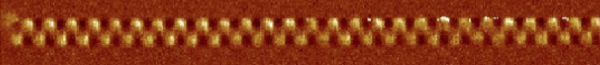
\includegraphics[width=\textwidth]{Figures/Introduction/NML_Carlton - Figure 1.15 cropped.png}
     \end{subfigure}
     \begin{subfigure}[b]{0.8\textwidth}
         \centering
         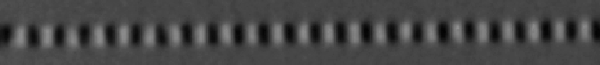
\includegraphics[width=\textwidth]{Figures/Introduction/NML_Carlton - Figure 1.17 cropped.png}
     \end{subfigure}
     \caption{Typical MFM (top) and PEEM (bottom) image of the same chain of elliptical nanomagnets placed along their hard axes (as in the left part of \cref{fig:Intro_IslandEllipticChainGeometries}), indicating that these two techniques are sensitive to different components of the magnetic field. Dark regions correspond to low measured values, light regions to high values. Figures taken from \cite{NML_Carlton}.}
     \label{fig:Intro_Imaging}
\end{figure}

\subsubsection{Magneto-Optical Kerr Effect}
The Magneto-Optical Kerr Effect (MOKE) is another physical phenomenon that can be used to determine the magnetization direction. A linearly polarized laser beam is focused onto the sample, and the polarization state of the reflected light is measured in order to access the longitudinal Kerr effect.~\cite{MQCA_RoomTemp} This effect states that, depending on the angle between the magnetization and the incoming light, the reflected light will become elliptically polarized to a certain degree.~\cite{KerrFaraday_book} The effect is small, but the ellipticity is directly proportional to the cosine of the angle, which can then be used to derive the magnetization direction. There also exists the transversal Kerr effect, though this is not often used as it results in a change in reflectivity, which is more difficult to detect and prone to error. \par
Due to the diffraction limit of the laser, MOKE-based techniques have a low resolution and can only measure the average magnetization over a larger area, on the order of several \si{\micro\metre\squared}. For structures smaller than this diffraction limit the signal strength diminishes.~\cite{Probing_MagnetoOptics} One must take care that the focused laser beam does not excessively heat up the sample, as this could influence the magnetization itself. The temperature rise for a \SI{2.5}{\milli\watt} laser focused on a \SI{5}{\micro\metre} diameter spot was however found to be negligible by Cowburn \textit{et al.}~\cite{Probing_MagnetoOptics} \par
This measurement technique can be easier or cheaper to set up than X-ray based techniques, but the (very) low resolution does not allow the imaging of individual nanomagnets in complex structures.

\clearpage
\section{Physics}
In a crystalline material, the atoms are evenly spaced. Each atom has a discrete magnetic moment $\vb{m_i}$ associated with it. The interaction of these many magnetic moments can give rise to macroscopic effects. Since every magnetic moment interacts with every other magnetic moment, the underlying problem is a discrete N-body problem. Unfortunately, such a problem quickly becomes very hard if not impossible to solve analytically for even very few bodies, hence restricting analytical calculations to very small systems.~\cite{abert2013discrete} Due to the lack of an analytical solution, many particular problems can only be solved approximately in a numerical manner.~\cite{abert2013discrete} Even with numerical techniques, the computational power or time required to solve an N-body problem increases rapidly for an increasing amount of bodies, due to the number of interactions. \par
For this reason, a continuum theory was developed, called the \textbf{micromagnetic theory}. In this formalism, the magnetization is represented by the continuous magnetization field, denoted by $\vb{M}(\vb{r}) = M_{sat} \vb{m}(\vb{r})$. This is the magnetic moment per unit volume averaged over a small region of space, with $M_{sat}$ [\si{\ampere\per\metre}] called the saturation magnetization.~\cite{Gilbert1956} $\vb{m}(\vb{r})$ is a unit vector field called the reduced magnetization, which should not be confused with the individual magnetic moments $\vb{m_i}$. $\vb{M}(\vb{r})$ has constant norm because of the even spacing of atoms in the crystal structure.~\cite{abert2013discrete}
The size of this small region is characterized by the exchange length $\lambda$, a formula for which is given by \cref{eq:Energy_ExchangeEnergy_ExchangeLength}. It should be much smaller than the size of a single magnetic domain, yet much larger than a crystal unit cell, so on the order of several nanometres. It is clear that this continuum approximation is only applicable if locally all discrete magnetic moments try to align themselves parallel to each other, i.e.
\begin{equation}
    \vb{m_i} \approx \vb{m_j}~~\mathrm{if}~~\abs{\vb{r_i} - \vb{r_j}} < \lambda \mathrm{,}
\end{equation}
as is for example the case in ferromagnets.~\cite{abert2013discrete} \par
In situations where this approximation holds, the continuum theory can provide a significant computational improvement, because one can now use a finite difference approach with typical cell sizes on the order of $\lambda$. This significantly decreases the amount of variables compared to the original N-body problem, where every single atom had to be taken into account. The usual size of a simulation using micromagnetic theory is on the order hundreds of nanometres, using millions of cells with dimensions on the order of $\lambda$.~\cite{abert2013discrete} \par
Thus, the micromagnetic theory works well on a microscopic scale and can be solved numerically in a reasonable amount of time, which would be wholly impossible with an N-body approach.

\subsection{Energy contributions}
The energy corresponding to a static configuration of the reduced magnetization field $\vb{m}(\vb{r})$ is the sum of several different contributions
\begin{equation}
    E = E_{exch} + E_{anis} + E_{demag} + E_{Zeeman} + E_{me} \mathrm{.} \label{eq:Energy_Terms}
\end{equation}
The physical nature of these different terms along with small derivations to accomodate them to the continuum approximation are presented in this section.
\subsubsection{Exchange energy}
\label{par:Energy_Exchange}
The exchange energy is of quantum mechanical origin. It tries to align neighboring spins and takes on the simple form
\begin{equation}
    E_{i,j} = -J_{ij} \vb{S_i} \vdot \vb{S_j} \mathrm{.}
    \label{eq:Energy_ExchangeEnergy_Discrete}
\end{equation}
Summing over all contributions gives
\begin{equation}
    E = -\sum_{i,j} J_{ij} S^2 \vb{n_i} \vdot \vb{n_j} \mathrm{,}
    \label{eq:Energy_ExchangeEnergy_SumDiscrete}
\end{equation}
with $\vb{S_i} = S \vb{n_i}$ and $\abs{n_i} = 1$. 
The sign of $J$ determines whether the spins align parallel ($J>0$) or anti-parallel ($J<0$). A parallel alignment results in a so-called ferromagnetic material, while an anti-parallel alignment is characteristic of an anti-ferromagnetic material. \par
Micromagnetic theory makes use of the magnetization field $\vb{m}(\vb{r})$, while \cref{eq:Energy_ExchangeEnergy_Discrete} is discrete. An equation similar to \cref{eq:Energy_ExchangeEnergy_SumDiscrete}, but for the continuous $\vb{m}(\vb{r})$, can now be written down:
\begin{equation}
    E_{exch} = \int_\Omega \sum_i A_i \vb{m}(\vb{r}) \cdot \vb{m}(\vb{r} + \Delta\vb{r}_i) \mathrm{.} \label{eq:Energy_ExchangeEnergy_SumContinuous}
\end{equation}
Since two particles $i$ and $j$ only feel the exchange interaction when they are close to each other, $\vb{m}(\vb{r}) \cdot \vb{m}(\vb{r} + \Delta\vb{r})$ can be expanded in first order~\cite{abert2013discrete} to
\begin{align*}
    \vb{m}(\vb{r}) \cdot \vb{m}(\vb{r} + \Delta\vb{r}) &= 1 - \frac{1}{2}(\vb{m}(\vb{r}) - \vb{m}(\vb{r} + \Delta\vb{r}))^2 \\
    &\approx 1 - \frac{1}{2}\sum_i(\Delta\vb{r} \cdot \gradient{m_i})^2 \label{eq:Energy_ExchangeEnergy_DotApprox} \mathrm{.}
\end{align*}
This can be substituted into \cref{eq:Energy_ExchangeEnergy_SumContinuous}~\cite{abert2013discrete,Gilbert1956}, finally yielding
\begin{equation}
    E_{exch} = A_{ex} \int_\Omega \sum_i (\gradient{m_i}(\vb{r}))^2 \, d\vb{r} \mathrm{.} \label{eq:Energy_Term_Exchange}
\end{equation}
$A_{ex}$ is called the exchange stiffness constant.~\cite{Gilbert1956} The physical interpretation of this energy term is that the magnetization tries to align itself as smoothly as possible.
The exchange length $\lambda$, which characterizes the length scale over which the magnetization can still be approximated as nearly uniform, is defined in SI units \cite{ExchangeLength, ExchangeLength_original, MuMax3} as
\begin{equation}
    \lambda = \sqrt{\frac{2 A_{ex}}{\mu_0 M_{sat}^2}} \mathrm{.}
    \label{eq:Energy_ExchangeEnergy_ExchangeLength}
\end{equation}
It can be used as a rule of thumb for the cell size of micromagnetic simulations, which should be smaller than $\lambda$ such that sampling at that length scale is sufficient to capture all relevant details.~\cite{ExchangeLength}

\subsubsection{Anisotropy energy}
A material may exhibit anisotropy due to its crystal structure. The most often encountered types of anisotropy are uniaxial and cubic anisotropy. Uniaxial anisotropy is common in hexagonal or tetragonal crystal structures, while cubic anisotropy is often present in FCC or BCC structures.~\cite{Gilbert1956, abert2013discrete} \par
In the uniaxial case, the energy is minimal when the magnetization lies along a certain axis $\vb{u}$. In the cubic case, there are three such axes $\vb{e_i}, i=1,\dots,3$, which are all equivalent. The direction of $\vb{M}$ along this axis (i.e. $\vb{m}=\pm \vb{u}$) does not matter, such that $E(\vb{m}_{min}) = E(-\vb{m}_{min})$. For this reason, only even orders in the Taylor expansion are considered.~\cite{abert2013discrete} For uniaxial anisotropy this gives
\begin{equation}
    E_{anis,u} = - \int_\Omega \big(K_{u1} (\vb{m} \cdot \vb{u})^2 + K_{u2} (\vb{m} \cdot \vb{u})^4 + \dots\big) \, d\vb{r} \mathrm{.} \label{eq:Energy_Term_AnisUniaxial}
\end{equation}
The coefficients $K_{ui}$ [\si{\joule\per\metre\squared}] are called the uniaxial anisotropy constants.
For cubic anisotropy, one can use a similar symmetry reasoning~\cite{abert2013discrete} to find
\begin{equation}
    E_{anis,c} = \int_\Omega \big(K_{c1} (m_1^2m_2^2 + m_2^2m_3^2 + m_3^2m_1^2) + K_{c2} m_1^2m_2^2m_3^2\big) \, d\vb{r} \mathrm{,} \label{eq:Energy_Term_AnisCubic}
\end{equation}
with $m_i(\vb{r}) = \vb{m}(\vb{r}) \cdot \vb{e_i}, i=1,\dots,3$.

\subsubsection{Demagnetization energy/Magnetostatic energy}
The demagnetization energy, often also called the magnetostatic energy, is the energy arising from the interaction of every magnetic moment in a ferromagnetic material with the force of every other magnetic moment in the material.~\cite{NML_Carlton} In other words, it is the energy of the magnetization in the magnetic field created by itself.~\cite{abert2013discrete}
From classical electrodynamics it is known that, in the absence of currents,
\begin{align}
	\div{\vb{B}} &= 0 \label{eq:Energy_Demag_DivB0} \\
	\curl{\vb{H}} &= 0 \label{eq:Energy_Demag_CurlH0} \\
	\vb{B} &= \mu_0 (\vb{H} + \vb{M}) \label{eq:Energy_Demag_BHM} \mathrm{.}
\end{align}
From \cref{eq:Energy_Demag_CurlH0} immediately follows that $\exists \psi(\vb{r}): \vb{H} = -\gradient{\psi}$. By substituting \cref{eq:Energy_Demag_BHM} in \cref{eq:Energy_Demag_DivB0} it is then clear that
\begin{equation}
    \laplacian{\psi} = \div{\vb{M}} \mathrm{.}
\end{equation}
The solution of this Laplace equation, for the boundary condition $\abs{\vb{r}} \rightarrow 0 \Rightarrow \psi \rightarrow 0$, is found using Green's function and Green's theorem:
\begin{align*}
    \psi(\vb{r}) &= -\frac{1}{4\pi}\int_\Omega \frac{\boldsymbol{\nabla'\,\vdot}\,\vb{M}(\vb{r'})}{\abs{\vb{r}-\vb{r'}}} \,d\vb{r'} + \frac{1}{4\pi}\int_{\partial\Omega} \frac{\vb{M}(\vb{r'}) \vdot \vb{n}}{\abs{\vb{r}-\vb{r'}}} \,d\vb{s'} \\
    &= \frac{1}{4\pi}\int_\Omega \vb{M}(\vb{r'}) \vdot \boldsymbol{\nabla'} \frac{1}{\abs{\vb{r}-\vb{r'}}} \,d\vb{r'} \mathrm{.}
\end{align*}
A more rigorous derivation is given in~\cite{abert2013discrete}.
From this explicit expression for $\psi(\vb{r})$, one can determine $\vb{H_{demag}} = -\gradient{\psi}$. The energy can then also be found through classical electrodynamics as
\begin{equation}
    E_{demag} = -\frac{\mu_0}{2} \int_\Omega \vb{M} \cdot \vb{H_{demag}} \, d\vb{r} \mathrm{.} \label{eq:Energy_Term_Demag}
\end{equation}
There is an additional $\frac{1}{2}$ factor because each interaction is counted twice.

\subsubsection{Zeeman energy}
If an external field is applied, an additional energy term similar to the demagnetization energy appears, but now without the factor $\frac{1}{2}$ because the interaction comes from an external source:
\begin{equation}
    E_{Zeeman} = -\mu_0 \int_\Omega \vb{M} \vdot \vb{H_{ext}} \, d\vb{r} \mathrm{.} \label{eq:Energy_Term_Zeeman}
\end{equation}

\subsubsection{Magneto-elastic energy}
\label{par:Energy_MagnetoElastic}
In case there is stress present in the crystal lattice, an additional magneto-elastic energy term can be formulated~\cite{Gilbert1956}. For an isotropic material this is given by
\begin{equation}
    E_{me} = B \int_\Omega \sum_{i,j} m_i m_j \frac{\partial s_i}{\partial x_j} \,d\vb{r} \mathrm{,}
\end{equation}
with $\vb{s}(\vb{r})$ the displacement field of the lattice.

\subsubsection{Other energy terms}
Other energy terms still exist to describe other specific phenomena, though these will not be used in this work. An example of such an energy term is the Dzyaloshinskii-Moriya interaction~\cite{DzyaloshinskiiMoriya}, which tries to orient neighboring spins perpendicular to each other, and is responsible for the stabilisation of skyrmions as described in~\cite{skyrmions}.

\subsection{Landau-Lifschitz-Gilbert equation}
The aforementioned energy terms express the potential energy of a static magnetization state $\vb{m}(\vb{r})$, but do not tell us how this magnetization evolves over time. Landau and Lifschitz~\cite{lifdau} first described the time evolution of the magnetization field, as the sum of a precessional and a damping term.~\cite{abert2013discrete, NML_Carlton, phd_leliaert} The Landau-Lifschitz (LL) equation reads
\begin{equation}
    \frac{\partial \vb{m}}{\partial t} = - \gamma_0' \vb{m} \cross \vb{H_{eff}} - \alpha' \vb{m} \cross (\vb{m} \cross \vb{H_{eff}}) \mathrm{.}
    \label{eq:LL}
\end{equation}
\begin{figure}
    \centering
    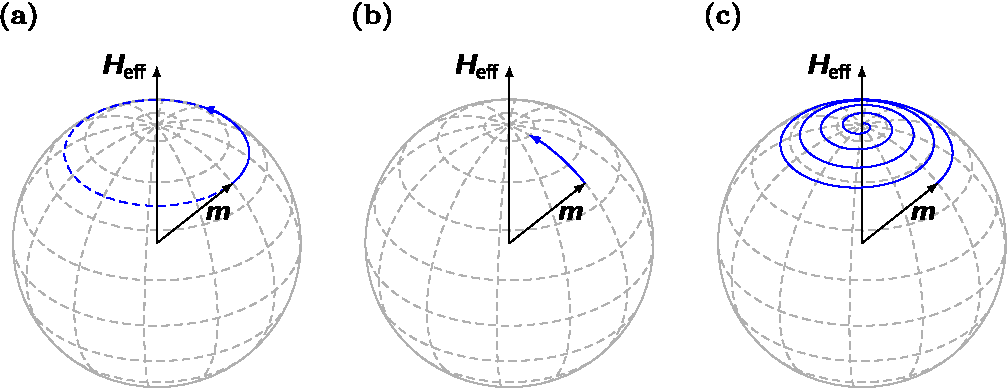
\includegraphics[width=0.9\columnwidth]{Figures/Introduction/abert2013discrete - Figure 2.2.pdf}
    \caption{Motion of a magnetic moment as described by the LLG equation. The motion can be divided into the \textbf{(a)} precessional and \textbf{(b)} damping components. \textbf{(c)} Resulting motion including both precession and damping. Figure taken from~\cite{abert2013discrete}.}
    \label{fig:LLG_motion_Heff}
\end{figure}
\par The meaning of both terms and their sum is illustrated in \cref{fig:LLG_motion_Heff}. The first term $\vb{m} \cross \vb{H_{eff}}$ describes the precession of the magnetization around the effective field and can be derived from quantum mechanical considerations. The second term $\vb{m} \cross (\vb{m} \cross \vb{H_{eff}})$ was introduced phenomenologically, to make sure the precession does not carry on forever, and causes $\vb{m}$ to slowly damp toward the effective field vector $\vb{H_{eff}}$.~\cite{NML_Carlton} The effective field $\vb{H_{eff}}$ is defined as
\begin{equation}
	\vb{H_{eff}} = - \frac{1}{\mu_0} \frac{\partial E}{\partial \vb{M}} \mathrm{,}
	\label{eq:H_eff}
\end{equation}
with the energy $E$ the sum of several contributions as explained before. $\partial E/\partial \vb{m}$ means the vector whose components are $\partial E/\partial m_x$, etc.~\cite{ThermFluc_SingleDomain} Some reasons for the phenomenological damping are eddy currents, or spin-lattice coupling.~\cite{phd_leliaert} These are rather macroscopic explanations, which do not tell us anything about the fundamental origin of damping.
\par
In order to obtain a physically more intuitive damping term, Gilbert~\cite{Gilbert1955ALF} proposed an alternative form of the LL equation. He argued that, because $\vb{m}(\vb{r})$ is always a unit vector, its motion can be described by that of a rotating body, thus allowing the use of a Lagrangian formalism to determine the dynamics of the system.~\cite{abert2013discrete} For the kinetic energy term in this Lagrangian, he proposed $-M_{sat}/\gamma \dot{\phi} \cos(\theta)$, with $\phi$ and $\theta$ spherical coordinates and the diacritic overdot denoting a time derivative, thus relating the damping to the time derivative of the magnetization.~\cite{abert2013discrete} This yields the Landau-Lifschitz-Gilbert (LLG) equation~\cite{ThermFluc_SingleDomain, phd_leliaert, LEL-17b}
\begin{equation}
    \frac{\partial \vb{m}}{\partial t} = - \gamma_0 \vb{m} \cross \vb{H_{eff}} + \alpha \vb{m} \cross \frac{\partial \vb{m}}{\partial t} \mathrm{.}
    \label{eq:LLG}
\end{equation}
Here, $\gamma_0=\mu_0 \gamma$ with $\gamma$ the gyromagnetic ratio. The dimensionless $\alpha > 0$ is called the Gilbert damping constant, and is for example equal to 0.01 for permalloy. The precession frequency in absence of damping, also called the Larmor frequency, is given by  $f_L=\frac{\gamma_0}{2\pi}\abs{\vb{H_{eff}}}$.~\cite{phd_leliaert} 
It is also possible to derive the LLG equation as a limit case of a quantum mechanical description of a spin subject to the effects corresponding to the different energy terms.~\cite{abert2013discrete,bode2012current}
Using the differential form, Hickey \textit{et al.} derived the damping from first-principles~\cite{hickey2009origin}, with the intrinsic origin of the damping being spin-orbit coupling, due to relativistic corrections to the Hamiltonian which couple the spin to the electric field.~\cite{hickey2009origin} This yields an explicit expression for the damping constant $\alpha$ as a function of several fundamental constants and material parameters. \par
Though the LL and LLG equations look slightly different, they can easily be transformed into each other~\cite{ThermFluc_SingleDomain,phd_leliaert} using the substitutions
\begin{align*}
    \gamma_0' &= \frac{\gamma_0}{1+\alpha^2} \\
    \alpha' &= \alpha \frac{\gamma_0}{1+\alpha^2} \mathrm{.}
\end{align*}
By applying these substitutions, the first term in the LL equation~\eqref{eq:LL} governing the precession frequency becomes dependent on the damping constant $\alpha$, which is the physically correct behavior.~\cite{phd_leliaert} This is, however, a purely academic consideration, as in realistic situations the damping constant is small enough for this effect to be negligible. \par
Additional torques can also be taken into account, like the Zhang-Li or Slonczewski spin-transfer torques, which describe the interaction between a spin-polarised current and the magnetization~\cite{ZhangLiSpinTransferTorque, MuMax3, syllabus_PoAEaPD}. This effect can for example be used, among many other applications, in information storage technologies like MRAM and magnetic field sensors.~\cite{syllabus_PoAEaPD}


\subsubsection{Numerical solution}
The micromagnetic theory described above makes abstraction of the individual atomic magnetic moments $\vb{m}_i$ in favor of a continuum theory $\vb{m}(\vb{r})$ to describe ferromagnetic materials. The time evolution of this theory is described by the Landau-Lifschitz equation \eqref{eq:LL}, which provides an explicit form for the time derivative of the magnetization. For this reason, the LL equation is preferred over the LLG equation \eqref{eq:LLG} in numerical solvers, as the latter is implicit. For most geometries, an analytical solution is very hard or even impossible to write down, so one has to resort to numerical approximations of the micromagnetic theory, like a finite difference (FD) discretization. \par
For this thesis, \mumax{}~\cite{MuMax3} will be used. This is a GPU-accelerated micromagnetic simulation program developed at the DyNaMat group of Ghent University. It calculates the space- and time-dependent magnetization dynamics in nano- to micro-sized ferromagnets using a finite-difference discretization, which is well suited for the problems considered in this thesis. By computing on the graphics processing unit (GPU), the finite difference scheme can be solved in parallel, significantly speeding up the calculation with respect to serial codes.~\cite{MicromagneticGPU} \par
In order to perform a simulation, \mumax{} makes use of user-written input files, which give a lot of freedom to said user. One first defines the cell size of the finite difference grid, and the geometry $\Omega \subset \mathbb{R}^3$ of the ferromagnetic material. Multiple regions $\Omega_i$ can also be defined, which will prove useful when considering multiple nanomagnetic islands, as this allows for quantities to be calculated for each island separately. One can then initialize the magnetization $\vb{m}(\vb{r})$ throughout the geometry. In this thesis, often a uniform magnetization $\vb{m}(\vb{r}) = \vb{a}, \forall \vb{r} \in \Omega_i$ is used as the initial state. Once the magnetization has been initialized, there are two functions to allow the magnetization profile to settle to the geometry, in order reach the local energy minimum. The first option is to \code{relax()} the magnetization. The function \code{minimize()} achieves the same, but takes larger steps and is therefore faster but more prone to reaching an incorrect result. Finally, one can run the simulation for a given time in presence of thermal fluctuations, which will be discussed in the next section. \par
There are still many more micromagnetic features available in \mumax{}, though these are not relevant to this thesis. A more detailed description of the design of \mumax{} is available in reference~\cite{MuMax3}.

\subsubsection{Thermal fluctuations}
The LLG equation only takes into account the fundamental physics of the magnetization dynamics at zero temperature. However, in our universe things exist at nonzero temperatures, and thermal fluctuations play an important role in magnetic logic devices, for example for reverse calculations. In order to simulate nanomagnetic structures at nonzero temperatures, Brown~\cite{ThermFluc_SingleDomain} developed a theory to model thermal fluctuations in single-domain particles, by adding a stochastic thermal field $\vb{H_{therm}}$ to the effective field $\vb{H_{eff}}$ in the LLG equation. This thermal field has to fulfill certain statistical properties, namely
\begin{align*}
    \langle \vb{H_{therm}} \rangle &= 0 \mathrm{,} \\
    \langle H_{therm,i}(t) H_{therm,j}(t') \rangle &= q \delta(t-t') \delta_{ij} \mathrm{,}
\end{align*}
where $q=(2 k_B T \alpha)/(M_{sat} \gamma_0 \mu_0 V)$, with $V$ the volume of the single-domain particle.~\cite{phd_leliaert} The angled brackets denote either a time average or correlation. With these random and uncorrelated properties of the time-dependent additional field term, the LLG equation becomes a Langevin equation.~\cite{ThermFluc_SingleDomain} However, a nanomagnetic island is not a perfect single-domain particle with uniform magnetization, and different nanomagnetic islands can influence each other through magnetostatic interactions.
Lyberatos~\cite{Lyberatos_1993} realized that every finite-difference cell in a numerical simulation can be seen as one such a single-domain particle, for which Brown's theory can then be applied.~\cite{phd_leliaert} More specifically, the thermal field was implemented in \mumax{}~\cite{LEL-17b,MuMax3} as
\begin{equation}
    \vb{H_{therm}} = \vec{\eta} \sqrt{\frac{2 \alpha k_B T}{M_{sat} \gamma_0 \mu_0 V \Delta t}} \mathrm{,}
    \label{eq:H_therm}
\end{equation}
where $\vec{\eta}$ is a random vector, determined from a standard normal distribution, whose value is changed after every time step. This equation is such that the thermal fluctuations are independent of the spatial discretization (volume $V$ and time step $\Delta t$) used.
There are many finite-difference solvers available in \mumax{}, for example different orders of Runge-Kutta solvers, some of which benefit from the first-same-as-last (FSAL) property. In such solvers, the last torque evaluation of the current step is the same as the first evaluation of the next step, which allows an increase in efficiency because this step only has to be evaluated once. However, the stochastic thermal field is not constant, and hence these solvers can no longer benefit from the FSAL property when thermal fluctuations are present.~\cite{LEL-17b} Another complication is that the time step $\Delta t$ appears in the expression for $\vb{H_{therm}}$. Since some solvers in \mumax{} improve their efficiency by using an adaptive time step, one must take additional care that the thermal field is calculated correctly. A detailed description of the implementation of the stochastic thermal field in \mumax{} is given in~\cite{LEL-17b}.

\clearpage
\section{Biaxial island}
\label{par:Biaxial_island}
The first part of this thesis consists of investigating the properties of a single biaxial island, as this will be the fundamental building block of more complex circuits. As thermal fluctuations play a big role in nanomagnetic logic, the energy barrier between stable states is important to investigate. The geometry of an island is one of the main factors determining this energy barrier. The geometry used throughout this thesis is the union of two identical perpendicular ellipses, as depicted in \cref{fig:biaxial_island:geometryTypical}, where \SI{0}{\degree} is defined as the direction pointing to the right, as usual in mathematics. When using the words `horizontal', `vertical' and `diagonal' in the context of a biaxial island, this will always be in reference to this figure. This geometry was chosen because it should be reasonably easy to manufacture due to the lack of sharp corners, as opposed to for example a geometry made of rectangles. It has two `degrees of freedom', namely the long and short axis of the ellipse. As the geometry has 4 symmetry axes, for a single island it is sufficient to consider angles from \SIrange{0}{45}{\degree}, though for clarity the figures will show from \SIrange{0}{90}{\degree}. \par
We will define the \textit{roundness} $\rho$ as the ratio of the short over the long axis of the ellipses, and the overall \textit{size} $L$ as simply being equal to the long axis. For example, $(\rho, L)=(0.55, \SI{100}{\nano\metre})$ indicates that the long axis of each ellipse is \SI{100}{\nano\metre} while the short axis is \SI{55}{\nano\metre}, as in the figure. \par
Furthermore, the in-plane angles of several quantities will be used: $\Theta$ denotes the instantaneous average magnetization angle, and its tilde counterpart $\widetilde{\Theta}$ the angle of the magnetization when it is relaxed to a local energy minimum. The angle of an external field is denoted by $\chi$, while its tilde counterpart $\widetilde{\chi}$ indicates a `virtual' external field, which is to be explained later. Finally, $\Phi$ denotes the angle by which the geometry of a biaxial island was rotated, i.e. the angle between its ellipse axes and the numerical Cartesian grid of the simulation domain.
\begin{figure}
    \centering
    
\includegraphics[width=0.3\columnwidth]{Figures/biaxial_island/Geometry/geomPlus55.png}
    \caption{Typical geometry of the biaxial island under investigation, in this specific case for $55\cross\SI{100}{\nano\metre}$ ellipses, i.e. $(\rho, L)=(0.55, \SI{100}{\nano\metre})$. White represents ferromagnetic material, black is free space.}
    \label{fig:biaxial_island:geometryTypical}
\end{figure}

\subsection{Energy barrier}
\label{par:Biaxial_EnergyBarrier}
Due to symmetry reasons, all of $\Theta = k\frac{\pi}{4} , k\in\mathbb{Z}$ are equilibria. However, not all are stable; some are energy minima while some are energy maxima. To determine the energy barrier $E_{barrier}$ between stable states, the energy landscape as a function of magnetization angle must be calculated. Important to note is that, if one simply sets the magnetization $\vb{M}$ of the entire island uniformly in one specific direction and calculates the energy, one finds that the energy is the same for all directions. This is due to the absence of the demagnetization field caused by the shape anisotropy of the magnetic geometry.~\cite{Nonmonotonic_reversal} Thus, if one wants to meaningfully calculate the energy landscape, the magnetization should first be relaxed to accommodate for the shape of the island. This is done using the \mumax{} command \code{minimize()}. However, simply doing so would result in a complete relaxation to an energy minimum, hence not yielding any useful information on the energy barrier, which is the difference between an energy minimum and maximum. To circumvent this issue, an external magnetic field is applied to keep the average magnetization $\frac{1}{A}\int_A \vb{M}\,dA$ close to the desired direction. Practically, this \textit{`virtual' external field} $\vb{B_{ext,v}}$ is realized through the custom field functionality in \mumax{}, using \code{AddFieldTerm} and \code{AddEdensTerm}. \par
The procedure is therefore as follows. First, the magnetization of the entire island $\vb{M}$ is initialized uniformly under an angle $\Theta$, and an external magnetic field $\vb{B_{ext,v}}$ is applied along that same direction. Then, the magnetization is relaxed using \code{minimize()}. The internal energy, responsible for the energy landscape, is then equal to $E_{total} - E_{Zeeman}$. This procedure to determine the internal energy is repeated for different angles $\Theta$ to generate an energy landscape from which the energy barrier can be deduced.

\subsubsection{Optimal virtual external field magnitude}
The procedure as described above makes use of an external magnetic field. This is merely out of necessity to make sure that a magnetization initialized in an unstable maximum energy state stays there and does not relax to the energy minimum, which would prevent the determination of the height of the energy barrier. In reality, there is no such field, so this `virtual' external field should ideally be of small magnitude. To investigate the influence of this magnitude on the energy landscape, a simulation was carried out in which both the angle and the magnitude of the external magnetic field were varied. In \cref{fig:barrierLandscape-sweepBext_r0.65}, the magnitude of the external magnetic field $\abs{\vb{B_{ext,v}}}$ was varied, with the angle $\widetilde{\chi}$ of this field taken at 64 equally spaced values from \SIrange{0}{90}{\degree}. For each of these values, a point is plotted showing the relaxed magnetization angle $\widetilde{\Theta}$ and the corresponding energy. Note that the average relaxed magnetization angle $\widetilde{\Theta}$ is not necessarily equal to the external magnetic field angle $\widetilde{\chi}$, as the relaxation process will tend to more or less cant the magnetization towards the closest intrinsic energy minimum. \par

\begin{figure}
     \centering
     \begin{subfigure}[b]{0.8\textwidth}
         \centering
         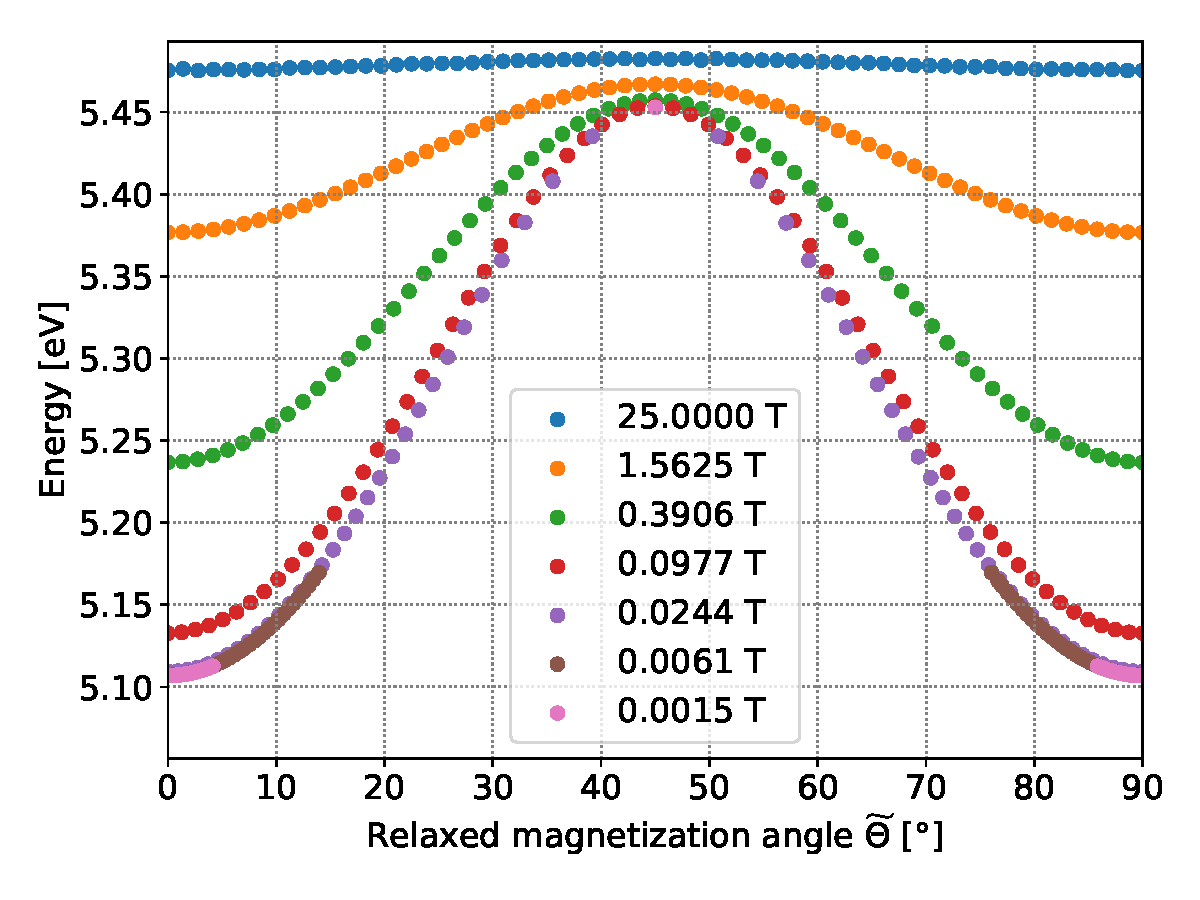
\includegraphics[width=\textwidth]{Figures/biaxial_island/BarrierLandscape/Plus_65_B25-0.001-div4_a128Pi_plotOptimized.pdf}
         \caption{$(\rho, L)=(0.65, \SI{100}{\nano\metre})$}
         \label{fig:barrierLandscape-sweepBext_r0.65}
     \end{subfigure}
     \begin{subfigure}[b]{0.8\textwidth}
         \centering
         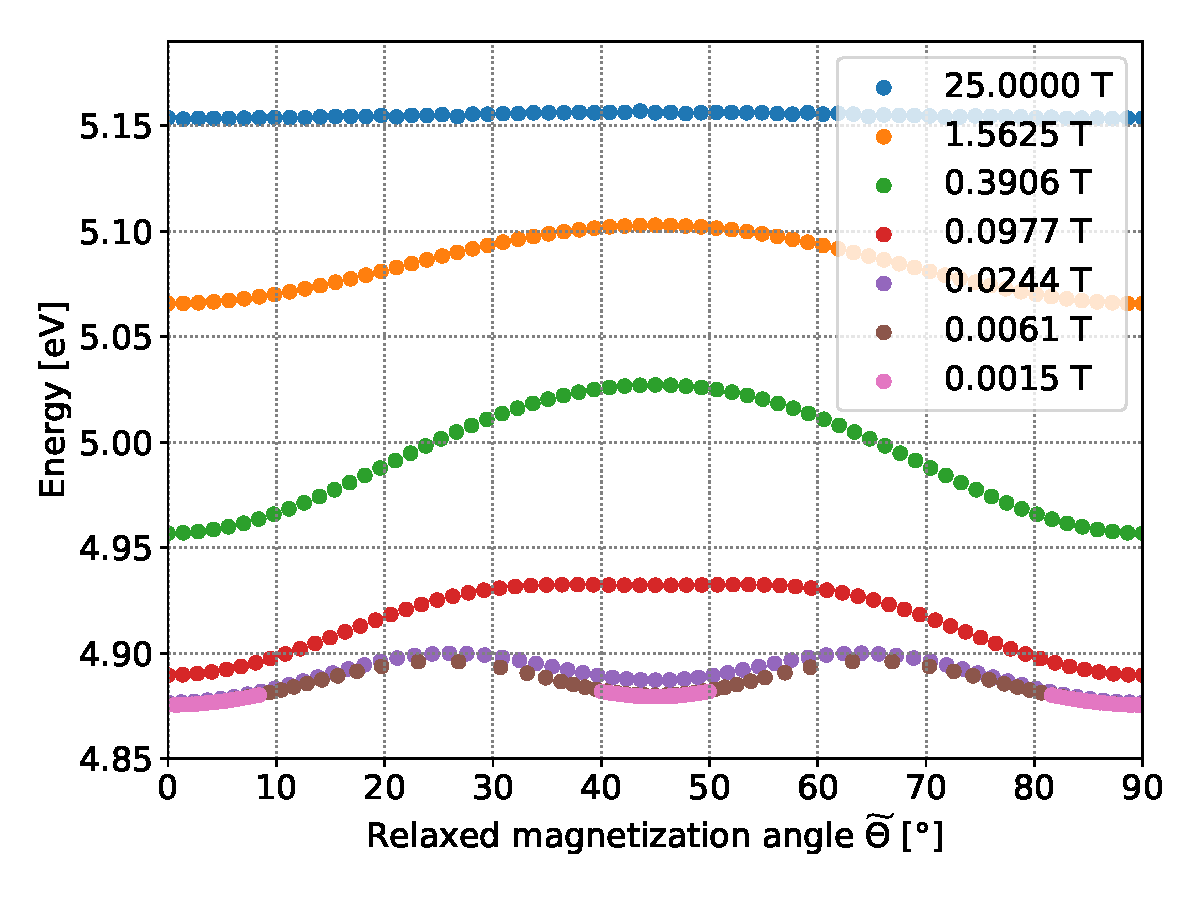
\includegraphics[width=\textwidth]{Figures/biaxial_island/BarrierLandscape/Plus_48.2_B25-0.001-div4_a128Pi_plotOptimized.pdf}
         \caption{$(\rho, L)=(0.482, \SI{100}{\nano\metre})$}
         \label{fig:barrierLandscape-sweepBext_r0.482}
     \end{subfigure}
    \caption{Energy landscape for two different geometries, calculated using various external magnetic field magnitudes $\abs{\vb{B_{ext,v}}}$ as shown in the legend. The external field angle $\widetilde{\chi}$ was varied uniformly in 64 steps from \SIrange{0}{90}{\degree}, for each magnitude, each dot corresponding to one such angle. The horizontal axis denotes the average magnetization angle $\widetilde{\Theta}$ after relaxation. Note that this is not necessarily equal to the external field angle, especially for low field magnitudes.}
    \label{fig:barrierLandscape-sweepBext}
\end{figure}

% \begin{figure}
%     \centering
%     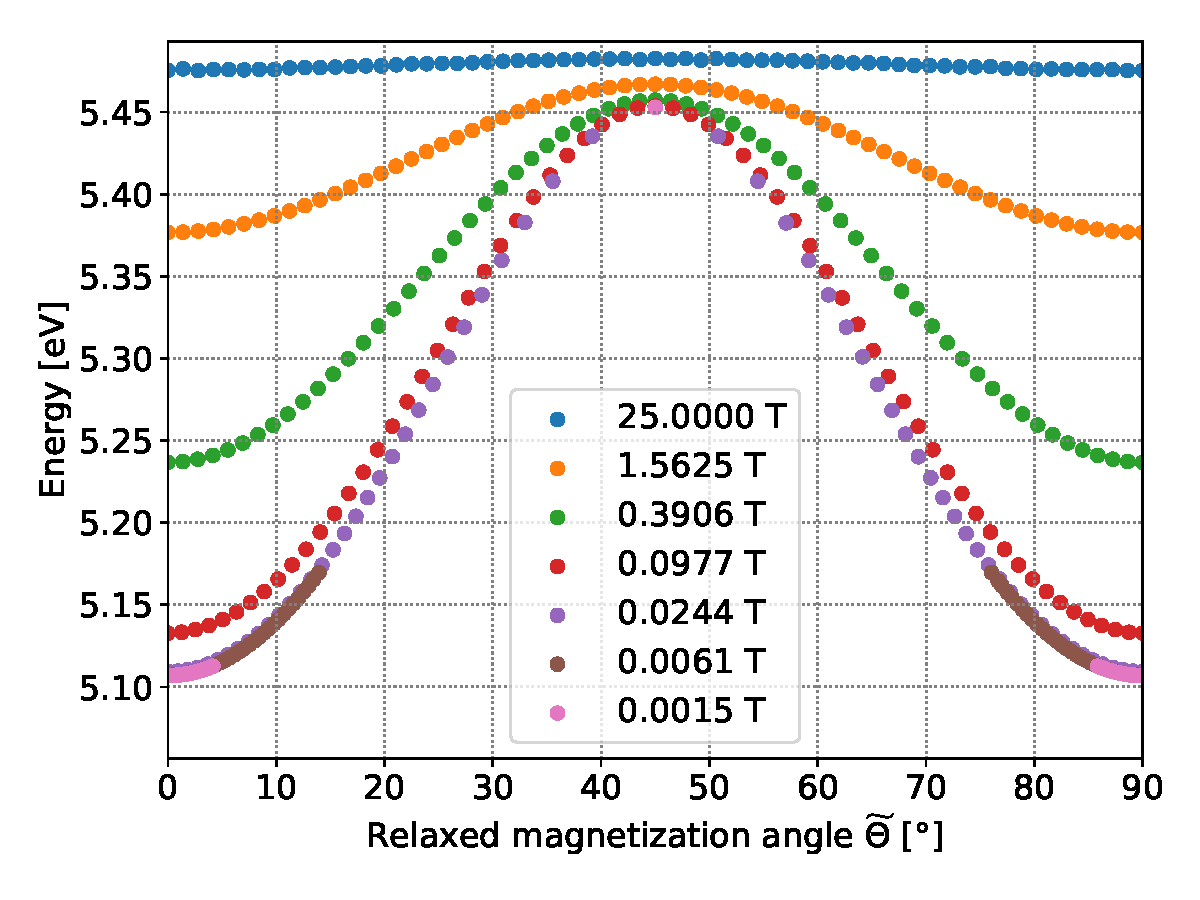
\includegraphics[width=0.9\textwidth]{Figures/biaxial_island/BarrierLandscape/Plus_65_B25-0.001-div4_a128Pi_plotOptimized.pdf}
%     \caption{Energy landscape for a $(\rho, L)=(0.65, \SI{100}{\nano\metre})$ geometry, calculated using various external magnetic field magnitudes $\abs{\vb{B_{ext,v}}}$ as shown in the legend. The external field angle $\widetilde{\chi}$ was varied uniformly in 64 steps from \SIrange{0}{90}{\degree}, for each magnitude, and each dot corresponds to one such angle. The horizontal axis denotes the average angle $\widetilde{\Theta}$ of the magnetization over the whole island after relaxation. Note that this is not necessarily equal to the external field angle, especially for low field magnitudes.}
%     \label{fig:barrierLandscape-sweepBext_r0.65}
% \end{figure}
% \begin{figure}
%     \centering
%     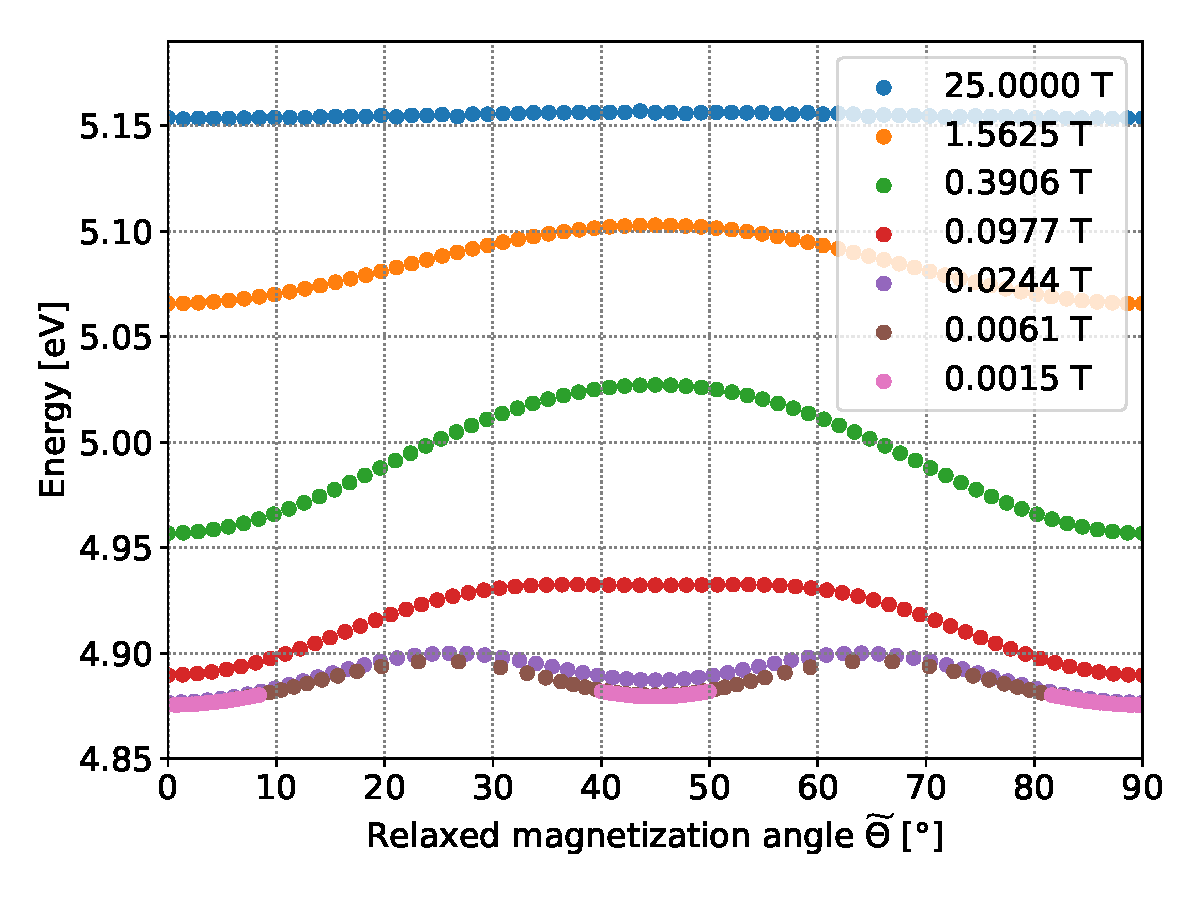
\includegraphics[width=0.9\textwidth]{Figures/biaxial_island/BarrierLandscape/Plus_48.2_B25-0.001-div4_a128Pi_plotOptimized.pdf}
%     \caption{Energy landscape for a $(\rho, L)=(0.482, \SI{100}{\nano\metre})$ geometry, calculated using various external magnetic field magnitudes $\abs{\vb{B_{ext,v}}}$ as shown in the legend. The external field angle $\widetilde{\chi}$ was varied uniformly in 64 steps from \SIrange{0}{90}{\degree}, for each magnitude, and each dot corresponds to one such angle. The horizontal axis denotes the average angle $\widetilde{\Theta}$ of the magnetization over the whole island after relaxation. Note that this is not necessarily equal to the external field angle, especially for low field magnitudes.}
%     \label{fig:barrierLandscape-sweepBext_r0.482}
% \end{figure}
At very high magnetic fields, the magnetization of the entire island will be nearly uniform and will not follow the shape of the island along the edges. As mentioned before, this causes the energy to be the same for all angles, since it is the relaxation of the magnetization in a non-uniform way which causes the anisotropy, due to the absence of the demagnetization field.~\cite{Nonmonotonic_reversal} This is the case in the figure for the extremely high field $\abs{\vb{B_{ext,v}}}=\SI{25}{\tesla}$. \par
The lower the magnetic field, the more the magnetization relaxes to the minimum, as evident from the spacing of the dots for each external field magnitude. This is to be expected, as lower magnetic fields will have more difficulty to keep the magnetization pointed in the desired direction, against the shape anisotropy. This could be a problem when trying to determine the value of the energy maximum. This is however not the case, as evident from the single data-point at \SI{45}{\degree}, which stays at this unstable equilibrium even after relaxation, for all examined field magnitudes. The value of the energy maximum at \SI{45}{\degree} can hence be calculated, even without the need of a virtual external field. To be sure, however, that the magnetization truly does remain at the energy maximum when relaxing, a low external field of \SI{1}{\milli\tesla} is applied anyway, as this will not significantly affect the calculated value. \par
If one is interested in the whole energy landscape rather than just the energy barrier, there exists a trade-off. For higher field magnitudes, the average magnetization angle $\widetilde{\Theta}$ remains close to the desired angle $\widetilde{\chi}$, but the energy is not calculated accurately because the magnetization can not sufficiently relax to adjust to the geometry. For lower field magnitudes, the opposite is true. From the figure, it is seen that a field of about \SI{0.1}{\tesla} is an appropriate choice to balance the two aspects of this trade-off. \par

\subsection{Energy landscape}
We will henceforth refer to the energy difference between $\widetilde{\Theta} = \SI{0}{\degree}$ and $\widetilde{\Theta} = \SI{45}{\degree}$ as the `first-order' energy barrier, as due to the four-fold symmetry this is the lowest order anisotropy possible in the geometry under investigation. The difference between the highest and lowest points of the energy landscape between \SI{0}{\degree} and \SI{90}{\degree}, will simply be called the energy barrier $E_{barrier}$. \par
The figure clearly shows a sinusoidal-like energy landscape, indicating that the first-order energy barrier is also the most important, that is, at least for $\rho=0.65$. As will be detailed further in the next section, the height of the energy landscape is influenced by the roundness $\rho$ of the ellipses constituting the island. For $\rho \approx 0.482$, this first-order energy barrier turns out to be approximately zero. \par
This situation is shown in \cref{fig:barrierLandscape-sweepBext_r0.482}, which reveals the higher-order anisotropy that is present in the system. The energy landscape is not entirely flat, even though the first-order energy barrier is approximately zero. Instead, there is now an energy maximum in between \SI{0}{\degree} and \SI{45}{\degree}. Thus, in the case where the choice of roundness $\rho$ causes the first-order energy barrier to be smaller than the higher-order terms, there are 8 local minima instead of 4, with equally many local maxima. Note that the energy landscape is still not perfectly sinusoidal; these new, smaller, energy maxima are not located at exactly \SI{22.5}{\degree}. Thus, if one were to expand the energy landscape in sine functions, the expansion certainly goes beyond second order. One could wonder whether the second-order anisotropy is just a numerical quirk. This is certainly not the case, as will be detailed further in the section on numerical error.

\subsubsection{Energy barrier as function of geometry}
\begin{figure}
    \centering
    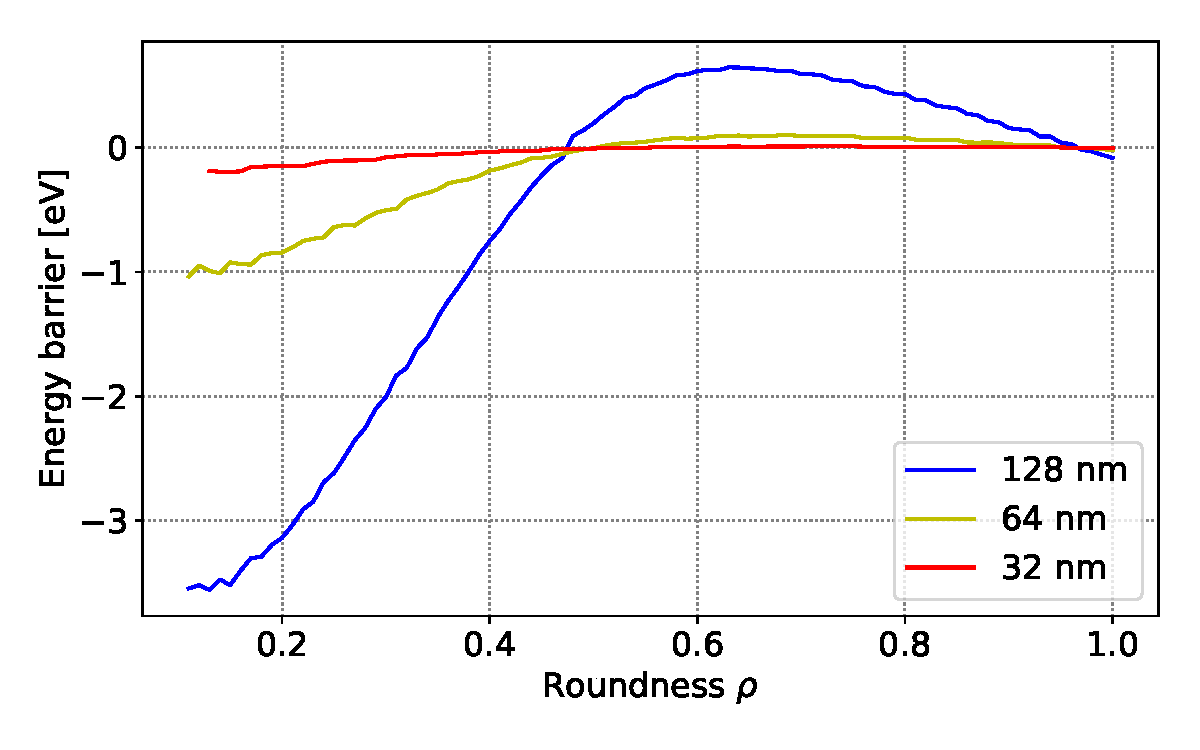
\includegraphics[width=0.9\columnwidth]{Figures/biaxial_island/Barrier/Plus_32,64,128_0.1-1_aPi128_B0.01_cell1nm.pdf}
    \caption{Energy barrier as a function of roundness $\rho$, for different total sizes $L$ as listed in the legend. Cell size \SI{1}{\nano\metre}. A positive value indicates that $E(\Theta=\pi/4) > E(\Theta=0)$, i.e. the hard axes are diagonal, while for a negative value the opposite is true.}
    \label{fig:barrier-cell_size}
\end{figure}
\begin{figure}
     \centering
     \begin{subfigure}[b]{0.2\textwidth}
         \centering
         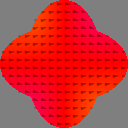
\includegraphics[width=\textwidth]{Figures/biaxial_island/BarrierMagnetization/mPlus_roundness0.60_a0.00.png}
        %  \caption*{Stable}
         \label{fig:barrier-magnetization-60x100_ortho}
     \end{subfigure}
     \hskip2em
     \begin{subfigure}[b]{0.2\textwidth}
         \centering
         
\includegraphics[width=\textwidth]{Figures/biaxial_island/BarrierMagnetization/mPlus_roundness0.60_a0.79.png}
        %  \caption*{Unstable}
         \label{fig:barrier-magnetization-60x100_diag}
     \end{subfigure}
     \vskip0em
    %  \vskip1em
     \begin{subfigure}[b]{0.2\textwidth}
         \centering
         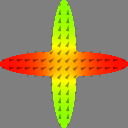
\includegraphics[width=\textwidth]{Figures/biaxial_island/BarrierMagnetization/mPlus_roundness0.20_a0.79.png}
         \caption*{$\uparrow$\\Stable}
         \label{fig:barrier-magnetization-20x100_diag}
     \end{subfigure}
     \hskip2em
     \begin{subfigure}[b]{0.2\textwidth}
         \centering
         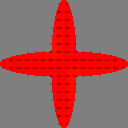
\includegraphics[width=\textwidth]{Figures/biaxial_island/BarrierMagnetization/mPlus_roundness0.20_a0.00.png}
         \caption*{$\uparrow$\\Unstable}
         \label{fig:barrier-magnetization-20x100_ortho}
     \end{subfigure}
    \caption{Relaxed magnetization for two different geometries with $L=\SI{100}{\nano\metre}$. The color hue represents the in-plane magnetization angle. \textbf{Top row:} roundness $\rho=0.6$. \textbf{Bottom row:} $\rho=0.2$. \textbf{Left column:} stable magnetization pattern. \textbf{Right column:} Unstable magnetization pattern.}
    \label{fig:barrier-magnetization}
\end{figure}
The geometry is the most important factor determining the energy barrier. Shown in \cref{fig:barrier-cell_size} is the dependence of the energy barrier on the roundness $\rho$, for different total sizes $L$. A positive value in this figure indicates that $E(\Theta=\pi/4) > E(\Theta=0)$, while for a negative value the opposite is true. This means that the first-order energy barrier is responsible for the sign in the plot, while it is the full energy barrier that is plotted. \par
The figure clearly shows that the energy barrier depends on the total size $L$. When halving $L$, the energy barrier becomes approximately 4 times smaller. As the thickness of the island is constant throughout these simulations, this indicates that the energy barrier is proportional to the volume of the island, as expected from theory. \par
The behavior as a function of the roundness $\rho$ is most clear by only looking at the blue curve of this figure, i.e. for $L=\SI{128}{\nano\metre}$. Interesting is that the sign of the energy barrier depends on $\rho$. A positive value corresponds to the long axes of the ellipses being the easy axes, while a negative value indicates that an average diagonal magnetization at \SI{45}{\degree} is favored. This can be understood by looking at the detailed magnetization pattern corresponding to $\widetilde{\Theta} = \SI{0}{\degree}$ and \SI{45}{\degree} in both regimes, as shown in \cref{fig:barrier-magnetization}. In general, the magnetization prefers a horizontal or vertical alignment, as these are the longest directions in the geometries. However, as the `lobes' get thinner for smaller $\rho$, it is no longer energetically favorable for the whole island to be magnetized uniformly, as this would not be along the long direction of at least two of the lobes. Instead, for islands with low $\rho$, a domain wall is created in the center, and the magnetization is rather uniform in each of the two ellipses separately. The sum of two such orthogonal magnetizations is on average diagonal, hence explaining the global behavior of the easy axes if one only observes the average magnetization angle $\widetilde{\Theta}$.
Interesting is the observation that there exists a $\rho \neq 1$ where the energy barrier switches sign, meaning that the easy and hard axes swap. Due to the higher order energy barrier as discussed previously, there will still exist a nonzero energy barrier for switching between two global minima spaced \SI{90}{\degree} apart. This can be seen in the figure as the sudden small but sharp drop around $\rho = 0.48$, where the function switches sign.

The energy barrier goes to zero for $\rho \rightarrow 1$, as one would expect for a perfectly round geometry. However, due to numerical error, the barrier is not calculated as exactly zero, which will be covered in the next section.

\subsubsection{Numerical error: influence of cell size on the energy barrier}
When performing more resource-intensive simulations, it is advantageous to use as large a cell size as possible in order to minimize the total amount of cells in the simulation. Increasing the size of the cells does, however, also increase the numerical error originating from the discretization of the grid. The size of this numerical error was examined by determining the energy barrier for different shapes (varying roundness and overall size) and for different cell sizes, viz. \SI{4}{\nano\metre}, \SI{2}{\nano\metre} and \SI{1}{\nano\metre}. The results of this calculation are shown in \cref{fig:barrier-cell_size-100nm}. \par
\begin{figure}
    \centering
    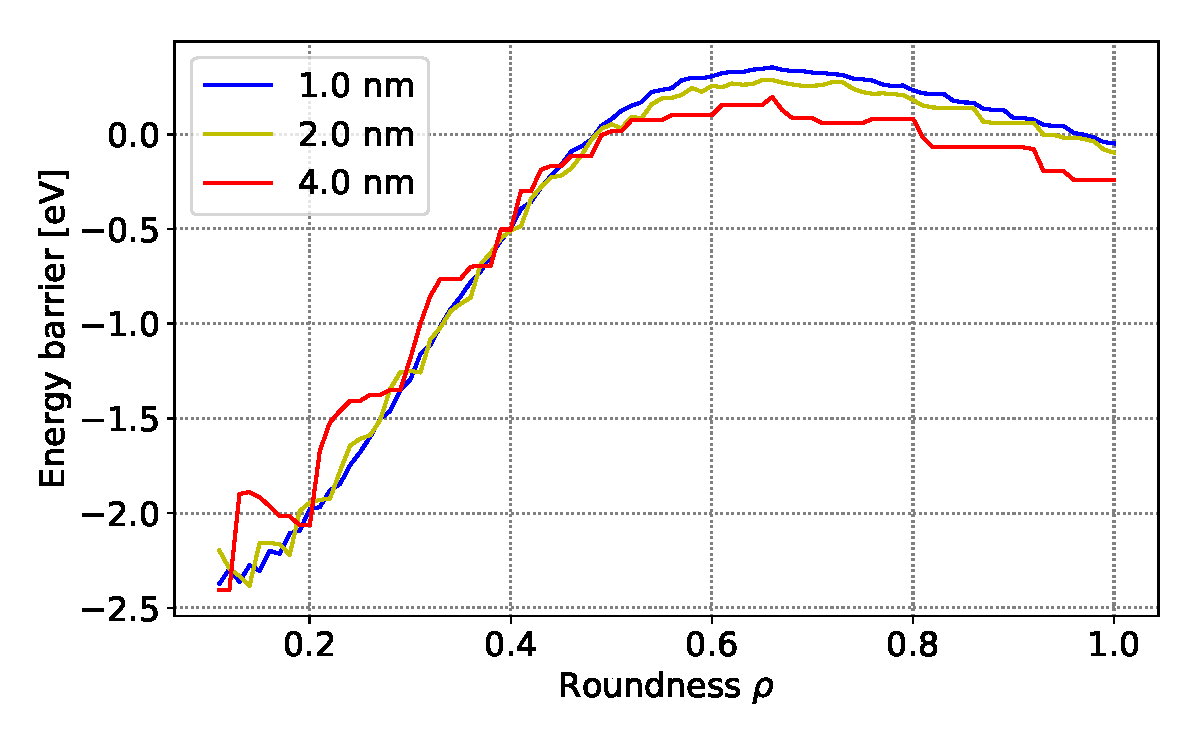
\includegraphics[width=0.9\columnwidth]{Figures/biaxial_island/Barrier/Plus_100_0.1-1_aPi128_B0.01_cell1,2,4nm.pdf}
    \caption{Energy barrier as a function of roundness $\rho$, for different cell sizes as listed in the legend. Long ellipse axis $L=\SI{100}{\nano\metre}$. A positive value indicates that $E(\Theta=\pi/4) > E(\Theta=0)$, i.e. the hard axes are diagonal, while for a negative value the opposite is true.}
    \label{fig:barrier-cell_size-100nm}
\end{figure}
The figure obtained with cells of \SI{1}{\nano\metre} is the smoothest, so it is justified that this size was used in the previous paragraphs. For \SI{2}{\nano\metre} cells, the curve becomes rougher, but the overall shape remains very similar to that of \SI{1}{\nano\metre} cells. Cells of \SI{4}{\nano\metre}, however, yield a very rough and almost stair-like energy landscape, which clearly indicates that \SI{4}{\nano\metre} cells are too large to get a physically accurate solution. \par
The global behavior as function of cell size, is that larger cells result in a lower value of the energy barrier. For nearly round geometries ($\rho \rightarrow 1$), the energy barrier becomes very large for a cell size of \SI{4}{\nano\metre} (\SI{240.7}{\milli\electronvolt}). In reality, a round geometry should of course not have a preferential direction. Because of the Cartesian simulation grid, however, a preferential orientation is created in the simulation. It was mentioned previously that the magnetization prefers to align itself along the longest direction of a given geometry. For a square, this is along the diagonals. When using the largest cells, the geometry most clearly consists of a bunch of squares, so the magnetization will be more inclined to align diagonally. When the hard axes are diagonal and the true physical energy barrier is large enough, or when the cells are small enough, the numerical error is not `strong' enough to swap the easy and hard axes. For small energy barriers and large cells, however, the effect is clearly noticeable, as is here the case for $\rho \rightarrow 1$. As the quantity plotted in \cref{fig:barrier-cell_size-100nm} is positive when the easy axes are horizontal and vertical, and negative when they are diagonal, the effect of the Cartesian grid is for the lines in the figure to drop down. \par
From the inset in the figure, which enlarges the region around $\rho=0.49$, it is observed that the energy barrier gets much closer to zero for the \SI{4}{\nano\metre} cells than it does for the smaller cells. As previously discussed, around $\rho=0.49$ the first-order energy barrier is approximately zero, and it are rather the higher-order terms which most significantly contribute to the total energy barrier. Thus, one can conclude that the higher-order energy barriers become smaller for larger cells. Because smaller cells more closely correspond to reality, it can finally be concluded that the higher-order energy barriers are definitely real, not just some numerical artefact. \par
Everything taken into account, it seems that the optimal compromise between simulation speed and accuracy, is a \SI{2}{\nano\metre} cell size. However, if one is solely interested in the physics corresponding to a specific value of the energy barrier, while making abstraction of other aspects like the geometry, any cell size can be used as long as the corresponding energy barrier for that discretization is known.

\subsubsection{Energy landscape in presence of an external magnetic field}
The sole purpose of the `virtual' external field $\vb{B_{ext,v}}$ used in the previous paragraphs was to make sure the magnetization remains at the energy maximum, in order to determine the value of this maximum. Of course, it is also possible to put the biaxial island in a real external field, simply denoted as $\vb{B_{ext}}$. This will make the Zeeman energy term of \cref{eq:Energy_Term_Zeeman} nonzero, hence adding a cosine function to the energy landscape. In order to visualize the energy landscape, the virtual external field is still necessary to stabilize the magnetization in the desired direction, away from the global minimum. This can be done in \mumax{} by using a custom field for the virtual external field and using the normal external field functionality for the real external field, hence decoupling the calculation of their energies and allowing the virtual field to be ignored afterwards when calculating the internal energy. As an example, the energy landscape for a situation where the external field was applied at $\chi=3\pi/8$ is shown in \cref{fig:barrierLandscape_extField}, where the additional cosine is clearly visible.
\begin{figure}[b!]
    \centering
    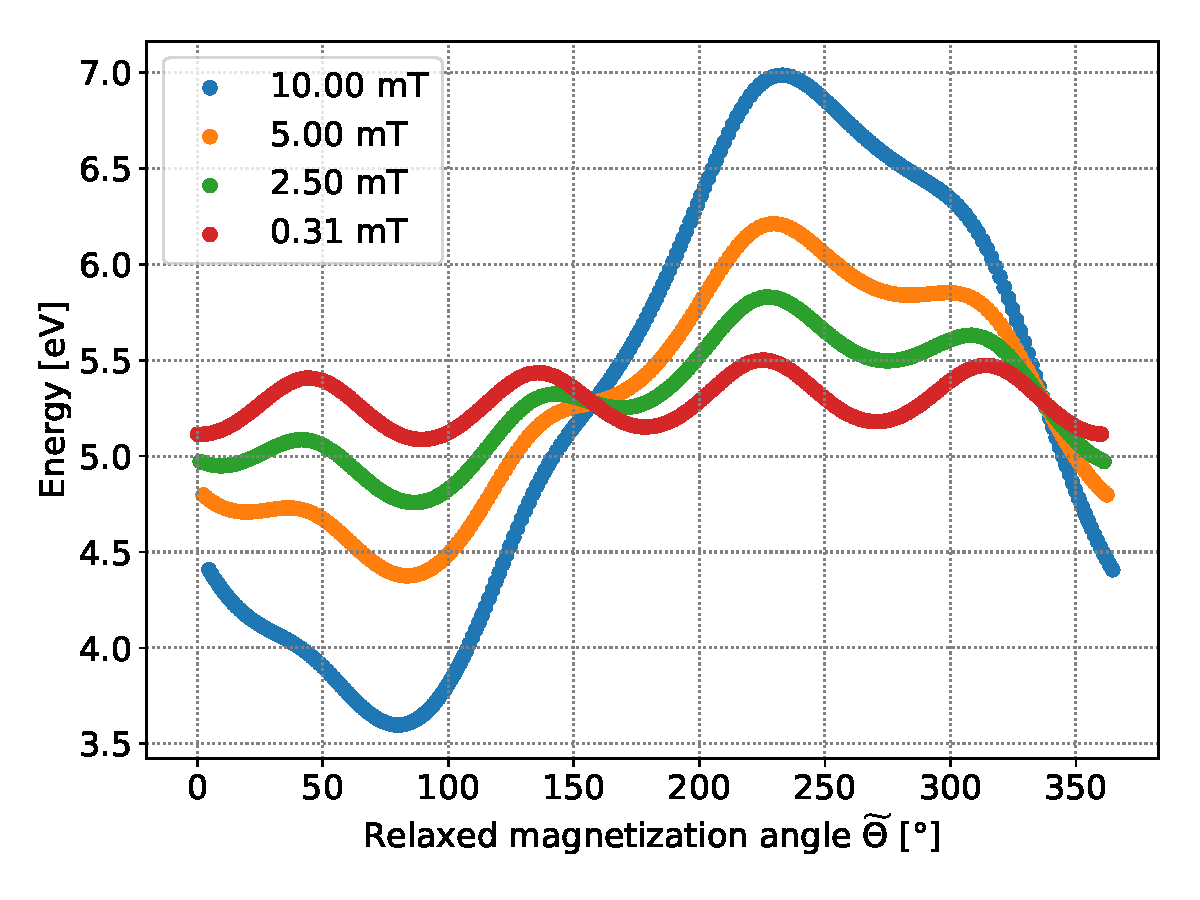
\includegraphics[width=0.9\columnwidth]{Figures/biaxial_island/BarrierLandscape/Ext_K0.1Ms2_Bext1e-2-1e-4_a3Pi8.pdf}
    \caption{Energy landscape as function of magnetization angle after relaxation, for different external field magnitudes $\abs{\vb{B_{ext}}}$ as listed in the legend, with the external field applied at an angle $\chi=3\pi/8$. The island geometry is $(\rho,L)=(0.65,\SI{100}{\nano\metre})$.}
    \label{fig:barrierLandscape_extField}
\end{figure}

\FloatBarrier
\subsection{Thermal switching}
Real nanomagnets exist at nonzero temperatures. These thermal fluctuations cause the magnetization of every atom to feel an additional random torque. When these fluctuations randomly add up to a sufficiently large torque, the magnetization can overcome the energy barrier and switch between two stable states. One of the main subjects of interest is the thermal switching frequency that accompanies a certain energy barrier.

\subsubsection{Theory}
Thermal switching is a random process, and can be modeled as being driven by a jump-noise process~\cite{MagDynamics_JumpNoise}, such that the time between two switches is given by the relationship
\begin{equation}
    t_i = -\frac{1}{f_0} \exp(\frac{E_{barrier}}{k_B T}) \ln(1-P_i) \mathrm{,}
    \label{eq:Switching_time}
\end{equation}
valid in the regime where $E_{barrier} \gg k_B T$.~\cite{RandomSwitch_MonteCarlo} Here, $P_i$ is a uniformly random number between 0 and 1. The average value of $-\ln(1-P_i)$ is then $\ln(4)$, which reduces \cref{eq:Switching_time} to
\begin{equation}
    t_i = \frac{\ln(4)}{f_0} \exp(\frac{E_{barrier}}{k_B T})  \mathrm{.}
    \label{eq:Switching_time_average}
\end{equation}
Conversely, if one needs to achieve a specific switching time $t_i$, the required energy barrier is given by
\begin{equation}
    E_{barrier} = k_B T \ln(\frac{f_0 t_i}{\ln(4)}) \mathrm{.}
\end{equation}
The main unknown in all previous equations is the attempt frequency $f_0$. As this parameter is crucial to achieve a correct estimate for the switching time, it will be determined both theoretically and through numerical simulations with the biaxial geometry. \par
A theoretical formula for $f_0$ (in \si{\radian\per\second}) in the case of uniaxial anisotropy~\cite{MuMax3, LEL-17b, f0_mumax3_reference} is given by
\begin{equation}
    f_0 = \gamma \frac{\alpha}{1+\alpha^2} \sqrt{\frac{4 K_{u1}^3 V}{\pi M_{sat}^2 k_B T}} \mathrm{,}
    \label{eq:f0_theoretical_uniaxial}
\end{equation}
with $\gamma$ the previously encountered gyromagnetic ratio equal to \SI{1.7595e11}{\radian\per\tesla\per\second}, $\alpha$ the dimensionless damping constant, $V$ the volume of the nanomagnet, and $K_{u1}$ and $M_{sat}$ the uniaxial anisotropy constant and saturation magnetization as defined in the Physics section. The anisotropy constant in general is simply the energy barrier corresponding to said anisotropy, divided by the volume of the particle. Hence, \cref{eq:f0_theoretical_uniaxial} can be adapted to a general anisotropic situation by substituting $K_{u1} \rightarrow E_{barrier}/V$, yielding
\begin{equation}
    f_0 = \gamma \frac{\alpha}{1+\alpha^2} \frac{2}{M_{sat} V} \sqrt{\frac{E_{barrier}^3}{\pi k_B T}} \mathrm{.}
    \label{eq:f0_theoretical_general}
\end{equation}
An alternative formula is found in \cite{f0_alternative_Jonathan}, which after simplification in the absence of an external field simply boils down to twice the value obtained from \cref{eq:f0_theoretical_general}, and thus yields the same order of magnitude. \par
Let us now estimate $f_0$ theoretically using \cref{eq:f0_theoretical_general} at \SI{300}{\kelvin} for a \SI{5}{\nano\metre} thick biaxial island with $L=\SI{100}{\nano\metre}$ made of Permalloy, a material for which $M_{sat}=\SI{8e5}{\ampere\per\metre}$.~\cite{MuMax3} The roundness is chosen such that $E_{barrier}=\SI{154.7}{\milli\electronvolt}$, as this is one of the barriers that will be used in the simulations later. Since the formulae for $f_0$ merely estimate its order of magnitude, the volume $V$ must not precisely be known and can hence be approximated by the volume of a circular ($\rho=1$) geometry, i.e. $V\approx\SI{4e-23}{\metre\cubed}$. The damping constant is taken as $\alpha=0.01$. \par
This yields a theoretical estimate of $f_0 = \SI{6e6}{\per\second}$. We will compare this to the experimental values obtained through simulations with \mumax{} in the next section.

\subsubsection{Simulations}
Given the total simulation time $\tau$ and the number of switches $N$ during this time interval, an estimate for $f_0$ can be derived from \cref{eq:Switching_time} as
\begin{equation}
    f_0 = \frac{N \ln(4)}{\tau} \exp(\frac{E_{barrier}}{k_B T}) \mathrm{.}
    \label{eq:f0_experimental}
\end{equation}
There exists some ambiguity as to how one can count the amount of switches during a time interval. The method applied here counts every monotone rotation of the magnetization over more than \SI{90}{\degree} in either direction as a switch. Hence, not every crossing of an energy maximum is counted as a separate switch; when the magnetization rotates through multiple energy maxima in quick succession, such switches larger than \SI{90}{\degree} are counted as one single switch. As soon as the magnetization starts turning in the opposite direction, any subsequent \SI{90}{\degree} turn or larger is counted as another switch. \par 
\ctable[
    cap = Switching Rates,
    caption = {Switching rates and corresponding $f_0$ values for different energy barriers (determined by the roundness $\rho$ and grid discretization), temperatures and values of the damping constant. $L=\SI{100}{\nano\metre}$ and $M_{sat}=\SI{8e5}{\ampere\per\metre}$ for all entries.},
    label = {tab:Switching_f0},
    pos = ht,
    %sideways
    ]{
    c|c||c|c|c|c|c||c
    }{
    \tnote[a]{This energy barrier is comparable to the thermal energy $k_B T$. Hence, the switching rate ($\approx \SI{2}{\nano\second}$) is on the same timescale as the LLG dynamics, which causes the estimate for $f_0$ using \cref{eq:f0_theoretical_general} to be inaccurate.}
    }{
        $\rho$ & Grid [nm] & Barrier [meV] & T [K] & $\alpha$ & $\tau$ [ns] & $N$ & $f_0$ \\
        \hline
        0.49 & 2 & 27.8\tmark[a] & 300 & 0.01 & 100 & 37 & \SI{1.50e9}{} \\
        \hline
        0.65 & 4 & 154.7 & 273 & 0.01 & 1000 & 13 & \SI{1.29e10}{} \\
        0.65 & 4 & 154.7 & 300 & 0.1 & 1000 & 12 & \SI{6.61e9}{} \\
        0.65 & 4 & 154.7 & 300 & 0.01 & 1000 & 11 & \SI{6.05e9}{} \\
        0.65 & 4 & 154.7 & 350 & 0.01 & 1000 & 41 & \SI{9.60e9}{} \\
        0.65 & 2 & 286.2 & 350 & 0.01 & 500 & 0 & 0 \\
        0.65 & 3.125 & 207.9 & 350 & 0.01 & 1000 & 9 & \SI{1.23e10}{} \\
        \hline
        1 & 4 & 240.7 & 300 & 0.01 & 1000 & 0 & 0 \\
        1 & 4 & 240.7 & 350 & 0.01 & 1000 & 5 & \SI{2.03e10}{} 
    }
Several simulations were carried out for $\tau$ up to \SI{1}{\micro\second}, where the temperature $T$, the energy barrier and damping constant $\alpha$ were varied. Examples of such simulations are shown in \cref{fig:switching-alpha,fig:switching-temp,fig:switching-49x100-300}, and a summary of all conducted simulations is given in \cref{tab:Switching_f0}. For each simulation, a theoretical value for $f_0$ was estimated using \cref{eq:f0_experimental} as listed in the last column of the table. 
Nearly all simulations for which the energy barrier is significantly higher than the thermal energy yield a value around $f_0=\SI{e10}{\per\second}$, apart from some outliers which did not switch within $\tau$. Unfortunately, this estimate is three orders of magnitude larger than the theoretical estimate determined in the previous section. This indicates that the theoretical \cref{eq:f0_theoretical_general} is not applicable. The reason for this is unclear; perhaps because the magnetization is not perfectly uniform in the simulation, which is one of the assumptions underlying the theoretical formula. \par
The value obtained through the simulations is, however, on the same order of magnitude as the intrinsic resonance frequency of the small sinus of the energy minimum.
Apart from the quantitative measure for $f_0$, some qualitative aspects of changing the parameters will now be addressed.

\paragraph{Effect of damping constant $\alpha$}
\begin{figure}
     \centering
     \begin{subfigure}[b]{0.8\textwidth}
         \centering
         \includegraphics[width=\textwidth]{Figures/biaxial_island/Switching/65x100_300K_alpha0.1_1µs_4nm_INSET.pdf}
         \caption{$\alpha=0.1$}
         \label{fig:switching-alpha-0.1}
     \end{subfigure}
     \hfill
     \begin{subfigure}[b]{0.8\textwidth}
         \centering
         \includegraphics[width=\textwidth]{Figures/biaxial_island/Switching/65x100_300K_alpha0.01_1µs_4nm_INSET.pdf}
         \caption{$\alpha = 0.01$}
         \label{fig:switching-alpha-0.01}
     \end{subfigure}
        \caption{Switching for two different values of the damping constant $\alpha$, with a grid discritization of \SI{4}{\nano\metre} at \SI{300}{\kelvin}, for $(\rho, L) = (0.65, \SI{100}{\nano\metre})$.}
        \label{fig:switching-alpha}
\end{figure}
The effect of changing the damping constant $\alpha$ is shown in \cref{fig:switching-alpha}. There is a clear qualitative difference between $\alpha=0.1$ (\cref{fig:switching-alpha-0.1}) and $\alpha=0.01$ (\cref{fig:switching-alpha-0.01}). For higher $\alpha$, only single switches occur, i.e. \SI{90}{\degree} between adjacent energy minima. For lower damping, switching may occur over more than \SI{90}{\degree}; as an example, there are three switches over \SI{180}{\degree} visible in \cref{fig:switching-alpha-0.01}. This is understandable since the magnetization can be seen as a rotating body as described earlier in the Physics section. Hence, less damping implies that the magnetization will more easily retain its angular velocity after overcoming the first energy maximum, and can thus overcome multiple energy barriers in quick succession. \par
From \cref{eq:H_therm}, which gives an expression for the thermal field, it is clear that the magnitude of this thermal field is proportional to the square root of the damping constant. The effect of this is noticeable in the inset figures of \cref{fig:switching-alpha}. For $\alpha=0.01$, the magnetization rotates in a smooth manner, simply oscillating quasi-harmonically in one of the four energy valleys. Because the coupling to the thermal field is weak, the thermal field only introduces randomness in the amplitude of this oscillation, and does not significantly distort the sinusoidal pattern itself. For a higher $\alpha=0.1$, the rotation exhibits more jagged behavior, on the one hand due to the higher damping, on the other hand due to the larger coupling with the thermal field. \par
Quantitatively, the effect of $\alpha$ on $f_0$ can be examined by comparing rows 3 and 4 of \cref{tab:Switching_f0}. There does not seem to be a significant dependence on the damping constant $\alpha$, contrary to the inverse proportionality predicted by the theory of \cref{eq:f0_theoretical_general}, further indicating that the theoretical formula does not apply. Note, however, that the estimate $f_0\approx\SI{e10}{\per\second}$ is quite close to the frequency of the intrinsic oscillation visible in the inset figures (\cref{fig:switching-alpha-0.01}), which has a period of \SI{0.5}{\nano\second}. It is logical that these two are related, as one can see this oscillation as an `attempt' to leave the energy minimum once every half-period.

\FloatBarrier
\paragraph{Effect of temperature and energy barrier}
It is expected that $f_0$ exhibits an exponential dependency on the ratio between energy barrier and temperature. To confirm this, simulations spanning \SI{1}{\micro\second} were carried out for two different temperatures and two different energy barriers. The different energy barriers correspond to $\rho=0.65$ (\SI{154.7}{\milli\electronvolt}) and $\rho=1$ (\SI{240.7}{\milli\electronvolt}) geometries at a cell size of \SI{4}{\nano\metre}. Such a large cell size was chosen because these simulations take a long time to calculate, and we are only interested in the behavior accompanying a certain energy barrier, while making abstraction of all other aspects. Note that these two geometries have opposite easy and hard axes. This is clearly visible in the figures, as the \SI{154.7}{\milli\electronvolt} case is stable around $n\SI{90}{\degree}$, $n \in \mathbb{Z}$, while \SI{240.7}{\milli\electronvolt} is stable around $\SI{45}{\degree} + n\SI{90}{\degree}$. The exponential dependence on the temperature is qualitatively clear from the difference between \cref{fig:switching-temp-300-65x100,fig:switching-temp-350-65x100}, where the latter switches significantly more for only a \SI{16}{\percent} increase in temperature. The exponential dependence on the energy barrier can be seen in the difference between \cref{fig:switching-temp-300-65x100,fig:switching-temp-300-100x100}, where the latter has not a single switch due to the \SI{55}{\percent} higher energy barrier. The numerical value for $f_0$ is also for these simulations close to \SI{e10}{\per\second}, as listed in \cref{tab:Switching_f0}.
\begin{figure}
     \centering
     \begin{subfigure}[b]{0.49\textwidth}
         \centering
         \includegraphics[width=\textwidth]{Figures/biaxial_island/Switching/65x100_300K_alpha0.01_1µs_4nm.pdf}
         \caption{\SI{300}{\kelvin}, \SI{154.7}{\milli\electronvolt}}
         \label{fig:switching-temp-300-65x100}
     \end{subfigure}
     \hfill
     \begin{subfigure}[b]{0.49\textwidth}
         \centering
         \includegraphics[width=\textwidth]{Figures/biaxial_island/Switching/65x100_350K_alpha0.01_1µs_4nm.pdf}
         \caption{\SI{350}{\kelvin}, \SI{154.7}{\milli\electronvolt}}
         \label{fig:switching-temp-350-65x100}
     \end{subfigure}
     \begin{subfigure}[b]{0.49\textwidth}
         \centering
         \includegraphics[width=\textwidth]{Figures/biaxial_island/Switching/100x100_300K_alpha0.01_1µs_4nm.pdf}
         \caption{\SI{300}{\kelvin}, \SI{240.7}{\milli\electronvolt}}
         \label{fig:switching-temp-300-100x100}
     \end{subfigure}
     \hfill
     \begin{subfigure}[b]{0.49\textwidth}
         \centering
         \includegraphics[width=\textwidth]{Figures/biaxial_island/Switching/100x100_350K_alpha0.01_1µs_4nm.pdf}
         \caption{\SI{350}{\kelvin}, \SI{240.7}{\milli\electronvolt}}
         \label{fig:switching-temp-350-100x100}
     \end{subfigure}
    \caption{Switching for two different energy barriers and two temperatures, with a grid discritization of \SI{4}{\nano\metre} and $\alpha = 0.01$. The energy barrier of \SI{154.7}{\milli\electronvolt} corresponds to a geometry with $\rho=0.65$, and \SI{240.7}{\milli\electronvolt} to $\rho=1$.}
    \label{fig:switching-temp}
\end{figure}

\paragraph{Limit of low barrier}
\begin{figure}
    \centering
    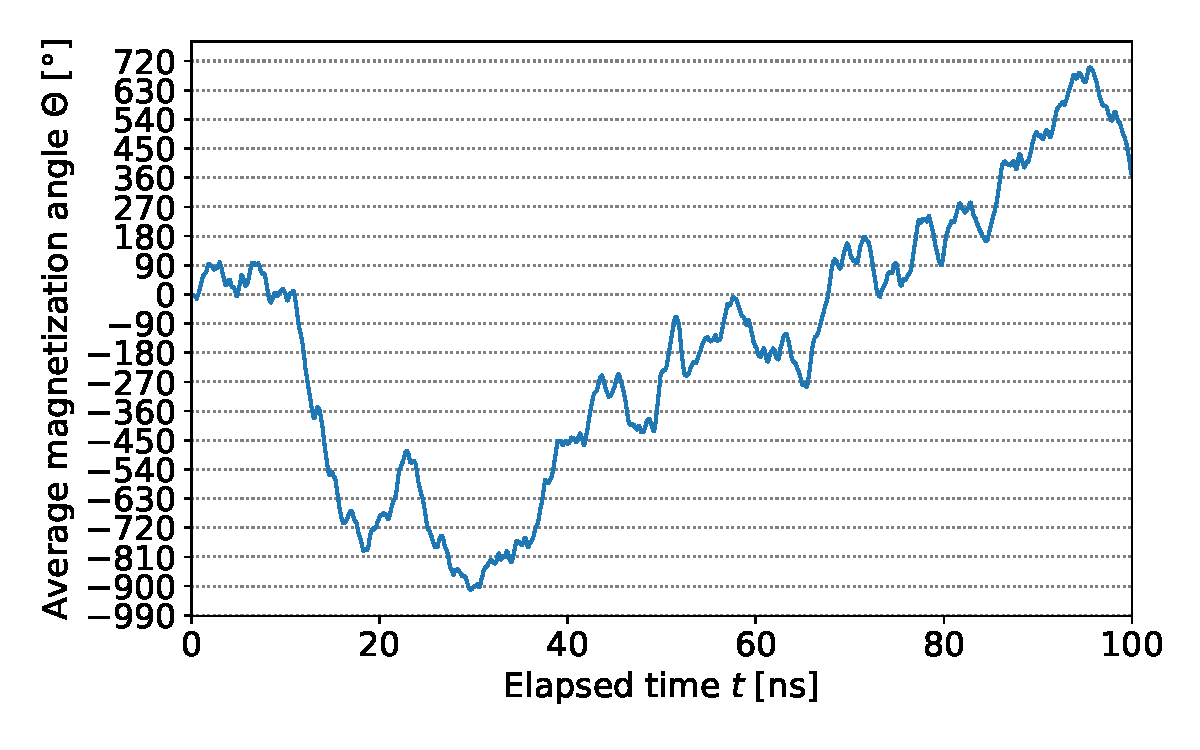
\includegraphics[width=0.8\columnwidth]{Figures/biaxial_island/Switching/49x100_300K_alpha0.01_100ns_2nm.pdf}
    \caption{Switching for an energy barrier of \SI{27.8}{\milli\electronvolt}, corresponding to $\rho=0.49$ for a grid discretization of \SI{2}{\nano\metre}. Temperature \SI{300}{\kelvin} and $\alpha = 0.01$.}
    \label{fig:switching-49x100-300}
\end{figure}
In the limit where the energy barrier is comparable to the thermal energy $k_B T$, the exponential law from \cref{eq:f0_experimental} no longer holds, because that law is based on the assumption that the magnetization angle distribution is sufficiently concentrated near an energy minimum.~\cite{ThermFluc_SingleDomain}
For such a low barrier, the switching rate is on the same timescale as the LLG dynamics, such that besides the energy barrier, now also these dynamics play a major role. An example of a \SI{100}{\nano\second} simulation for an energy barrier of \SI{27.8}{\milli\electronvolt} is shown in \cref{fig:switching-49x100-300}. As one would expect, the magnetization does not get stuck in any of the energy minima because they are too shallow. The switching frequency for such a low barrier comes close to that of the intrinsic sinusoidal pattern visible in the inset of \cref{fig:switching-alpha-0.01}.


\clearpage
\section{Interaction between two islands}
The interaction between two islands can be seen as the contribution of three components: the shape anisotropy of the first island, the shape anisotropy of the second island, and the interaction energy between them. The anisotropy of an island has already been examined in \cref{par:Biaxial_EnergyBarrier}, and depends on its average magnetization angle $\Theta$, total size $L$, and roundness $\rho$. It is expected that the interaction energy between two islands will depend on the distance $d$ between centers of the two islands, the average magnetization angle $\Theta_i$ of each island, their total size $L$, and perhaps to a lesser degree also the roundness $\rho$ and orientation $\Phi_i$ of each island with respect to their common axis. \par
Care needs to be taken that each island is placed on the grid in the correct manner, i.e. such that the numerical energy barrier is known correctly. To keep things simple, the two islands will be kept identical as much as possible. This means that islands with the same rotation $\Phi$ must be placed on identical positions with respect to the cells of the numerical grid.

\subsection{Interaction energy as function of magnetization angle}
\label{par:TwoIslands_InteractionAngle}
\begin{figure}
    \centering
    \begin{subfigure}[c]{4cm} % no problem: this appears blurry online but offline it is nice and sharp
         \centering
         
\includegraphics[width=\textwidth]{Figures/two_islands/Geometry/geom_r0.49_s100_d128_a0,0_cell4nm.png}
     \end{subfigure}
    \begin{subfigure}[c]{0.7\columnwidth}
         \centering
         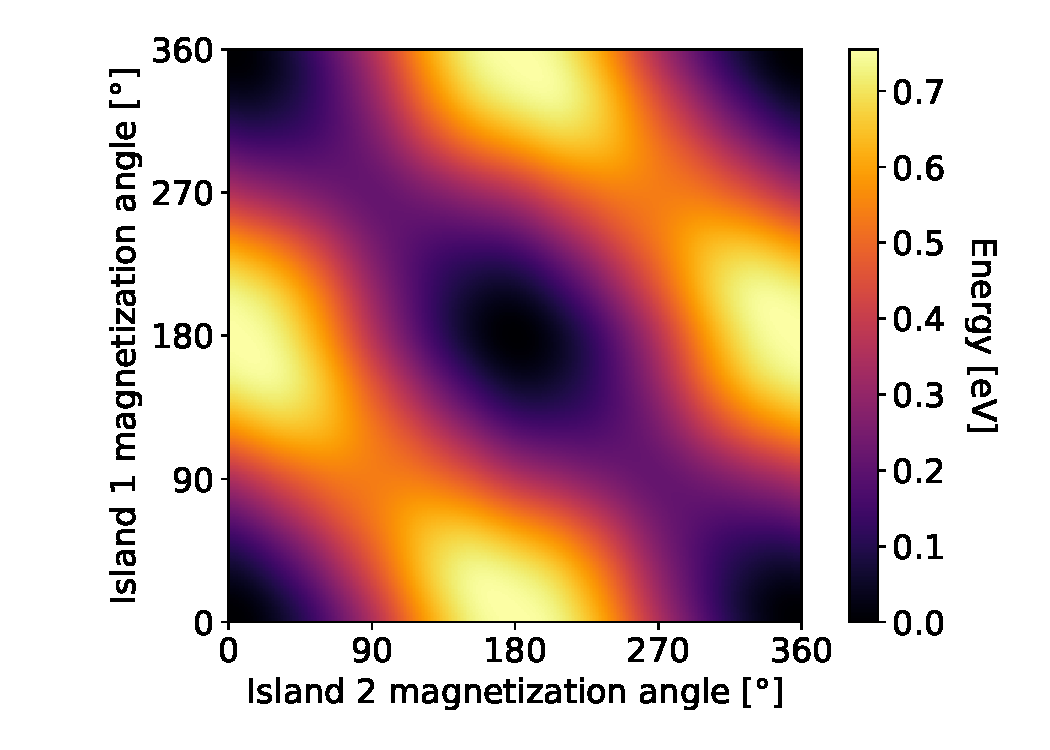
\includegraphics[width=\textwidth]{Figures/two_islands/EnergyLandscape/Int_a0Pi,0Pi_d128_r0.49,0.49_cell4nm.pdf}
     \end{subfigure}
    \caption{\textbf{Left:} geometry for two $(\rho, L)~=~(0.49, \SI{100}{\nano\metre})$ islands spaced \SI{128}{\nano\metre} apart, with \SI{4}{\nano\metre} grid. Corresponding $E_{barrier}=\SI{5.1}{\milli\electronvolt}$. \textbf{Right:} interaction energy as function of the magnetization angle of each island.}
    \label{fig:two-islands_interaction_(r0.49_L100)_a0and0}
\end{figure}
\begin{figure}
    \centering
    \begin{subfigure}[c]{4cm} % no problem: this appears blurry online but offline it is nice and sharp
         \centering
         
\includegraphics[width=\textwidth]{Figures/two_islands/Geometry/geom_r0.66_s100_d128_a0,0_cell1nm.png}
     \end{subfigure}
    \begin{subfigure}[c]{0.7\columnwidth}
         \centering
         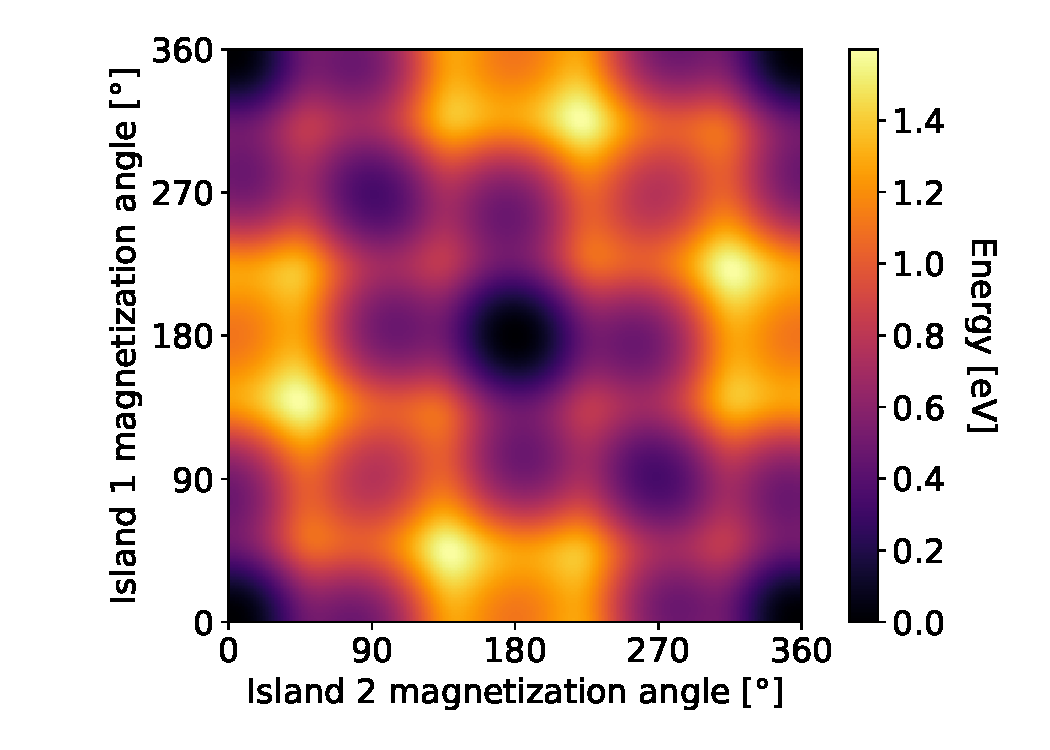
\includegraphics[width=\textwidth]{Figures/two_islands/EnergyLandscape/Int_a0Pi,0Pi_d128_r0.66,0.66_cell1nm.pdf}
     \end{subfigure}
    \caption{\textbf{Left:} geometry for two $(\rho, L)~=~(0.66, \SI{100}{\nano\metre})$ islands spaced \SI{128}{\nano\metre} apart, with \SI{1}{\nano\metre} grid. Corresponding $E_{barrier}=\SI{352.6}{\milli\electronvolt}$. \textbf{Right:} interaction energy as function of the magnetization angle of each island.}
    \label{fig:two-islands_interaction_(r0.66_L100)_a0and0}
\end{figure}
\begin{figure}
    \centering
    \begin{subfigure}[c]{4cm} % no problem: this appears blurry online but offline it is nice and sharp
         \centering
         
\includegraphics[width=\textwidth]{Figures/two_islands/Geometry/geom_r0.66_s100_d128_aPi4,Pi4_cell1nm.png}
     \end{subfigure}
    \begin{subfigure}[c]{0.7\columnwidth}
         \centering
         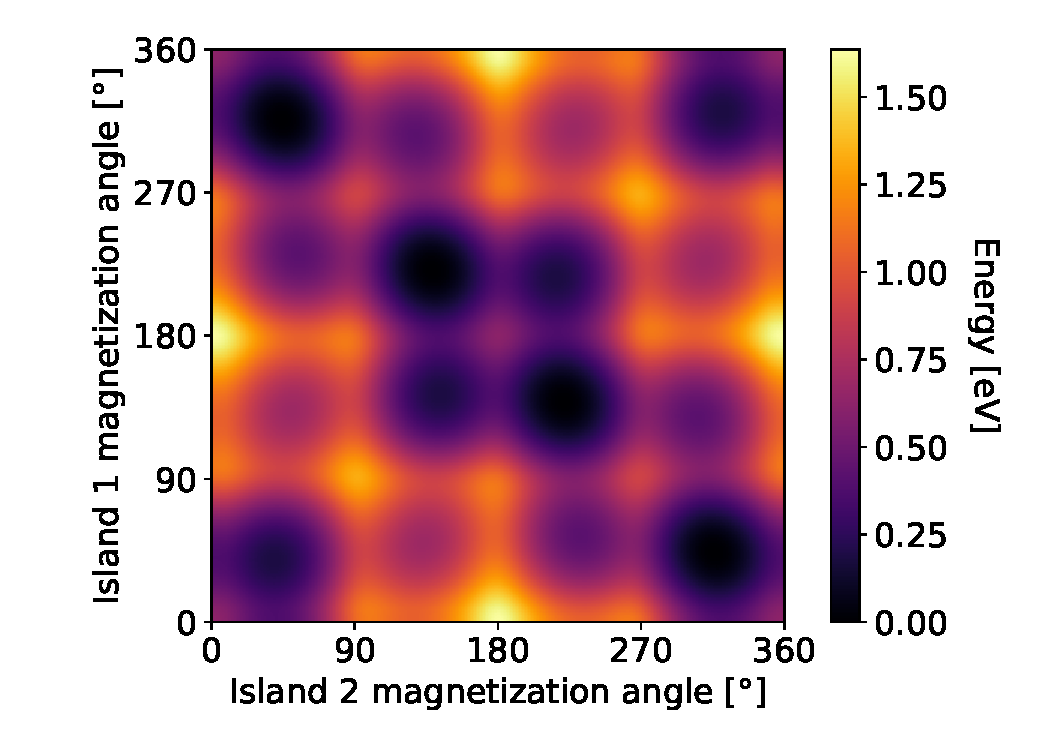
\includegraphics[width=\textwidth]{Figures/two_islands/EnergyLandscape/Int_aPi4,Pi4_d128_r0.66,0.66_cell1nm.pdf}
     \end{subfigure}
    \caption{\textbf{Left:} geometry for two $(\rho, L)~=~(0.66, \SI{100}{\nano\metre})$ islands spaced \SI{128}{\nano\metre} apart, both rotated over $\Phi=\pi/4$, with \SI{1}{\nano\metre} grid. Corresponding $E_{barrier}=\SI{419.3}{\milli\electronvolt}$. \textbf{Right:} interaction energy as function of the magnetization angle of each island.}
    \label{fig:two-islands_interaction_(r0.66_L100)_aPi4andPi4}
\end{figure}
\subsubsection{Without biaxial anisotropy}
In order to investigate the interaction energy, and the interaction energy only, the islands should be chosen such that their anisotropy is minimal. This can be achieved by choosing the roundness $\rho$ for which the energy barrier is closest to zero according to \cref{fig:barrier-cell_size-100nm}. For an island with size $L=\SI{100}{\nano\metre}$, the energy barrier is minimal for $\rho=0.49$. \par
Figure~\ref{fig:two-islands_interaction_(r0.49_L100)_a0and0} shows the energy landscape for two adjacent $(\rho, L)=(0.49, \SI{100}{\nano\metre})$ islands with their centers spaced $d=\SI{128}{\nano\metre}$ apart, as a function of their magnetization angles. There are 4 distinct equilibria in this figure, if one makes abstraction of global rotations and symmetries: $(\Theta_1, \Theta_2) = (0,0), (0, \pi), (\frac{\pi}{2}, \frac{\pi}{2})$ and $(\frac{\pi}{2}, -\frac{\pi}{2})$. The lowest energy configuration is that where both islands are magnetized in the same direction along their common axis, $(\Theta_1, \Theta_2) = (0,0)$. Conversely, the highest energy occurs for opposite magnetization along this common axis, $(\Theta_1, \Theta_2) = (0,\pi)$. The two other equilibria are saddle points, corresponding to two distinct situations where both islands are magnetized perpendicularly to their common axis. The one with lowest energy of these two has the two islands oppositely magnetized, $(\Theta_1, \Theta_2) = (\frac{\pi}{2}, -\frac{\pi}{2})$, while the case with parallel magnetizations $(\Theta_1, \Theta_2) = (\frac{\pi}{2}, \frac{\pi}{2})$ has higher energy. This discussion sounds familiar, because the figure simply gives a geometric representation of the behavior discussed at the start of \cref{par:Intro_nanomagnetic-islands} and \cref{fig:Intro_IslandEllipticPreferredDirection}, but now for two separate islands instead of exchange-coupled magnetic moments. The figure does, however, give us some new information, namely that the configuration with opposite magnetization perpendicular to the common axis has higher energy than for parallel magnetization along the common axis. On a similar note, the energy landscape teaches us that switching between energy minima preferably occurs by rotating the magnetization of the two islands in opposite directions.

\subsubsection{With biaxial anisotropy}
Figure~\ref{fig:two-islands_interaction_(r0.66_L100)_a0and0} shows the total energy of two interacting islands, but now with nonzero shape anisotropy. To make the contribution of this shape anisotropy to the energy landscape as clear as possible, a geometry with high barrier ($\rho=0.66$) and a small grid (\SI{1}{\nano\metre}) were chosen. As one would expect, this anisotropy simply superposes a sinusoidal pattern with period $\frac{pi}{2}$ in the figures, in both the vertical and horizontal directions, thus creating 16 local minima and maxima. Obviously, if one rotates one of these islands, its anisotropy axes will rotate as well, manifesting itself in the figure as a translation of this sinusoidal pattern. As compared to the case without anisotropy, one would expect the total height of the energy landscape to increase by double the energy barrier, i.e. \SI{705.2}{\milli\electronvolt}. However, the total height of the energy landscape has increased more than this, as can be seen from the colorbar on the right hand side of the figures. This can be explained by the fact that, for a $\rho=0.66$ geometry, the volume of the islands is larger than for a $\rho=0.49$ geometry. The increase in energy caused by this additional volume will be significantly higher the closer this additional volume is to the other island, due to the relationship discussed in \cref{par:TwoIslands_EnergyHeight}. This can be confirmed by performing a simulation at $\rho=0.81$ for \SI{4}{\nano\metre} cells, which is another geometry without anisotropy as shown in \cref{par:Biaxial_island}. This simulation yields an energy landscape height of \SI{1.37}{\electronvolt} for $\rho=0.81$, as compared to the \SI{0.74}{\electronvolt} for $\rho=0.49$, clearly showing that the additional volume close to the other island has a significant effect on the energy landscape height. \par
Figure~\ref{fig:two-islands_interaction_(r0.66_L100)_aPi4andPi4} shows the energy landscape of two interacting islands rotated over $\Phi=\pi/4$, yielding the geometry on the left of the figure. As evident from the caption, these rotated islands have a different numerical energy barrier compared to their non-rotated counterparts, due to the different orientation of the numerical grid with respect to the geometry of the islands. As was already suggested in the introduction, this geometry can be used as a balanced nanomagnetic logic chain due to its high degree of symmetry. In the energy landscape, there are clearly four identical global minima, along $\Theta_1 = -\Theta_2$. Suppose the leftmost island (island 1) is the input of this chain, then it is energetically favorable for the second island to have its magnetization be the input island's magnetization mirrored over the horizontal axis. This holds for all four stable orientations of the magnetization of the first island, and all these have equal ground state energy, thus confirming the geometry is balanced.

\subsection{Energy landscape height as function of distance between islands}
\label{par:TwoIslands_EnergyHeight}
\begin{figure}
    \centering
    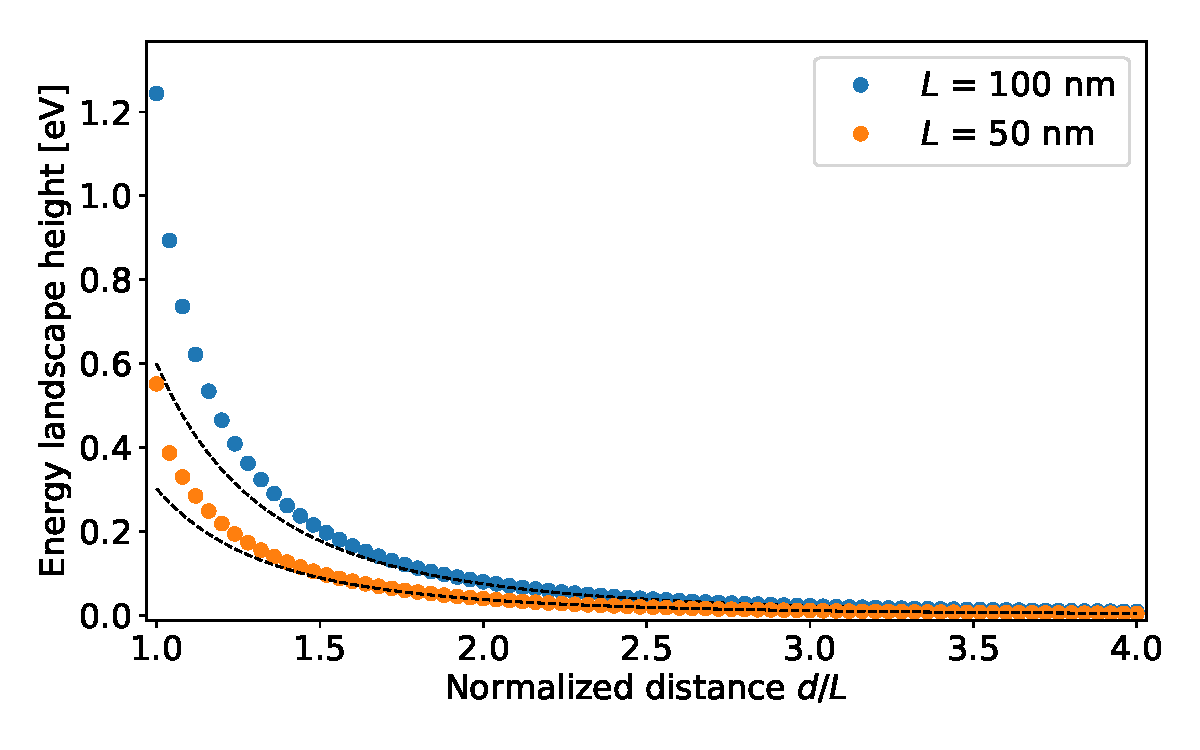
\includegraphics[width=0.8\columnwidth]{Figures/two_islands/EnergyBarrier/dist1-4L_r0.49_s100&50_4nm&2nm.pdf}
    \caption{Height of the interaction energy landscape for two different island sizes $L$ as listed in the legend, as a function of the normalized distance $d/L$ between the two islands. The dotted lines indicate an ideal $1/d^3$ relationship.}
    \label{fig:two-islands_barrier}
\end{figure}
When halving all dimensions of the simulation, like cell size, inter-island distance, and island size, the energy landscape height also halves, as evident from \cref{fig:two-islands_barrier}. In this figure, the height of the energy landscape is shown as a function of the distance between the two islands, and this for two identical but scaled geometries as listed in the legend. For two magnets at a large distance from each other, it is known~\cite{MagnetForceDistance} that the force $F \propto V^2 / d^4$, and since $F=\partial E/\partial x$ it follows that
\begin{equation}
    E \propto V^2 / d^3 \mathrm{.}
    \label{eq:two-islands_distance}
\end{equation}
This is exactly the behavior that is seen in the figure. When halving all dimensions, $V$ becomes 4 times smaller because the thickness of the islands is kept the same, and $d$ simply halves as well. The combination of these two in \cref{eq:two-islands_distance} then causes the energy $E$ to be halved, as is observed in the figure. \par
For both values of $L$, a $1/d^3$ fit is drawn as a dotted line, which coincides with the data at $d/L=4$ to ensure a correct energy scale for this fit. As the distance $d$ is measured between the centres of the islands, a normalized distance $d/L=1$ corresponds to two touching islands. For such small distances, the approximation of \cref{eq:two-islands_distance} is clearly no longer applicable, and the $1/d^3$ fit significantly deviates from the true relationship. Due to the exchange energy working at very small distances, the height of the energy landscape for $d/L=1$ is significantly higher than for all higher values of $d/L$.

\clearpage
\section{Half adder}
\label{par:halfadder}
A half adder is a logic gate which adds two binary input bits. In the case where these two input bits are 1 and 1, the output should thus be 2. Since the binary representation of 2 is `10', two output bits are required to represent the output, the first of which is referred to as `carry', the second as `sum'. Thus, a half adder takes two bits as input and yields two bits as output, the truth table of which is given in the left half of \cref{tab:HalfAdder}. For this reason, it could be advantageous to realize a half adder using biaxial nanomagnets, as a single biaxial island has 4 stable states and can thus represent exactly two bits of information. As such, a half adder realized with biaxial nanomagnets only has one input island and one output island. The truth table of a half adder, now in the quaternary numeral system inherent to biaxial nanomagnets, is shown in the right half of \cref{tab:HalfAdder}. The use of biaxial nanomagnets will require us to work with the quaternary version of the truth table from now on. In this quaternary system, the meaning of a half adder as being an `adder' is no longer as clear, though of course this meaning is still relevant as it can easily be recovered by returning to the binary counting system. \par
\ctable[
    cap = Half Adder,
    caption = {Truth table for a half adder, both in binary and quaternary numeral systems.},
    label = {tab:HalfAdder},
    pos = ht,
    mincapwidth = \columnwidth
    ]{
    %r|l||r|l
    c|c||c|c % paps vindt dit beter
    }{}{
        \multicolumn{2}{c||}{Binary} & \multicolumn{2}{c}{Quaternary} \\
        \hline
        Input & Output & Input & Output \\
        \hline
        00 & 00 & 0 & 0 \\
        01 & 01 & 1 & 1 \\
        10 & 01 & 2 & 1 \\
        11 & 10 & 3 & 2 \\
    }
\subsection{Nanomagnetic half adders}
\subsubsection{Quaternary convention}
When designing a logic gate using nanomagnets, one always has to define what the meaning is of each magnetization direction. For uniaxial nanomagnets, one needs to define whether `up' corresponds to a 0 or a 1, and vice versa for `down'. For biaxial nanomagnets, there are four directions which have to be assigned a number from 0 to 3. There are 24 possible ways to do this: for the first direction there are four numbers to choose from, for the second there are three, for the third only two, and for the fourth direction only one possible number remains. We will refer to such a choice as the `quaternary convention'. We will always list the quaternary convention in the form $(\SI{0}{\degree}, \SI{90}{\degree}, \SI{180}{\degree}, \SI{270}{\degree})$, assuming the geometry of a single island is that of \cref{fig:biaxial_island:geometryTypical}, with the angles defined in the usual anticlockwise mathematical manner with \SI{0}{\degree} corresponding to a magnetization to the right. A given geometry of nanomagnets, with given input and output islands, will only behave as a half adder for at most one quaternary convention. When choosing a different input or output island, the relevant quaternary convention may be different, or of course nonexistent if no half adder is possible for that particular choice of input and output islands. Thus, given a geometry of $N$ free nanomagnetic islands, i.e. whose magnetization direction is not fixed, there are $N$ possible choices for the input island, $N-1$ remaining choices for the output island, and for each combination of input and output there are 24 possible quaternary conventions to try. Only a select few, if any, of these $24N(N-1)$ possible combinations will correctly give the geometry the meaning of a half adder. Note that this assumes the same quaternary convention for the input and output, which is not explicitly necessary, but eliminates unnecessary problems that will occur if one were to use a different convention between the input and output. \par
A given geometry, for a certain choice of input and output island, is said to function as a half adder if there exists a quaternary convention for which the lowest energy state for each of the 4 possible input magnetization angles has the correct output magnetization angle. If this is the case, one can use the half adder for a forward calculation: when fixing the input, the lowest energy configuration will have the correct orientation of the output magnetization. Note that this is not sufficient for the gate to be usable for a reverse calculation; for this, a balanced geometry is necessary, meaning that all of these 4 ground states have equal energy, making them equally likely to occur. \par
Take as an example \cref{fig:HalfAdder_000006_configurations_In1_0213}, where the blue island to the left represents the input, and the red island to the right represents the output. The geometry shown there functions as a half adder according to the quaternary convention $(0, 2, 1, 3)$. If the input is at \SI{0}{\degree}, which according to the convention corresponds to the quaternary number 0, the lowest energy configuration for the output is also at \SI{0}{\degree}, which again represents 0. For the input at \SI{90}{\degree}, here representing the quaternary number 2, the output is at \SI{180}{\degree}, representing 1. These are the first and third lines of the truth table~ \ref{tab:HalfAdder}. The other two combinations from the truth table are also fulfilled, as the reader can confirm from the same figure. \par
Table~\ref{tab:HalfAdderConventions} shows the magnetization directions of the input and output for the 6 quaternary conventions for which \SI{0}{\degree} represents 0. The 18 remaining conventions can also easily be recovered from this table by rotating all directions equally by a multiple of \SI{90}{\degree}. This table can be used to quickly verify if a certain choice of input and output island can function as a half adder, once the lowest energy configurations of a geometry are known. To understand this table, let us take as an example the same quaternary convention $(0, 2, 1, 3)$ from the previous paragraph. This convention is explicitly given in the third column of the output section of the table. The convention of this column states that a magnetization angle of \SI{90}{\degree} corresponds to 2. Thus, the second row in this column corresponds to 2 as an input. For a quaternary half adder, the output should then be 1. From the convention of this column it is clear that 1 should be represented by an angle of \SI{180}{\degree}, which is indeed the output direction shown in the second row of the $(0, 2, 1, 3)$-column.
\ctable[
    cap = Half Adder Conventions,
    caption = {Magnetization directions corresponding to some quaternary conventions. Only those for which \SI{0}{\degree} represents 0 are listed, as the other conventions are simply a cyclic permutation of these. },
    label = {tab:HalfAdderConventions},
    pos = ht,
    mincapwidth = \columnwidth
    ]{
    c|cccccc
    }{}{
        \multirow{2}{*}{Input} & \multicolumn{6}{c}{Output for quaternary convention} \\
         & $(0, 1, 2, 3)$ & $(0, 1, 3, 2)$ & $(0, 2, 1, 3)$ & $(0, 2, 3, 1)$ & $(0, 3, 1, 2)$ & $(0, 3, 2, 1)$ \\
        \hline
        $\rightarrow$ & $\rightarrow$ & $\rightarrow$ & $\rightarrow$ & $\rightarrow$ & $\rightarrow$ & $\rightarrow$ \\
        $\uparrow$ & $\uparrow$ & $\uparrow$ & $\leftarrow$ & $\downarrow$ & $\downarrow$ & $\leftarrow$ \\
        $\leftarrow$ & $\uparrow$ & $\downarrow$ & $\leftarrow$ & $\uparrow$ & $\leftarrow$ & $\downarrow$ \\
        $\downarrow$ & $\leftarrow$ & $\uparrow$ & $\uparrow$ & $\downarrow$ & $\leftarrow$ & $\downarrow$ \\
    }

\subsubsection{Additional considerations}
When designing a nanomagnetic half adder, there are some additional aspects one must address other than the truth table and corresponding quaternary convention. \par
A first consideration is that it could be advantageous to choose the input and output nanomagnets at the outer edge of the group of nanomagnets that make up the half adder, such that one can easily connect nanomagnetic wires to the input and output. Ideally, the biaxial nanomagnets comprising these wires should be placed diagonally in an `XX'-pattern, as mentioned in the introduction and verified in the previous section. One must take care, however, that the addition of such a wire does not significantly influence the inner nanomagnets, as this could impede the correct behavior of the logic gate. One way to minimize this interaction, is to define the input and output nanomagnets already at the end of short nanowires themselves, and including these in the micromagnetic simulation. As such, extending these wires will not significantly influence the inner working of the logic gate. \par
A second aspect concerns the quaternary number convention mentioned earlier. It would make most sense for the input and output nanomagnets to follow the same convention. Choosing different conventions for the input and output will result in a whole range of possible half adders which are otherwise excluded, and thus increase the chance of finding a balanced half adder, but such a double convention would be very confusing and could lead to a whole range of additional problems. It would be like changing the voltage definition of 0 and 1 in a conventional computer in the middle of a transistor, which would be highly illogical. Bordering on the edge of acceptability is the use of a rotated convention for the output compared to the input, but this would then require a bent wire to connect the output to the next half adder, which is probably not ideal. \par
One is of course free to choose the convention itself. A reasonable choice might be $(0,1,3,2)$, as the binary representation of this is $(00, 01, 11, 10)$, thus flipping exactly one bit at a time. When placing a biaxial island at a 45 degree angle, the vertical orientation then corresponds to the first bit being 0 or 1, and the horizontal component for the second bit. This convention can be used to convert a biaxial wire into two uniaxial wires.
This can for example be done by placing two uniaxial chains going away from the output island, one along each hard axis of this island. Extracting each individual bit is necessary if one wants to add larger numbers. For example, to add two two-bit numbers, three half adders are needed, the third of which takes the carry from one of the other half adders, and the sum from the other. More often than not, however, the geometry itself will impose which convention(s) can be used, and one will have to make do with whatever convention the geometry allows. \par % TODO: add figure
As for the simulation, one obviously has to make sure that, once a geometry has been found that can function as a half adder, that this is not just some numerical coincidence due to the discretized grid. Parameters should be varied to make sure that the half adder still functions properly in case of some slight manufacturing error. \par
Also, it is necessary to include at least one island whose magnetization direction is permanently fixed, in order to break the symmetry. This is because a nanomagnetic system is invariant under a global magnetization reversal~\cite{GYP-18}; the energy associated with a certain magnetization configuration is exactly equal to the energy of that same configuration but with all magnetizations reversed. If one would not include a fixed island, the half adder would be ill-defined and would allow for multiple quaternary conventions for the same in- and output islands. \par
Finally, if one also wants to use the half adder for reverse calculation, it will be necessary that the half adder is balanced, i.e. the ground level energies of all four possible inputs are equal. This is a difficult requirement to fulfill, as the quaternary truth table is not very symmetric. A slightly relaxed condition could be to allow the ground state energies to differ slightly from one another, but in such a way that all the first excited energies are higher than any of these ground state energies. \par

\subsection{Simulation methods}
Once a geometry is conceived, it has to be validated using a numerical solver like \mumax{} to confirm that it can actually function as a half adder. In the simplest case, all islands are assumed to have the same roundness $\rho$, size $L$, and orientation $\Phi_i$, where each island is defined by its position $(x,y)$ and saturation magnetization $M_{sat}$, and whether its magnetization is fixed or not. Each island has four stable magnetization angles, and in general there are $N$ free islands, such that there are in total $4^N$ possible configurations of the magnetization of all islands together. \par
The \mumax{} simulation procedure then proceeds as follows. Each island is initialized with its magnetization in one of its four stable directions. Then, the whole geometry is relaxed through the $\relax()$ command to a local energy minimum. The result of this relaxation is then the information $(\{\widetilde{\Theta_i}, \forall i=1\dots N\}, E)$, giving the relaxed magnetization angle of all islands, and the total energy of that relaxed configuration. This is performed for all $4^N$ possible combinations of initial magnetization directions. It is important that the relaxed magnetization angles are recorded, and not the initial ones, because it is of course possible that the magnetization of an island rotates significantly during the relaxation process, for example when neighboring islands are initialized in completely different directions. When searching the data for a half adder, each island is checked whether it can function as an input. For each of the 4 stable magnetization angles of the input island, the lowest energy configuration of the other islands is determined from the data. Each other island is then checked if it can represent the output for any of the 24 possible quaternary conventions. \par
The symbol $E_{\alpha,i}$ represents the energy of the magnetization configuration with the $i$-th lowest energy out of all the relaxed configurations for which the input island has a magnetization angle near $\alpha$. The four ground state energies that can be used for a forward calculation are thus symbolically represented as $E_{\alpha,0}, \alpha \in \{ \SI{0}{\degree}, \SI{90}{\degree}, \SI{180}{\degree}, \SI{270}{\degree} \}$, if the easy axes of the input island are horizontal and vertical.

\subsection{Simplest biaxial half adder}
\subsubsection{Initial concept}
\begin{figure}
\centering
\begin{subfigure}[t]{0.23\textwidth}
    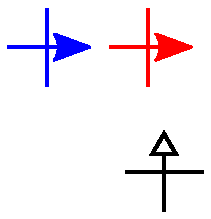
\includegraphics[width=\textwidth]{Figures/half_adder/schematic/000006_inputs_In1_0213/Input 0 deg.pdf}
    \caption{Input at \SI{0}{\degree}}
\end{subfigure}
\rulesep
\begin{subfigure}[t]{0.23\textwidth}
    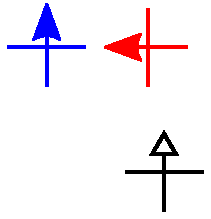
\includegraphics[width=\textwidth]{Figures/half_adder/schematic/000006_inputs_In1_0213/Input 90 deg.pdf}
    \caption{Input at \SI{90}{\degree}}
\end{subfigure}
\rulesep
\begin{subfigure}[t]{0.23\textwidth}
    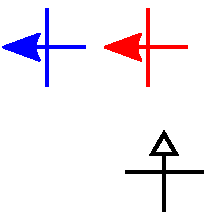
\includegraphics[width=\textwidth]{Figures/half_adder/schematic/000006_inputs_In1_0213/Input 180 deg.pdf}
    \caption{Input at \SI{180}{\degree}}
\end{subfigure}
\rulesep
\begin{subfigure}[t]{0.23\textwidth}
    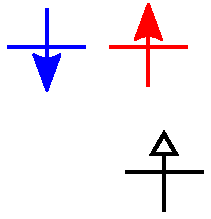
\includegraphics[width=\textwidth]{Figures/half_adder/schematic/000006_inputs_In1_0213/Input 270 deg.pdf}
    \caption{Input at \SI{270}{\degree}}
\end{subfigure}
\caption{Lowest energy configurations for all four possible input magnetizations. This functions as a half adder with quaternary convention $(0,2,1,3)$. Islands with a filled arrowhead (here the two at the top) can move their magnetization freely to achieve the lowest energy. Islands with an open arrowhead (here the one at the bottom) have their magnetization fixed in the direction of the arrow. The blue island in the top left corner is the input island, the red island in the top right corner functions as the output.}
\label{fig:HalfAdder_000006_configurations_In1_0213}
\end{figure}

In order to gain a more intuitive understanding of the states of a half adder and what they mean for the magnetization direction, in order to come up with a simple geometry that can be interpreted as a half adder, it is instructive to reformulate the half adder truth table~\ref{tab:HalfAdder} into three basic rules:
\begin{enumerate}
    \item There must be exactly two inputs for which input and output are equal. In the truth table this is $0\rightarrow0$ and $1\rightarrow1$.
    \item Exactly two inputs must both yield the same output. For one of these, the input must also be equal to the output, as in rule 1. In the truth table this is $1\rightarrow1$ and $2\rightarrow1$.
    \item For the final remaining input which does not fall under the previous rules, the output must be that input from the second rule which is not the same as its output. In the truth table this is $3\rightarrow2$.
\end{enumerate}
The first and second rules are quite straightforward, and form the basis for the reasoning behind the simplest biaxial half adder which will be discussed in this section. The third rule is quite complicated, and is thus not easily used when one tries to design a half adder geometry. It should rather be used to confirm the functioning of a half adder geometry once such a geometry seems promising. \par
From the discussion in \cref{par:TwoIslands_InteractionAngle} about the interaction between two islands, we know that two islands aligned along their hard axes preferably orient their magnetizations in the same direction along their common axis (as in \cref{fig:two-islands_interaction_(r0.66_L100)_a0and0}). This property can be exploited to fulfill the first rule of a half adder, i.e. there must be exactly two inputs for which the output and input lay in the same direction. So, two axis-aligned free islands form the basis of the half adder geometry. In the following, we will always place these two islands with their centres \SI{128}{\nano\metre} apart, such that there is \SI{28}{\nano\metre} of free space between them. One of these two islands will be considered the input, the other the output. The first rule has already shown that it is instructive to define \SI{0}{\degree} as 0 and \SI{180}{\degree} as 1, or vice versa. For the other two possible inputs, namely those perpendicular to the islands' common axis, the output preferably orients itself in the opposite direction as the input, such that indeed there are exactly only two inputs for which output and input lay in the same direction. Thus, the first rule of the half adder is fulfilled. \par
What is left to do now, is to break the symmetry to fulfill the second and third rules, by placing a fixed island near the two free islands. Practically, a fixed island can be manufactured by making use of the exchange bias as described in \cref{par:Intro_nanomagnetic-islands}. What we want, is that for one of the remaining inputs, which are perpendicular to the two islands' common axis, the output is parallel to this common axis, to fulfill rule 2 which states that exactly two situations must have the same output direction. This can be achieved by placing the fixed island away from the free islands' common axis, facing towards the output island, as shown schematically in \cref{fig:HalfAdder_000006_configurations_In1_0213}. This prevents the output island from having its magnetization pointing down, and will hence preferably point horizontally. To make the magnetization consistently choose either left or right, the fixed island is placed slightly away from the output's vertical axis. For example, in the figure the fixed island was placed slightly off to the right, such that the output slightly prefers a left magnetization over a right magnetization. \par
The third rule states that the output for the final remaining input must not be in the same direction as its input, and must also not be in any of the previous output directions, so not horizontal. As such, in this case it is allowed and even useful for this to be perpendicular to the islands' common axis, because the magnetizations will align anti-parallel. The fixed island does not impede this whatsoever, on the contrary, the output is even encouraged into this correct orientation, such that also this third rule is easily satisfied. The lowest energy configuration for each of the 4 possible inputs is shown in the schematic representation of \cref{fig:HalfAdder_000006_configurations_In1_0213}.

\begin{figure}
    \centering
    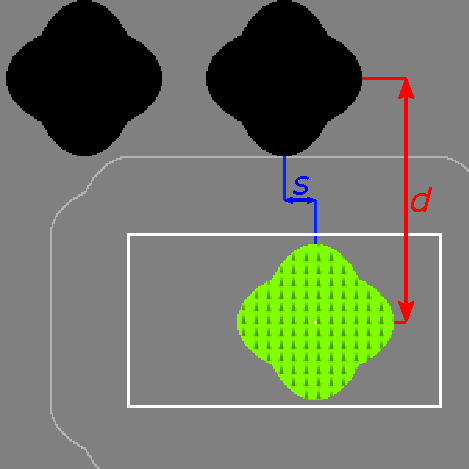
\includegraphics[width=0.35\textwidth]{Figures/half_adder/regions000006.pdf}
    \caption{Typical geometry of the half adder under discussion, with $(\rho, L) = (0.66, \SI{100}{\nano\metre})$ islands. The magnetization of the green island is permanently fixed at \SI{90}{\degree}. The black islands are free. The white rectangle indicates the range of the center of the green island, as examined in \cref{fig:HalfAdder_000006_sweep_d-s_balanced1}~and~\ref{fig:HalfAdder_000006_sweep_d-s_balanced2}. The thin grey line shows the farthest outline of the fixed island when moving its center throughout the white rectangle. The definition of $s$ and $d$ is also given.}
    \label{fig:HalfAdder_000006_geometryTypical}
\end{figure}

\begin{figure}
\centering
\begin{subfigure}[t]{0.37\textwidth}
    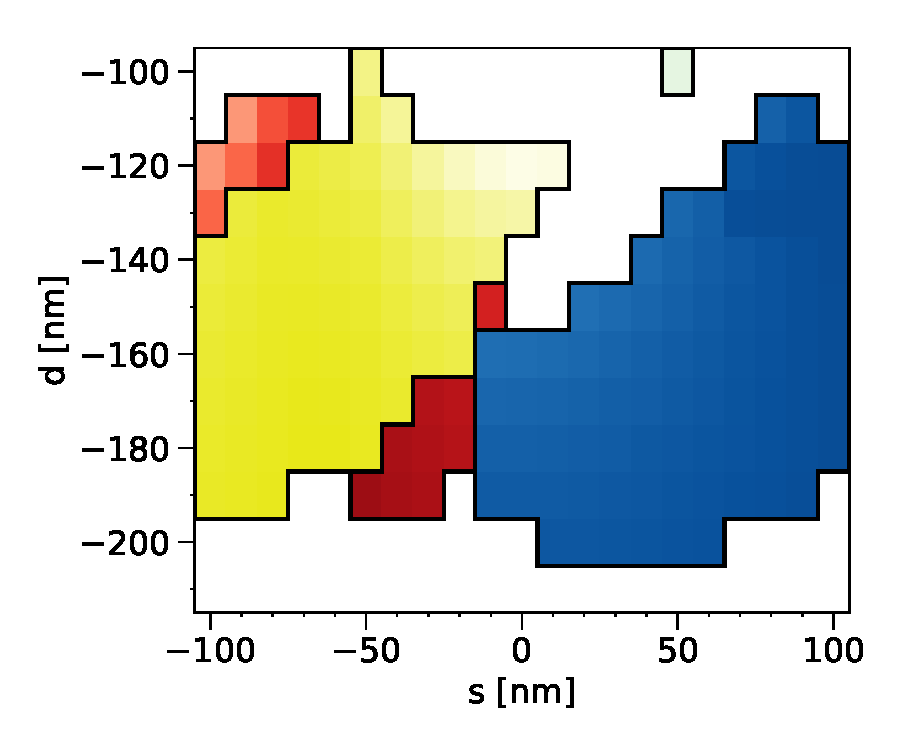
\includegraphics[width=\textwidth]{Figures/half_adder/sweep/000006_d-s/table(d100-210_10,s-100-100_10)_balanced1_reversedForeground.pdf}
\end{subfigure}
\begin{subfigure}[t]{0.62\textwidth}
    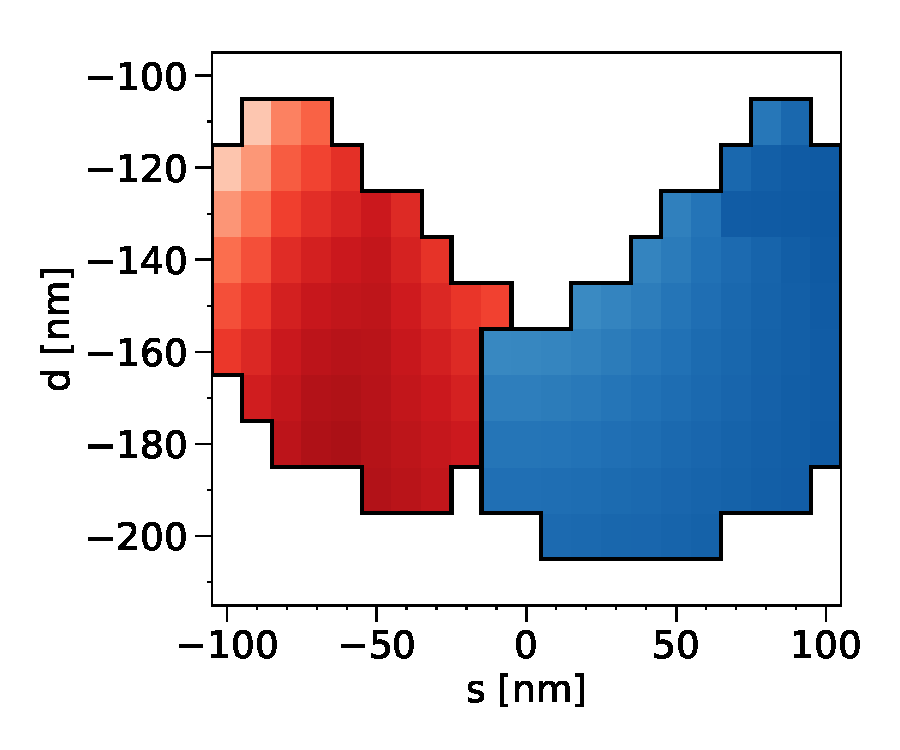
\includegraphics[width=\textwidth]{Figures/half_adder/sweep/000006_d-s/table(d100-210_10,s-100-100_10)_balanced1.pdf}
\end{subfigure}
\caption{Regions where the geometry, with the fixed island at position $(s, d)$ with respect to the output island, functions as a half adder according to the quaternary conventions indicated by the color. $M_{sat} = \SI{800}{\kilo\ampere\per\metre}$ for all islands. The darkness represents the first balancedness metric $B_1 = \min_\alpha(E_{\alpha,1}) - \max_\alpha(E_{\alpha,0})$. Because the red and yellow quaternary conventions overlap, the figure is shown twice, once with each color on the foreground.}
\label{fig:HalfAdder_000006_sweep_d-s_balanced1}
\end{figure}

\begin{figure}
\centering
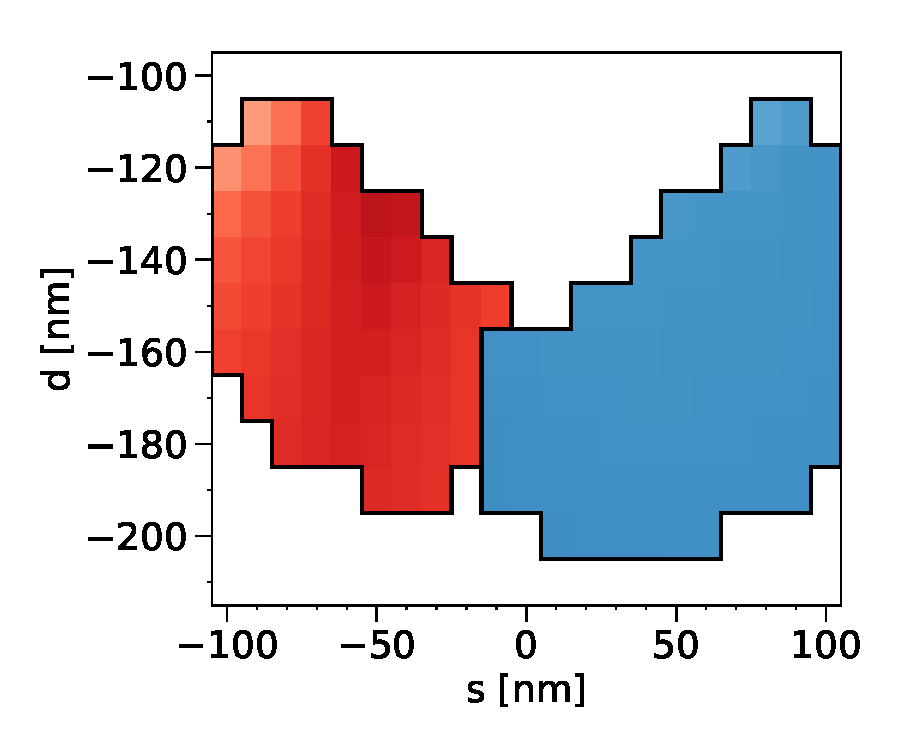
\includegraphics[width=0.9\textwidth]{Figures/half_adder/sweep/000006_d-s/table(d100-210_10,s-100-100_10)_balanced2.pdf}
\caption{Regions where the geometry, with the fixed island at position $(s, d)$ with respect to the output island, functions as a half adder according to the quaternary conventions indicated by the color. $M_{sat} = \SI{800}{\kilo\ampere\per\metre}$ for all islands. The darkness represents the second balancedness metric $B_2 = \max_\alpha(E_{\alpha,0}) - \min_\alpha(E_{\alpha,0})$.} 
\label{fig:HalfAdder_000006_sweep_d-s_balanced2}
\end{figure}





The typical geometry of this kind of half adder is shown in \cref{fig:HalfAdder_000006_geometryTypical}. The definition of the parameters $s$ and $d$ is also given in this figure: $s$ is the horizontal displacement of the fixed island, while $d$ is the difference in vertical position between the center of the fixed island and the center of the leftmost free island. The sign of $s$ and $d$ is defined in the usual mathematical manner, e.g. both $s$ and $d$ are negative when the island is to the lower left of the leftmost free island. \par 
The position $(s,d)$ of the fixed island will now be varied, as well as its saturation magnetization $M_{sat}$, to determine regions where the geometry correctly functions as a half adder, and to eventually find a position where the geometry is as balanced as possible. First, $s$ and $d$ will be varied in the region below the free islands, holding true to the initial reasoning presented earlier, which will reveal some symmetries. Later on, a similar treatment of the region near the common axis of the free islands will be given, which will yield more balanced half adders capable of reverse calculation, but with smaller error margins.

\subsubsection{Fixed island away from the common axis}
The results of varying $s$ from \SIrange{-100}{100}{\nano\metre} and $d$ from \SIrange{-100}{-210}{\nano\metre} are shown in figures~\ref{fig:HalfAdder_000006_sweep_d-s_balanced1}~and~\ref{fig:HalfAdder_000006_sweep_d-s_balanced2}. We will first explain the different colors in these figures, and only later discuss the brightness of these colors. The colored regions in these figures, surrounded by black contours, are the regions where the position of the fixed island is as such, that the geometry correctly functions as a half adder. The different colors, viz. blue, red, yellow and green, indicate what the correct quaternary convention is for that specific set of $s$ and $d$, as well as which of the two free islands is chosen a the input island; `In L' indicates that the leftmost free island is considered the input island, `In R' for the other island. There exists a region where both the red and yellow conventions are correct, so in \cref{fig:HalfAdder_000006_sweep_d-s_balanced2} the same figure is shown twice, once with each of these two colors on the foreground. \par
The blue region corresponds to the quaternary convention and choice of input island as it was conceived initially, which was shown schematically in \cref{fig:HalfAdder_000006_configurations_In1_0213}. \par
A first observation can be made by comparing the conventions of the red and blue regions. They both define the leftmost island as the input, and their quaternary conventions are nearly equal, the only difference being that their definition of $0$ and $1$ is opposite. This is easily understood, as the definition of 1 is determined by which of the two horizontal directions is preferred by the output island when the input is 2, which for both conventions is at \SI{90}{\degree}. This depends on the horizontal position of the fixed island. If the fixed island is placed more to the left, the magnetization of the free island will be more inclined to point to the right. This explains why the red and blue regions are nearly identical, and separated near the $s=0$ line. \par
The blue region does, however, extend a bit to the left of the $s=0$ line. This is because the fixed island is to the bottom right of the leftmost free island, such that the magnetization of the leftmost island has a slight tendency to point to the left, due to the dipolar field interaction with the fixed island. As such, if the fixed island is placed directly underneath the rightmost free island, this rightmost island will still have a preference for its magnetization to point to the left. This explains why the blue region extends to negative $s$-values, before transitioning to the red region. If the leftmost free island would not exist, and the fixed island would be placed directly below the leftmost free island, the free island would not have a preference for its magnetization to point left or right. \par
The limits of $d$ for the red and blue regions are also easily understood. For $d>\SI{200}{\nano\metre}$, the fixed island is too far away for the geometry to function as a half adder. The entire functioning of the half adder, as it was initially conceived, rests on the fixed island preventing the leftmost island from having an average magnetization angle near \SI{270}{\degree}, but rather horizontal at \SI{0}{\degree} or \SI{180}{\degree}. As it turns out, for $(\rho, L) = (0.66,\SI{100}{\nano\metre})$ islands with a saturation magnetization $M_{sat}$ of \SI{800}{\kilo\ampere\per\metre}, the center of the fixed island should not lay further than \SI{200}{\nano\metre} away from the common axis of the two free islands. Conversely, there also exists a lower limit: the fixed island must not lay too close to the free islands, because then even a horizontal magnetization becomes unfavorable for them. \par
When comparing the yellow and red regions, a symmetry can be observed. In the yellow region, the rightmost island is considered the input island, which is opposite to the definition in the red region. Taking a look at their quaternary conventions, it is clear that they are each other's horizontally mirrored counterpart: the definitions of 0 and 1, corresponding to the horizontal directions \SI{0}{\degree} and \SI{180}{\degree}, are oppositely defined between the yellow and red conventions. This is because the entire geometry is symmetrical when the fixed island is placed at $s=\SI{-64}{\nano\metre}$, because the centres of the two free islands are spaced \SI{128}{\nano\metre} apart. The reason why \cref{fig:HalfAdder_000006_sweep_d-s_balanced2} is not perfectly symmetrical about the $s=\SI{-64}{\nano\metre}$ axis, is because this figure was calculated for a range of $s$ with steps of \SI{10}{\nano\metre}. It is easy to see that there will then also exist a mirrored counterpart for the blue region at even lower values for $s$. All these regions will also have a vertically mirrored counterpart for positive values of $d$. \par

We will now turn our attention to the brightness of the colors in the figures. Both in \cref{fig:HalfAdder_000006_sweep_d-s_balanced1} and \cref{fig:HalfAdder_000006_sweep_d-s_balanced2}, there is a greyscale colorbar, representing a different quantity for either figure. These quantities are different metrics to assess the balancedness of a half adder, based on the different energy levels of different input values. The first metric that can be used to assess the balancedness, is the energy difference between the highest ground state and the lowest first excited state, given by $B_1 = \min_\alpha(E_{\alpha,1}) - \max_\alpha(E_{\alpha,0})$. The meaning of $E_{\alpha,i}$ was already given: it is the $i$-th lowest energy level for which the input magnetization is at or near an angle $\alpha$. If one wants to use the half adder for a reverse calculation, $B_1$ should be positive. This would mean that the energies of all the correct ground states are lower than the energies $E_{\alpha,i}, i\neq 0$, of all the incorrect states. As such, when operating the half adder thermally, the correct states will have a higher probability of occurring than the incorrect ones, which allows to discriminate between correct and incorrect states in a purely statistical manner. \par
Ideally, for a perfectly balanced logic gate, the ground state energies for each of the 4 possible inputs of the input island should be equal. The degree to which this condition is fulfilled is represented by the second metric $B_2 = \max_\alpha(E_{\alpha,0}) - \min_\alpha(E_{\alpha,0})$: the energy difference between the highest and lowest of the 4 ground states. Evidently, this is always positive. If this is zero, the half adder is perfectly balanced. The higher $B_2$, the less balanced the half adder is.
Hence, in the greyscales of the figures, the most balanced half adders are the darkest, and the least balanced ones the brightest. When searching for a half adder suitable for reverse calculation, the most important metric at first is $B_1$. Once $B_1$ is positive, one can assess $B_2$, which should be minimal. \par
Figure~\ref{fig:HalfAdder_000006_sweep_d-s_balanced1} shows the first metric $B_1$. Unfortunately, the second metric is always negative in the examined range where the fixed island is placed away from the common axis of the free islands, such that none of these half adders can be used for a reverse calculation. The optimal values do come close to zero, though, especially near $s=\SI{-60}{\nano\metre}$ and $d=\SI{-170}{\nano\metre}$. The energy levels corresponding to the half adder at these coordinates are explicitly shown in \cref{fig:HalfAdder_000006_energylevels_d170_s-60}.
\begin{figure}
    \centering
    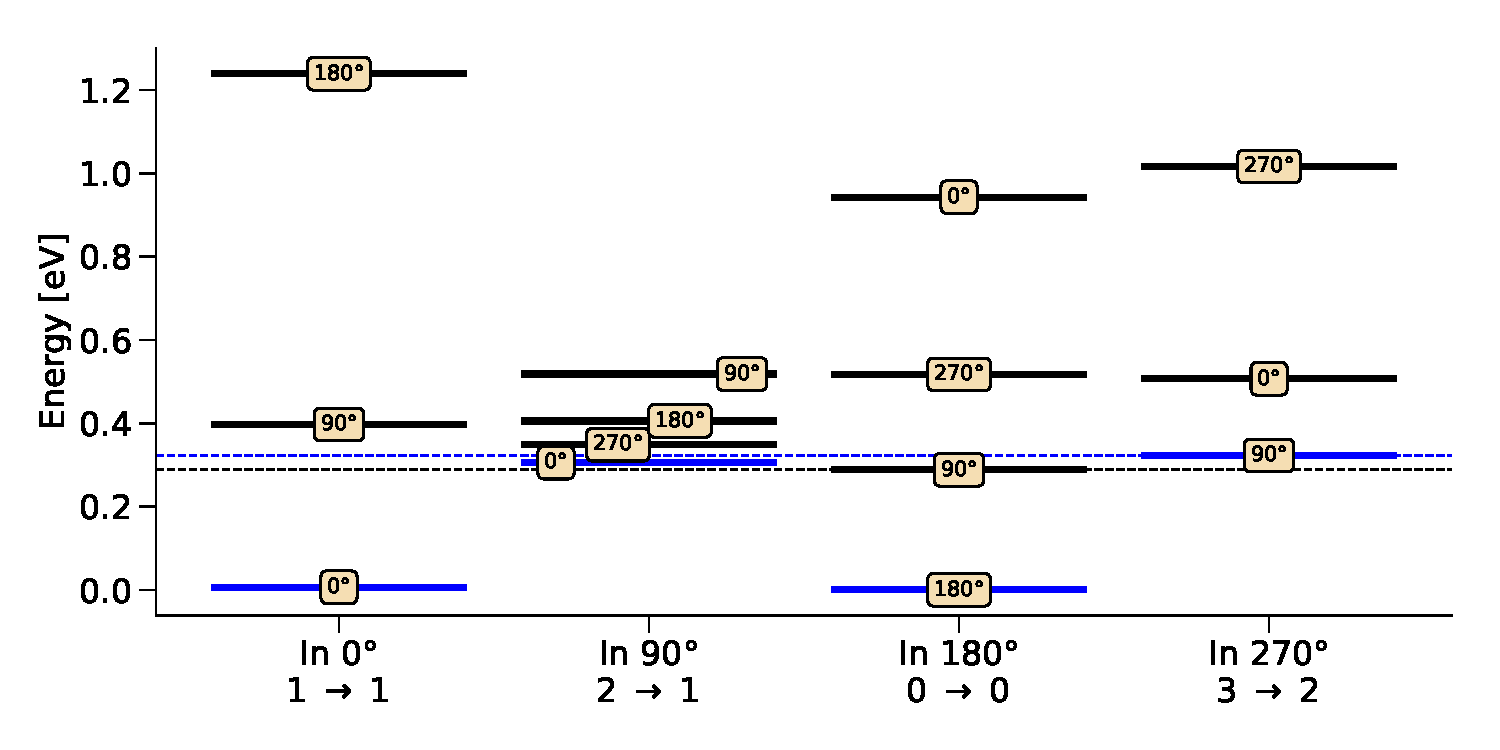
\includegraphics[width=0.9\textwidth]{Figures/half_adder/energylevels/table(d170,s-60)_energylevels.pdf}
    \caption{Energies of different magnetization configurations, grouped by input magnetization angle, for a half adder with $d=\SI{-170}{\nano\metre}$ and $s=\SI{-60}{\nano\metre}$, and $M_{sat} = \SI{800}{\kilo\ampere\per\metre}$ for all islands. The orientation of the output island is shown in the text box for each energy level. The lowest energy level for each input is indicated in blue. The quaternary convention, dictated by these energy levels, is given at the bottom: the number before the arrow gives the input for that column, the number after the arrow the output for the lowest energy level of that column.}
    \label{fig:HalfAdder_000006_energylevels_d170_s-60}
\end{figure}
In this figure, the energy levels are grouped by input. The angle in the text box of each energy level represents the output magnetization responsible for that energy level. This figure can make the meaning of balancedness a bit clearer. The highest ground state in this case is for a \SI{270}{\degree} input, while the lowest first excited state $E_{\SI{180}{\degree}, 1}$ is the one for a \SI{180}{\degree} input with \SI{90}{\degree} output. This incorrect output clearly has a lower energy than the correct output for the \SI{270}{\degree} input, as clarified by the dotted lines extending horizontally. \par
Some other observations can also be made from these energy levels. Firstly, the energy levels for the input at \SI{90}{\degree} are much more closely spaced than for other inputs. This is because the entire functioning of the half adder rests on the fixed island preventing this input from having its output pointing down. This means the geometry can not relax as it normally would, such that the energies are all pushed together. If the fixed island would be placed even further, the \SI{270}{\degree} level would fall below the \SI{0}{\degree} level, and the geometry would no longer function as a half adder. This was already remarked from the extent of the red and blue regions in \cref{fig:HalfAdder_000006_sweep_d-s_balanced1}.
Secondly, $E_{\SI{0}{\degree}, 2}$ corresponding to an output at \SI{180}{\degree}, has a higher energy than $E_{\SI{180}{\degree}, 3}$ corresponding to an output at \SI{0}{\degree}. This is for the same reason which has been brought up a few times already; the island prefers a magnetization away from the fixed island, and for this half adder the fixed island is to the bottom left of the output island.
Finally, it can be remarked that there are some inputs which have less than four energy levels. This is because the combination of magnetization angles corresponding to the absent energy levels is not stable. During the relaxation, the magnetization of an island can rotate over more than \SI{90}{\degree} to reach an energy minimum. As such, multiple initial configurations can reach the same energy minimum, reducing the total number of energy levels in the figure. \par

We now return to \cref{fig:HalfAdder_000006_sweep_d-s_balanced2}, which shows the second metric $B_2$ in its greyscale. Since the first metric is negative everywhere in the $(s,d)$-region of the figure, the half adders can not be used for reverse calculation. Forward calculation is still possible for any of the colored regions, and the second metric shows how well-suited a certain choice of $s$ and $d$ is for this purpose. The best values are clearly near $s=\SI{-50}{\nano\metre}$ and $d=\SI{-130}{\nano\metre}$, so it is best to use those values for a forward-calculating half adder of this type. The blue region does not show a lot of variation and has a rather high value of $B_2$ everywhere, and can thus be disregarded for forward calculation.

In the figures, there is also the green half adder with quaternary convention $(1,3,0,2)$, which is the small region at $(s,d) = (50, -100) \si{\nano\metre}$. It is clearly not suited at all as it scores bad for both $B_1$ and $B_2$. The region is also very small, which could make it difficult to reliably manufacture the corresponding geometry. Therefore, this region was not investigated further.


\begin{figure}
    \centering
    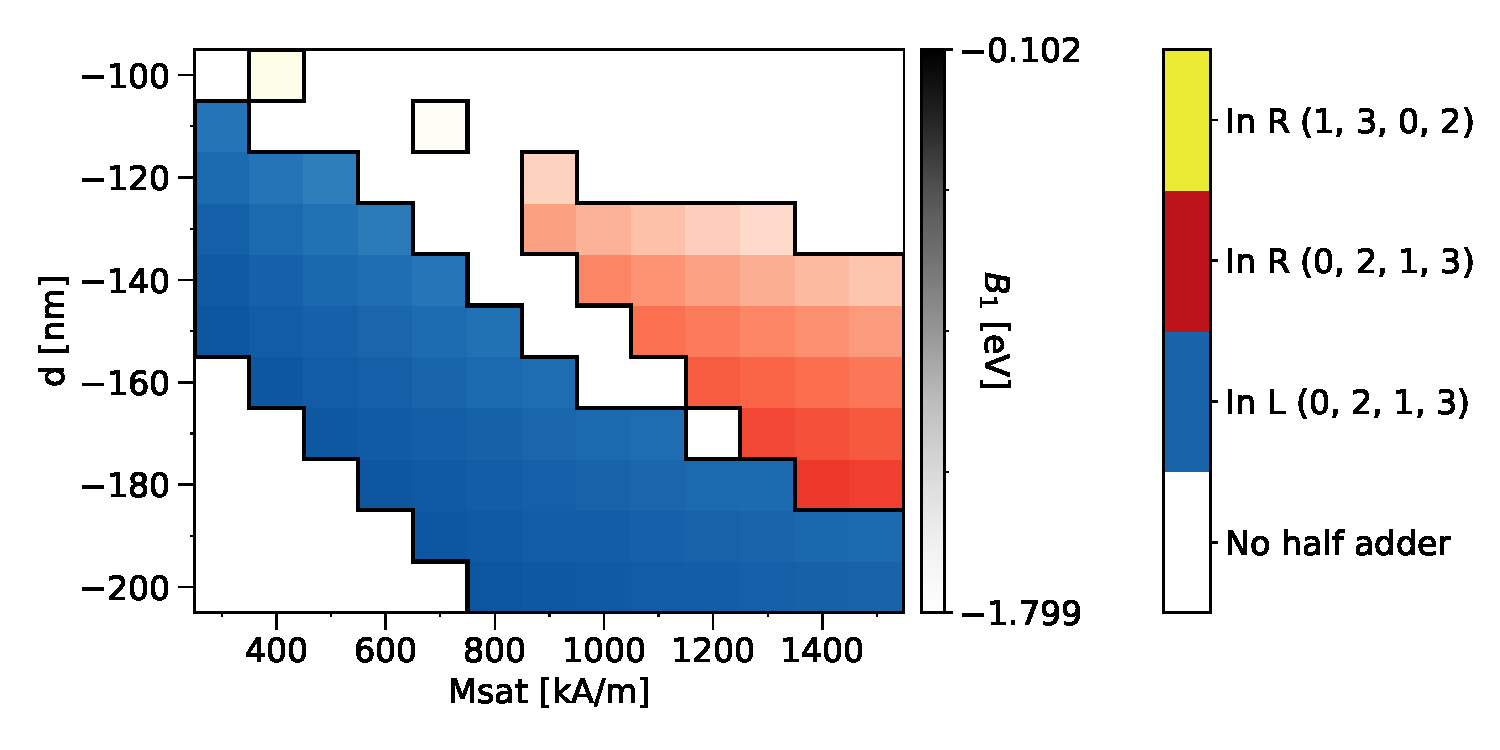
\includegraphics[width=0.9\textwidth]{Figures/half_adder/sweep/000006_d-Msat/table(d100-200_10,Msat3e5-15e5_1e5)_balanced1.pdf}
    \caption{Regions where the geometry, with the fixed island at position $(s=\SI{20}{\nano\metre}, d)$ with respect to the output island, functions as a half adder according to the quaternary conventions indicated by the color. The saturation magnetization of the fixed island is changed, while for the free islands it remains at $M_{sat} = \SI{800}{\kilo\ampere\per\metre}$. The darkness represents the first balancedness metric: $B_1 = \min_\alpha(E_{\alpha,1}) - \max_\alpha(E_{\alpha,0})$.} 
    \label{fig:HalfAdder_000006_sweep_d-Msat_balanced1}
\end{figure}
Another parameter sweep was also conducted, as shown in \cref{fig:HalfAdder_000006_sweep_d-Msat_balanced1}, where the saturation magnetization $M_{sat}$ and the vertical position $d$ were varied. What is immediately clear from this figure is that the region with functioning half adders is quite linear: the further away the fixed island is, the larger its saturation magnetization must be to remain influential enough for the gate to behave as a half adder. The role of the left and right islands also seems to switch at a certain point, as evidenced from the red region taking over at smaller $d$, which can be explained by the fact that, the further away the fixed island is, the more equal the field will be for both of the free islands. \par
The sweeping of $M_{sat}$ shows that placing the fixed island further away makes the logic gate more balanced. This is logical, as increasing this distance decreases the interaction between the fixed island and the free islands. In the absence of the fixed island, the two free islands have a lot of symmetry, such that there are some magnetization configurations with equal energy. Including the fixed island breaks this symmetry and moves these energy levels. Thus, the smaller the interaction with this fixed island, the closer these energies will remain to each other, and the more balanced the logic gate will remain. \par


In conclusion, the standard reasoning behind this type of geometry, as explained some paragraphs ago, clearly does not work. The question is now, whether there exists a combination of $s$ and $d$ for which $B_1$ is positive. For this, a different range of $s$ and $d$ was examined, which places the fixed island near the common axis of the free islands. This is the subject of the next section.


\subsubsection{Fixed island near the common axis}
\begin{figure}
    \centering
    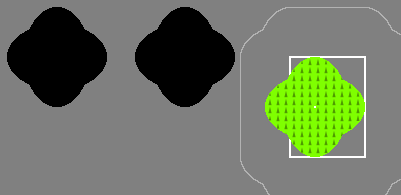
\includegraphics[width=0.35\textwidth]{Figures/half_adder/regions000014.png} % TODO: larger or not? depends on if it fits on previous page
    \caption{Typical geometry of the half adder with the fixed island near the common axis, with $(\rho, L) = (0.66, \SI{100}{\nano\metre})$ islands. The magnetization of the green island is permanently fixed at \SI{90}{\degree}. The black islands are free. The white rectangle indicates the range of the center of the fixed island, as examined in \cref{fig:HalfAdder_000006_sweepnew_d-s_balanced1}~and~\ref{fig:HalfAdder_000006_sweepnew_d-s_balanced2}. The thin grey line shows the farthest outline of the fixed island when moving its center throughout the white rectangle.}
    \label{fig:HalfAdder_000006new_geometryTypical}
\end{figure}
\begin{figure}
    \centering
    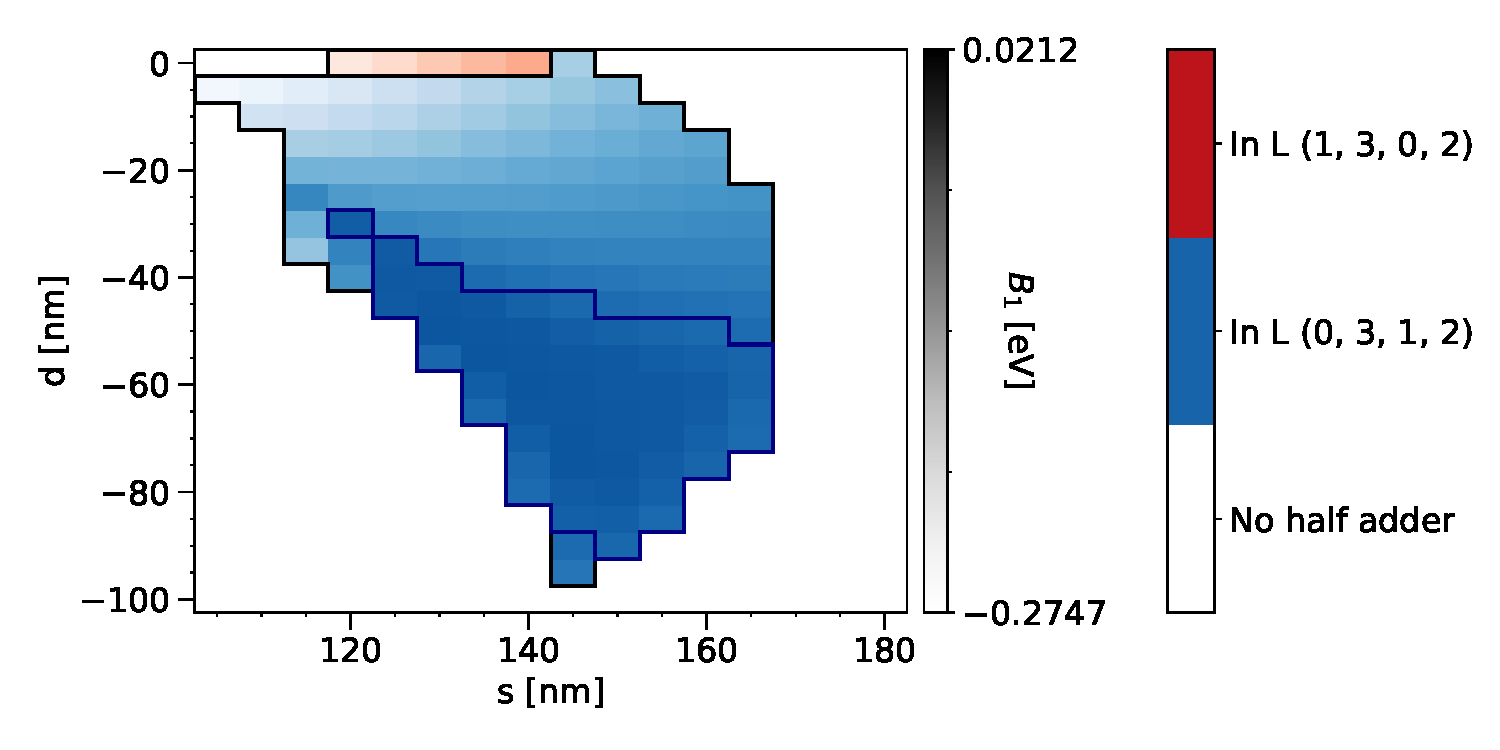
\includegraphics[width=0.9\textwidth]{Figures/half_adder/sweep/000006_d-s/tableside(d0-100_5,s100-180_5)_balanced1.pdf}
    \caption{Regions where the geometry, with the fixed island at position $(s, d)$ with respect to the output island, functions as a half adder according to the quaternary conventions indicated by the color. The darkness represents the first balancedness metric: $B_1 = \min_\alpha(E_{\alpha,1}) - \max_\alpha(E_{\alpha,0})$. Inside the dark blue outline, $B_1$ is positive.} 
    \label{fig:HalfAdder_000006_sweepnew_d-s_balanced1}
\end{figure} % TODO: is this outline color good or better yellow (quite obnoxious) or grey (also quite bright idk)
\begin{figure}
    \centering
    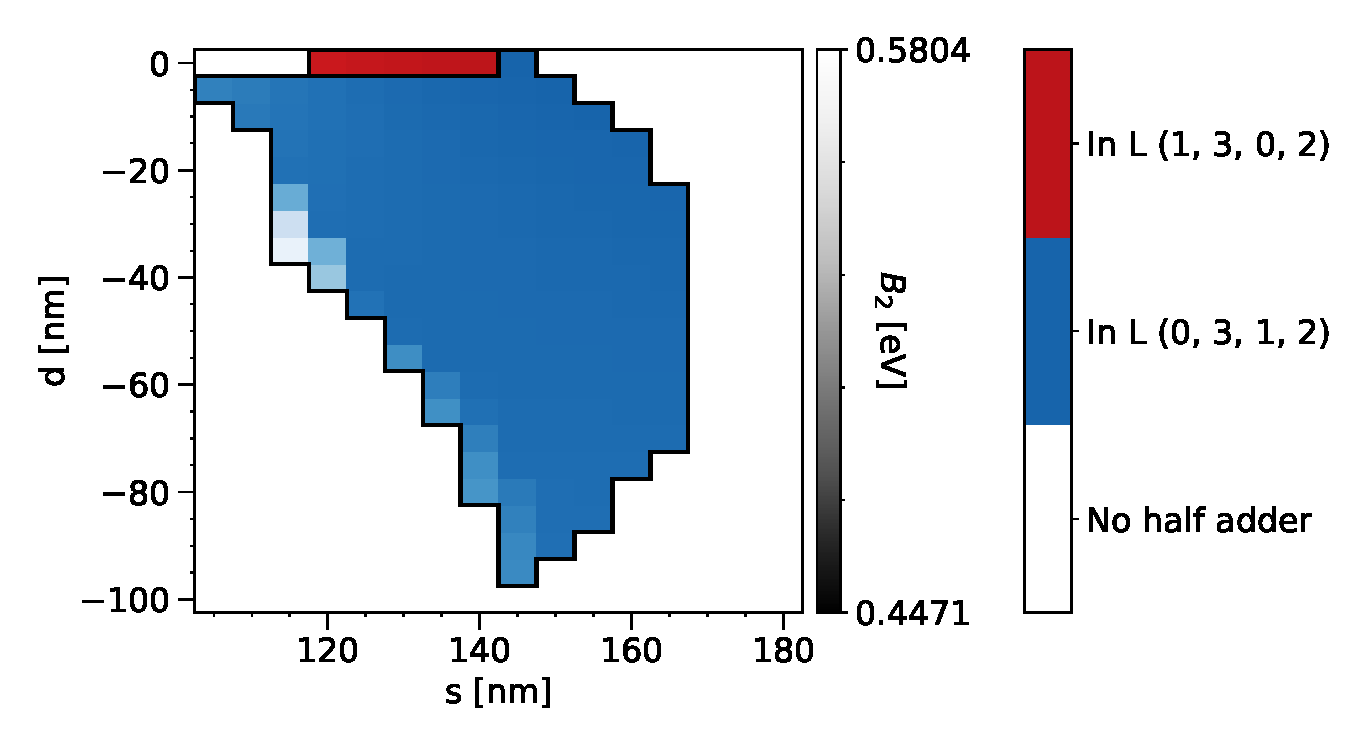
\includegraphics[width=0.9\textwidth]{Figures/half_adder/sweep/000006_d-s/tableside(d0-100_5,s100-180_5)_balanced2.pdf}
    \caption{Regions where the geometry, with the fixed island at position $(s, d)$ with respect to the output island, functions as a half adder according to the quaternary conventions indicated by the color. The darkness represents the first balancedness metric: $B_2 = \max_\alpha(E_{\alpha,0}) - \min_\alpha(E_{\alpha,0})$.} 
    \label{fig:HalfAdder_000006_sweepnew_d-s_balanced2}
\end{figure}
\begin{figure}
    \centering
    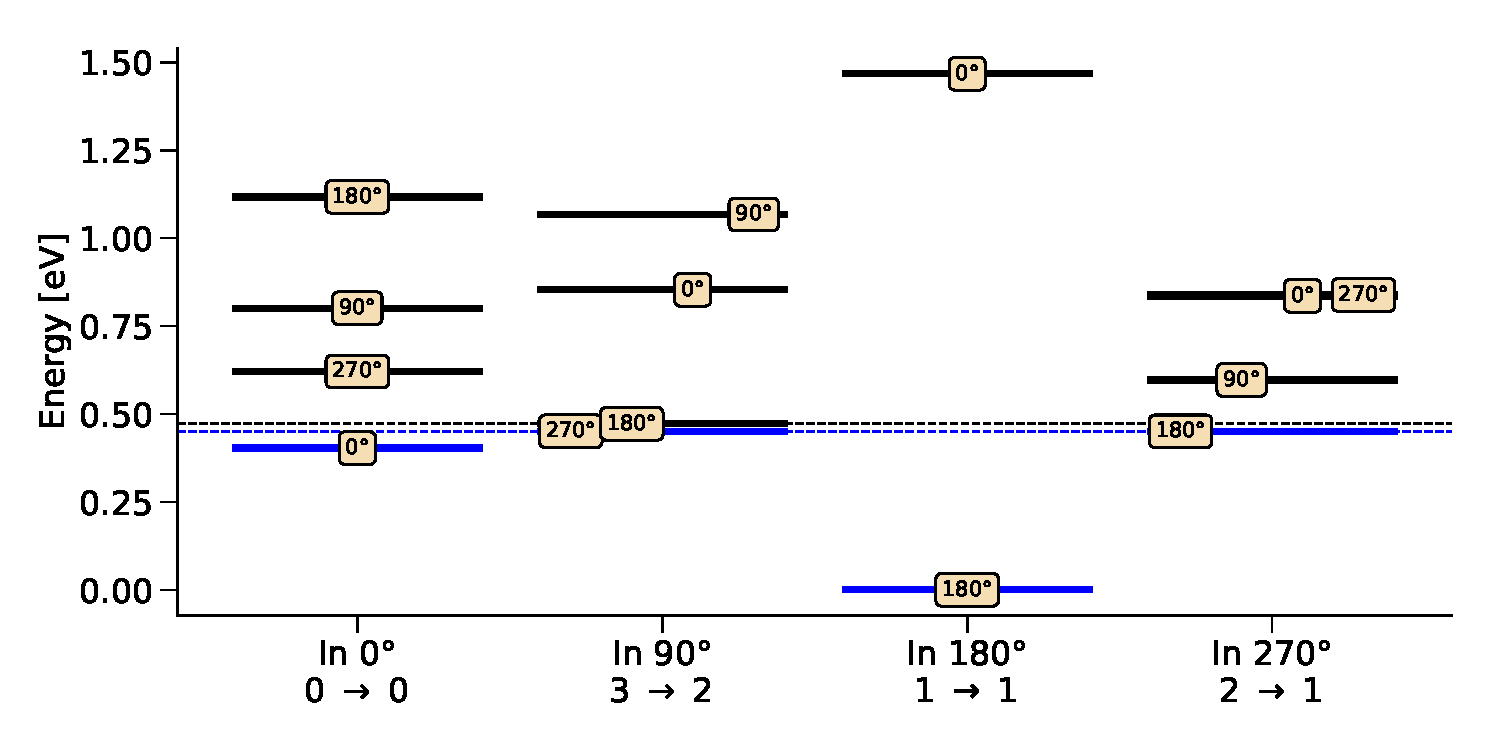
\includegraphics[width=0.9\textwidth]{Figures/half_adder/energylevels/tableside(d50,s130)_energylevels.pdf}
    \caption{Energies of different magnetization configurations, grouped by input magnetization angle, for a half adder with $d=\SI{-50}{\nano\metre}$ and $s=\SI{130}{\nano\metre}$, and $M_{sat} = \SI{800}{\kilo\ampere\per\metre}$ for all islands. The orientation of the output island is shown in the text box for each energy level. The lowest energy level for each input is indicated in blue. The quaternary convention, dictated by these energy levels, is given at the bottom: the number before the arrow gives the input for that column, the number after the arrow the output for the lowest energy level of that column.}
    \label{fig:HalfAdder_000006_energylevels_d50_s130}
\end{figure}
\begin{figure}
    \centering
    \begin{subfigure}[t]{0.23\textwidth}
        \includegraphics[width=\textwidth]{Figures/half_adder/schematic/000006side_inputs_In1_0312/Input 0 deg.pdf}
        \caption{Input at \SI{0}{\degree}}
    \end{subfigure}
    \rulesep
    \begin{subfigure}[t]{0.23\textwidth}
        \includegraphics[width=\textwidth]{Figures/half_adder/schematic/000006side_inputs_In1_0312/Input 90 deg.pdf}
        \caption{Input at \SI{90}{\degree}}
    \end{subfigure}
    \rulesep
    \begin{subfigure}[t]{0.23\textwidth}
        \includegraphics[width=\textwidth]{Figures/half_adder/schematic/000006side_inputs_In1_0312/Input 180 deg.pdf}
        \caption{Input at \SI{180}{\degree}}
    \end{subfigure}
    \rulesep
    \begin{subfigure}[t]{0.23\textwidth}
        \includegraphics[width=\textwidth]{Figures/half_adder/schematic/000006side_inputs_In1_0312/Input 270 deg.pdf}
        \caption{Input at \SI{270}{\degree}}
    \end{subfigure}
    \caption{Lowest energy configurations for all four possible input magnetizations. This functions as a half adder with quaternary convention $(0,3,1,2)$. Islands with a filled arrowhead are free, islands with an open arrowhead are fixed. The blue island at the left is the input island, the red island in the middle the output.}
\label{fig:HalfAdder_000006side_configurations_In1_0312}
\end{figure}

A different region where the fixed island can allow the geometry to function as a half adder is shown in \cref{fig:HalfAdder_000006_sweepnew_d-s_balanced1}. In this figure, $s$ was varied from \SI{110}{\nano\metre} to \SI{180}{\nano\metre}, and $d$ from \SI{0}{\nano\metre} to \SI{100}{\nano\metre}. This region is also illustrated on the geometry of \cref{fig:HalfAdder_000006new_geometryTypical}, as the white rectangle. Note that the colors of these regions have no connection whatsoever to the colors of the regions from the previous paragraph; the quaternary conventions observed here have not been encountered before. \par
For $d=\SI{0}{\nano\metre}$, the geometry is perfectly symmetric, such that the horizontally mirrored counterpart of the blue region, i.e. the red region, shows up at $d \geq 0$. The red region is simply the mirrored counterpart of the blue region about the $d=0$ line. At first sight, one might wonder why these two regions are equivalent, as the magnetization direction of the fixed island is `up' for both, so they are not each other's mirror image. They are equivalent, however, if one is only interested in the energy levels, because the energy levels are invariant under a global magnetization reversal. As the fixed island is magnetized vertically, this explains the vertical symmetry in space. Furthermore, the quaternary convention of the red region is identical to that of the blue region, but flipped horizontally. This is because a magnetization reversal is equivalent to one vertical and one horizontal mirroring, and additionally the red and blue regions are each other's vertical mirror image in space. The vertical mirroring occurs twice, which cancels itself, leaving only the horizontal mirroring which is observed in the quaternary convention. \par
The quaternary convention $(0,3,1,2)$ encountered here is simply the vertically mirrored counterpart of the previous blue region from \cref{fig:HalfAdder_000006_sweep_d-s_balanced1} which had $(0,2,1,3)$. This can be understood from the dipolar field of the fixed island. Previously, this dipolar field was mainly pointing up near the free islands, because the fixed island was placed below them. Now, the fixed island is more to the side, so because the dipolar field curls back on itself, the field near the free islands is now pointing down. Hence, the quaternary convention is also flipped vertically. \par
In contrast to the half adders from the previous section, there are now some values of $(s,d)$ for which the first balancedness metric $B_1 = \min_\alpha(E_{\alpha,1}) - \max_\alpha(E_{\alpha,0})$ is positive! This means that the gate can be used for at least one reverse calculation. The region in the $(s,d)$-plane where the metric is positive is also quite large, leaving a decent manufacturing error margin. One must note, however, that the maximal value for $B_1$ here is only \SI{21.2}{\milli\electronvolt}, which is lower than the room temperature $k_B T = \SI{25.8}{\milli\electronvolt}$, so the energy difference is still very small. \par
The second balancedness metric is shown in \cref{fig:HalfAdder_000006_sweepnew_d-s_balanced2}. Unfortunately, the minimal value of this second metric is \SI{0.447}{\electronvolt} throughout this region. For the regions in the previous section, with the fixed island far away from the common axis, this second metric could be as low as \SI{0.205}{\electronvolt}. The second metric is very constant throughout the blue region, and only increases close to the border at the bottom left of this region, so as long as the fixed island is not close to this border the second metric has no major influence. \par
The optimal value of these two metrics is thus located near $(s,d)=(\SI{130}{\nano\metre}, \SI{-50}{\nano\metre})$. The energy levels for that choice of $s$ and $d$ are shown in \cref{fig:HalfAdder_000006_energylevels_d50_s130}. As the first balancedness metric is now positive, the highest ground state is below the lowest first excited state, as is evident from the figure. The margin is quite small, however, which is not ideal. Because the fixed island is located to the bottom right of the free islands, all energy levels for an output at \SI{0}{\degree} are shifted up, while those for \SI{180}{\degree} are shifted down. The shift of energy levels is greatest for an input at \SI{180}{\degree}, there is not even a stable energy minimum for the output near \SI{90}{\degree} or \SI{270}{\degree}. Additional stabilization when the input at \SI{180}{\degree} could be useful in decreasing the energy difference between the ground states. \par
By comparing the energy levels to those of the half adder from the previous section, where the fixed island was placed far away from the common axis, one may notice that $\min_\alpha(E_{\alpha,1}-E_{\alpha,0})$ is quite a bit smaller in \cref{fig:HalfAdder_000006_energylevels_d50_s130}. This is the minimal energy difference between a ground state and its respective first excited state, and is a measure for how well suited the geometry is for forward calculation. Hence, the half adder from this section is worse at forward calculation than the one from the previous section, but it is capable of 1 reverse calculation while the one from the previous section is not. \par % TODO: maybe find a good name for 'the one from the previous section'
For the previous half adders with the fixed island far from the common axis, it was possible to add nanomagnetic chains to the input and output. Unfortunately, because the fixed island is now much closer to the common axis, adding a nanomagnetic chain to the output island has become nontrivial.

\subsubsection{Other geometries}
In the previous discussion, the position and saturation magnetization of the fixed island were varied to find their optimal values. Other parameters can also be adjusted, like the angle of this fixed island, or the angles of the free islands. Additional islands can also be added to create even more degrees of freedom. However, this geometry is fundamentally unbalanced, as the vertical direction is fundamentally different from the horizontal axis. \par
In order to find a half adder which is actually balanced, different geometries must be considered. Some more symmetrical geometries were examined in addition to the geometry discussed previously, but unfortunately no well-balanced half adder was found. The most promising shape with higher symmetry has four biaxial islands in a rhombus shape, with alternating \SI{45}{\degree} rotation, which contains a degenerate half adder if one takes a \SI{45}{\degree} rotated island as input and a non-rotated island as output. Somehow, one should include a fixed island into this geometry to unambiguously define the correct half adder convention, but no sufficiently symmetrical placement was found. \par
The only quaternary combinations found throughout the different geometries are all variations on $(0,2,1,3)$, reversed and/or cyclically permuted. No $(0,1,3,2)$ was found, which would be ideal for converting the biaxial information into uniaxial. This is because. \par %TODO
As is evident from the geometries that were previously discussed, having two islands in a `++' configuration does not impede the functioning of the half adder. Having more than two islands in line does, however, create a strong preference for the magnetization to align along that axis, which can cause the energy levels to shift significantly away from being balanced. Using the balanced `XX' chain does not prefer any of the four directions, and can thus be very useful to build a balanced half adder. The inherent inversion of the `XX' chain does not allow it to function as a half adder on its own, like the half adders discussed in the previous paragraphs. However, the `XX' chain is balanced, so it can definitely be used as a part of an as of yet unknown balanced half adder geometry. \par
Of course, these are just general remarks, and it is not excluded that a particular geometry could function as a half adder while negating these remarks.


\clearpage
\section{Conclusion}
In order to gain an understanding of the behavior of a single island, the energy landscape and thermal switching were examined. A first major remark was that relaxation is necessary for anisotropy to occur. If the island has a perfectly uniform magnetization pointing in-plane in a certain direction, the energy is equal for all these directions. As such, it was necessary to \code{relax()} the magnetization profile in order to gain useful information about the energy barrier. This in turn necessitated the use of a `virtual' external field to prevent the magnetization from relaxing all the way to an energy minimum. \par
It was found that the energy barrier between stable states significantly depends on the roundness of the biaxial island. As a function of the roundness, different axes take the role of easy axes. For large roundnesses, the easy axes are the longest dimensions of the geometry, i.e. horizontal and vertical. For small roundnesses, the geometry resembles a `plus'-shape, such that each arm of this shape has its own preferred direction. The combination of such vertical and horizontal directions is on average diagonal, with a domain wall in between, hence the average magnetization appears to be diagonal. For this reason, one must take care when using a biaxial island with low roundness, as the magnetization in the different lobes can differ significantly. In between these two regimes, there exists a roundness $r\approx0.49$ for which the energy barrier is very low, and the higher order terms of the anisotropy become dominant such that there are 8 stable states instead of 4. \par
A balanced biaxial chain was proposed, which can be used to transmit biaxial information between different logic gates. The easy axes in such a chain are aligned in an `XX' pattern, such that a rotation or mirror symmetry leaves the system invariant. As a single biaxial island can represent two bits of information, it can be useful to extract these two bits individually. This is for example needed to add two numbers together which consist of more than 1 bit each. A solution was proposed to read the two bits magnetically in the $(0,1,3,2)$ quaternary convention. For other quaternary conventions, it should be possible to read these components out electronically, but an elegant way of doing this magnetically has not yet been found. This can be the subject of future work: how to extract each bit out of the biaxial island, and additionally how such a biaxial chain can be optimized for signal propagation, while examining the behavior of the energy levels when introducing bends or \SI{90}{\degree} turns in the chain. \par
%- Future work: extract each bit out of the quaternary 'bit', is extremely easy when 0132 order (just place uniaxial islands going away from the diagonals, though unfortunately that chain must be along the uniaxial island's easy axes which does not allow the procedures from literature as described in the introduction) but other orders I dont see how to get that out of a biaxial island, for example for the 0213 discussed above it is easy to get out the second bit (place islands along the diagonal between 0 and 2 states) but first bit is not possible or at least not obvious, somehow you would need to detect whether the magnetization is horizontal in either direction, or vertical in either direction. One can leave out the 11 output because that thing is useless anyway. Also initializing a biaxial nanomagnet from uniaxial inputs can be an interesting problem to research. Extracting each bit is necessary if one wants to put multiple half adders in series, because to add two two-bit numbers for example one needs three half adders, the third of which takes the carry and sum of either other half adder as inputs, thus requiring a decomposition of the biaxial information. TODO: put this discussion in the correct place earlier in the thesis
The two half adders detailed in \cref{par:halfadder} can both function in a forward calculation. The best of these, i.e. with the fixed island near the free islands' common axis, has all ground state energies below any of the first excited states, which ensures a correct functioning for a single reverse calculation under ideal circumstances. Unfortunately, in order to chain multiple gates together for a larger reverse calculation, all the ground state energies must be equal, i.e. the gate must be perfectly balanced, which is not the case. \par
The other type of half adder, with the fixed island relatively far away from the common axis, can not function in reverse at all, as it has excited states with lower energies than some ground states. This type of half adder does, however, have more spacing in between its energy levels, such that it is better suited for forward calculation. It also has the advantage that it should be relatively straightforward to add some nanomagnetic chains to the input and output, as the fixed island is placed far away from their common axis. \par
Unfortunately, any half adder following the same concept of using two in-line biaxial islands will never have the ideal quaternary convention $(0,1,3,2)$, because a central part of the reasoning behind this concept requires 0 and 1 to have opposite direction. To resolve these various issues, a radically different geometry will have to be conceived. \par
The main subject of future work can be the continuation of a search for a balanced half adder. A completely new geometry should be designed which is inherently more symmetrical. The asymmetry in the quaternary truth table might prevent a truly mathematically balanced half adder. Including more islands can increase the degrees of freedom, such that a balanced half adder can be approximated by varying geometrical and material parameters.


\newpage
\bibliographystyle{bibliography/unsrtnat2}
\bibliography{bibliography/bibliography.bib}


\end{document}

% TODO AT THE END:
% - Have as few as possible 'radians' instead of 'degrees' This can be done by searching for \pi
